\documentclass[12pt,a4paper]{article}
\usepackage{graphicx}
\usepackage{minted}
\usepackage{float}
\usepackage{multicol}
\usepackage{multirow}
\usepackage[english,magyar]{babel}
%\usepackage{hyperref}
%\usepackage{comment}
\usepackage{ragged2e}
\usepackage{biblatex}
\usepackage{amsmath}
\usepackage{titling}


\newcommand{\firstpage}{
\thispagestyle{empty}
\vspace*{5mm}
\begin{center}
    {\Large Széchenyi István Egyetem\\}
    {\Large Gépészmérnöki, Informatikai és Villamosmérnöki Kar}
\end{center}
\vspace{35mm}
\begin{center}
    {\huge \bf DIPLOAMUNKA}
\end{center}
\vspace{35mm}
\begin{center}
    {\huge Péter Bence Gábor}
\end{center}
\vspace{3mm}
\begin{center}
   {\LARGE Mérnökinformatika BSc}
\end{center}
\vspace{35mm}
\begin{center}
   {\LARGE 2023}
\end{center}
{\small A gerincen:}\newline
\noindent\framebox[16cm]{Péter Bence Gábor\ 2023\ Nyilvános\ \hfill}
\newpage
}


\addbibresource{biblio.bib}

\sloppy

\begin{document}

\firstpage{}

\begin{titlepage}
    \begin{center}
        \vspace*{1mm}
        \begin{tabular}{cc}
            \multirow{4}{*}
            & {\includegraphics*[width=0.6\columnwidth]{sze_givk_logo.png}} \tabularnewline
            & {\huge{}Széchenyi István Egyetem}\tabularnewline
            & {\huge{}Gépészmérnöki, Informatikai}\tabularnewline
            & {\huge{}és Villamosmérnöki Kar}\tabularnewline
        \end{tabular}
        \vspace{10mm}
        \begin{center}
            {\huge \bf DIPLOAMUNKA}
        \end{center}
        \vspace{10mm}
        \begin{center}
            {\huge Járművek trajektóriáinak előrejelzése machine learning modellekkel}
        \end{center}
        \vspace{10mm}
        \begin{center}
            {\huge Péter Bence Gábor}%\\Mérnökinformatika BSc 6. félév\\Konzulensek:\\Dr. Horváth András egyetemi docens\\Agg Áron PhD hallgató}
        \end{center}
        \vspace{10mm}
        \begin{center}
            {\LARGE Mérnökinformatika BSc} 
        \end{center}
        \vspace{10mm}
        \begin{center}
            {\LARGE Győr, 2023} 
        \end{center}
    \end{center}
\end{titlepage}
\newpage

\renewcommand{\abstractname}{}
\begin{abstract}
    \noindent \begin{center}\textbf{Kivonat}\end{center} \par
    \vspace{10pt}
    Az ITS (intelligent transportation system) egyre nagyobb teret 
    hódít napjainkban és rengeteg különböző területen alkalmazzák 
    ezeket a rendszereket. A közlekedési csomópontok elemzése egy 
    frekventált terület az ITS alkalmazásában.
    Célunk, gépi látás és gépi tanulás felhasználásával, közlekedési
    csomópontok elemzésének automatizálása és felgyorsítása. A kutatásban
    lefektetett alapgondolatokat, kifejlesztett keretrendszert és 
    a felmerülő probélmák megoldásait a gyakorlatban balesetek megelőzésére,
    renitens viselkedések kiszűrésére és forgalomirányító renszerek támogatására
    lehet használni.  
    A kutatásban egy trajektória osztályozó módszert ismertetünk, amely objektumdetektálás 
    és objektumkövetés segítségével elemezi a közlekedési 
    csomópontokban elhaladó járművek mozgását. A mozgásuk alapján 
    klaszterezi a trajektóriákat, majd gépi tanulás 
    segítségével predikciót ad az újonnan belépő járművek kilépési 
    pontjára. A módszerhez 6 különböző közlekedési csomópontban 
    készített saját videó adatbázisunkat használtuk fel.
    A tesztelt klaszterezési módszerek közül (OPTICS, BIRCH, KMeans, DBSCAN)
    az OPTICS algoritmus bizonyult legjobbnak trajektóriák klaszterezésére.
    Összehasonlítottunk több különböző klasszifikációs módszert 
    a legpontosabb predikció eléréséhez, amelyek: KNN (K-Nearest Neighbors), SVM (Support Vector Machine), GP (Gaussian Process), DT (Decision Tree), 
    GNB (Gaussian Naive Bayes), MLP (Multi Layer Perceptron), SGD (Stochastic Gradient Descent). A tanulmányban bemutatott eljárások közül az 
    KNN adta átlagban a legpontosabb 90\%-os eredményt.
    %Ezt a pontosságot valós idejű futás közben 5 fps mellett érte el.
    %Ebből azt a következtetést lehet levonni, hogy jobb sebesség elérése
    %érdekében, vagy a feature vectorok dimenzióját kell csökkenteni, vagy
    %érdemes neurális hálót alkalmazni a klasszifikációhoz.
    %A forráskód megtalálható ebben a github repositoriban 
    %\url{https://www.github.com/Pecneb/computer_vision_research}
\end{abstract}

\newpage
\renewcommand{\abstractname}{}
\begin{abstract}
    \noindent \begin{center}\textbf{Abstract}\end{center} \par
    \vspace{10pt}
    Az ITS (intelligent transportation system) egyre nagyobb teret 
    hódít napjainkban és rengeteg különböző területen alkalmazzák 
    ezeket a rendszereket. A közlekedési csomópontok elemzése egy 
    frekventált terület az ITS alkalmazásában.
    Célunk, gépi látás és gépi tanulás felhasználásával, közlekedési
    csomópontok elemzésének automatizálása és felgyorsítása. A kutatásban
    lefektetett alapgondolatokat, kifejlesztett keretrendszert és 
    a felmerülő probélmák megoldásait a gyakorlatban balesetek megelőzésére,
    renitens viselkedések kiszűrésére és forgalomirányító renszerek támogatására
    lehet használni.  
    A kutatásban egy trajektória osztályozó módszert ismertetünk, amely objektumdetektálás 
    és objektumkövetés segítségével elemezi a közlekedési 
    csomópontokban elhaladó járművek mozgását. A mozgásuk alapján 
    klaszterezi a trajektóriákat, majd gépi tanulás 
    segítségével predikciót ad az újonnan belépő járművek kilépési 
    pontjára. A módszerhez 6 különböző közlekedési csomópontban 
    készített saját videó adatbázisunkat használtuk fel.
    A tesztelt klaszterezési módszerek közül (OPTICS, BIRCH, KMeans, DBSCAN)
    az OPTICS algoritmus bizonyult legjobbnak trajektóriák klaszterezésére.
    Összehasonlítottunk több különböző klasszifikációs módszert 
    a legpontosabb predikció eléréséhez, amelyek: KNN (K-Nearest Neighbors), SVM (Support Vector Machine), GP (Gaussian Process), DT (Decision Tree), 
    GNB (Gaussian Naive Bayes), MLP (Multi Layer Perceptron), SGD (Stochastic Gradient Descent). A tanulmányban bemutatott eljárások közül az 
    KNN adta átlagban a legpontosabb 90\%-os eredményt.
    %Ezt a pontosságot valós idejű futás közben 5 fps mellett érte el.
    %Ebből azt a következtetést lehet levonni, hogy jobb sebesség elérése
    %érdekében, vagy a feature vectorok dimenzióját kell csökkenteni, vagy
    %érdemes neurális hálót alkalmazni a klasszifikációhoz.
    %A forráskód megtalálható ebben a github repositoriban 
    %\url{https://www.github.com/Pecneb/computer_vision_research}
\end{abstract}

%\begin{abstract}
%    Intelligent Transportation Systems (ITS) are gaining ground in various fields nowadays, and the analysis of traffic junctions is a frequent area of application for these systems. Our goal is to automate and accelerate the analysis of traffic junctions using computer vision and machine learning. The fundamental ideas, the developed framework, and the solutions to emerging problems in the research can be used in practice to prevent accidents, filter out misbehaviors, and support traffic control systems.
%    In the research, we present a trajectory classification method that analyzes the movement of vehicles passing through traffic junctions using object detection and object tracking. Based on their movement, it clusters trajectories and provides predictions for the exit points of newly entering vehicles using machine learning. We used our own video database, which we created in six different traffic junctions, for the method. Among the tested clustering methods (OPTICS, BIRCH, KMeans, DBSCAN), the OPTICS algorithm proved to be the best for clustering trajectories. We compared several different classification methods to achieve the most accurate prediction, including KNN, SVM, GP, DT, GNB, MLP, and SGD. Among the procedures presented in the study, KNN achieved the most accurate result of 90\%.
%\end{abstract}

\newpage

\tableofcontents

\newpage
\section{Bevezetés}
A városok növekedése egyre nagyobb forgalomhoz vezet, ami a balesetek, forgalmi dugók számát növeli és a levegő minősége is romlik.
\paragraph{Az ITS (intelligent transportation system)} fejlesztése a városokban erre megoldást jelenthet. Ez magában foglalja az információs és
kommunikációs technológiák, mint pélául szenzorok, kamerák, kommunikációs hálózatok és adatelemzés fejlesztését. 5G hálózatokon
keresztül ezek a technológiák összeköthetők a közlekedési eszközökkel. Ehhez okos forgalomirányítási rendszerek kifejlesztésére
van szükség, amik információval tudnak szolgáni a járművekbe szerelt informatikai rendszereknek.
A legértékesebb információt a közlekedésben részvevő járművek jelen és jövőbeli pozíciója jelenti. Pontos és gyors trajektória 
előrejelző rendszerek kifejlesztése nagy kihívás és egyre növekszik irántuk a kereslet. E kutatási terület kiforratlanságából
eredően, kevés létező keretrendszer és adathalmaz található, így a tanító adathalmaz gyűjtése, adatok kinyerésének formátuma, tárolása
és mérőszámok kifejlesztése (amivel a tesztelni kívánt modellek pontosságát tudjuk mérni) is a kutatáshoz tartoznak.  
Ebben a kutatásban erre a problémára törekszünk egy módszertant és keretrendszert kifejleszteni, emellett klaszterezési és klasszifikációs
gépi tanulási algoritmusokat tesztelni.
\paragraph{Machine Learning} A gépi tanulás számos különböző típusa létezik, például a felügyelt tanulás, a felügyelet nélküli tanulás és a megerősítő tanulás. A felügyelt tanulásban a modell az adatokon keresztül próbál megtanulni egy adott feladatot. A modellnek az adatok mellett ismert kimeneti értékekre van szüksége, amelyek segítik a modell tanulását és az előrejelzéseket. A felügyelet nélküli tanulásban a modellnek az adatokból kell megtalálnia a mintákat és összefüggéseket anélkül, hogy előzetesen ismert kimeneti értékekre támaszkodna. A megerősítő tanulásban a modell az adatokon és a rendszeren keresztül próbál megtanulni, és visszajelzést kap a teljesítményéről.
A gépi tanulás nagyon széles körben alkalmazható, például az automatikus beszédfelismerésben, a képfelismerésben, a termékajánlásokban, a pénzügyi előrejelzésekben, az egészségügyben és az üzleti elemzésekben. Az adatok rendelkezésre állása miatt az iparágak és a kutatási területek számos területen használják a gépi tanulást az előrejelzések és a döntéshozatal támogatása érdekében.
Mi esetünkben forgalomban résztvevő objektumok trajektóriájának osztályozáshoz használjuk ezeket a gépi tanulási algoritmusokat.
A forgalomban fellelhető szabályosságokat, unsupervised tanulási módszerrel, úgynevezett klaszterezéssel határozzuk meg. Erre a feladatra KMeans, BIRCH \cite{10.1145/233269.233324} és DBSCAN \cite{10.5555/3001460.3001507}\cite{10.1145/3068335}, OPTICS \cite{10.1145/304181.304187} algoritmusokat teszteltük.
A klaszterezés során az objektumok be- és kimeneti pontjai szolgálnak bemenetként az algoritmusoknak, az algoritmusok által meghatározott trajektória klaszterek lesznek a klasszifikáció tanításására felhasznált osztályok. 
A klaszterezési lépés felgyorsítja a klasszifikációs modellek tanítását, mivel a trajektóriák osztályokba sorolását kézzel is el lehetne végezni, ami nagy adathalmazok esetén nagyon hoszzú idő lenne.
A klasszifikáció egy supervised tanulási módszer, amihez mi bináris klasszifikációs modelleket kombinálunk, ami magas osztályszámnál, ami a mi esetünkben átlagosan 10-15 között volt, igen hatékony. Minden bináris modellnél, egy osztály az összes többivel szemben van betanítva. A modellek pontosságának kiértékelésére 3 mérőszámot alkalmaztunk, amik az \emph{Accuracy Score}, \emph{Balanced Accuracy Score} \cite{10.1109/ICPR.2010.764} és \emph{Top-k Accuracy Score}.
Mindegyik mérőszám kiszámolásához \emph{K-Fold Cross-Validation} \cite{Anguita2012TheI} metódust alkalmaztunk, ahol \begin{math}K=5\end{math}.

% \begin{figure}
%     \centering
%     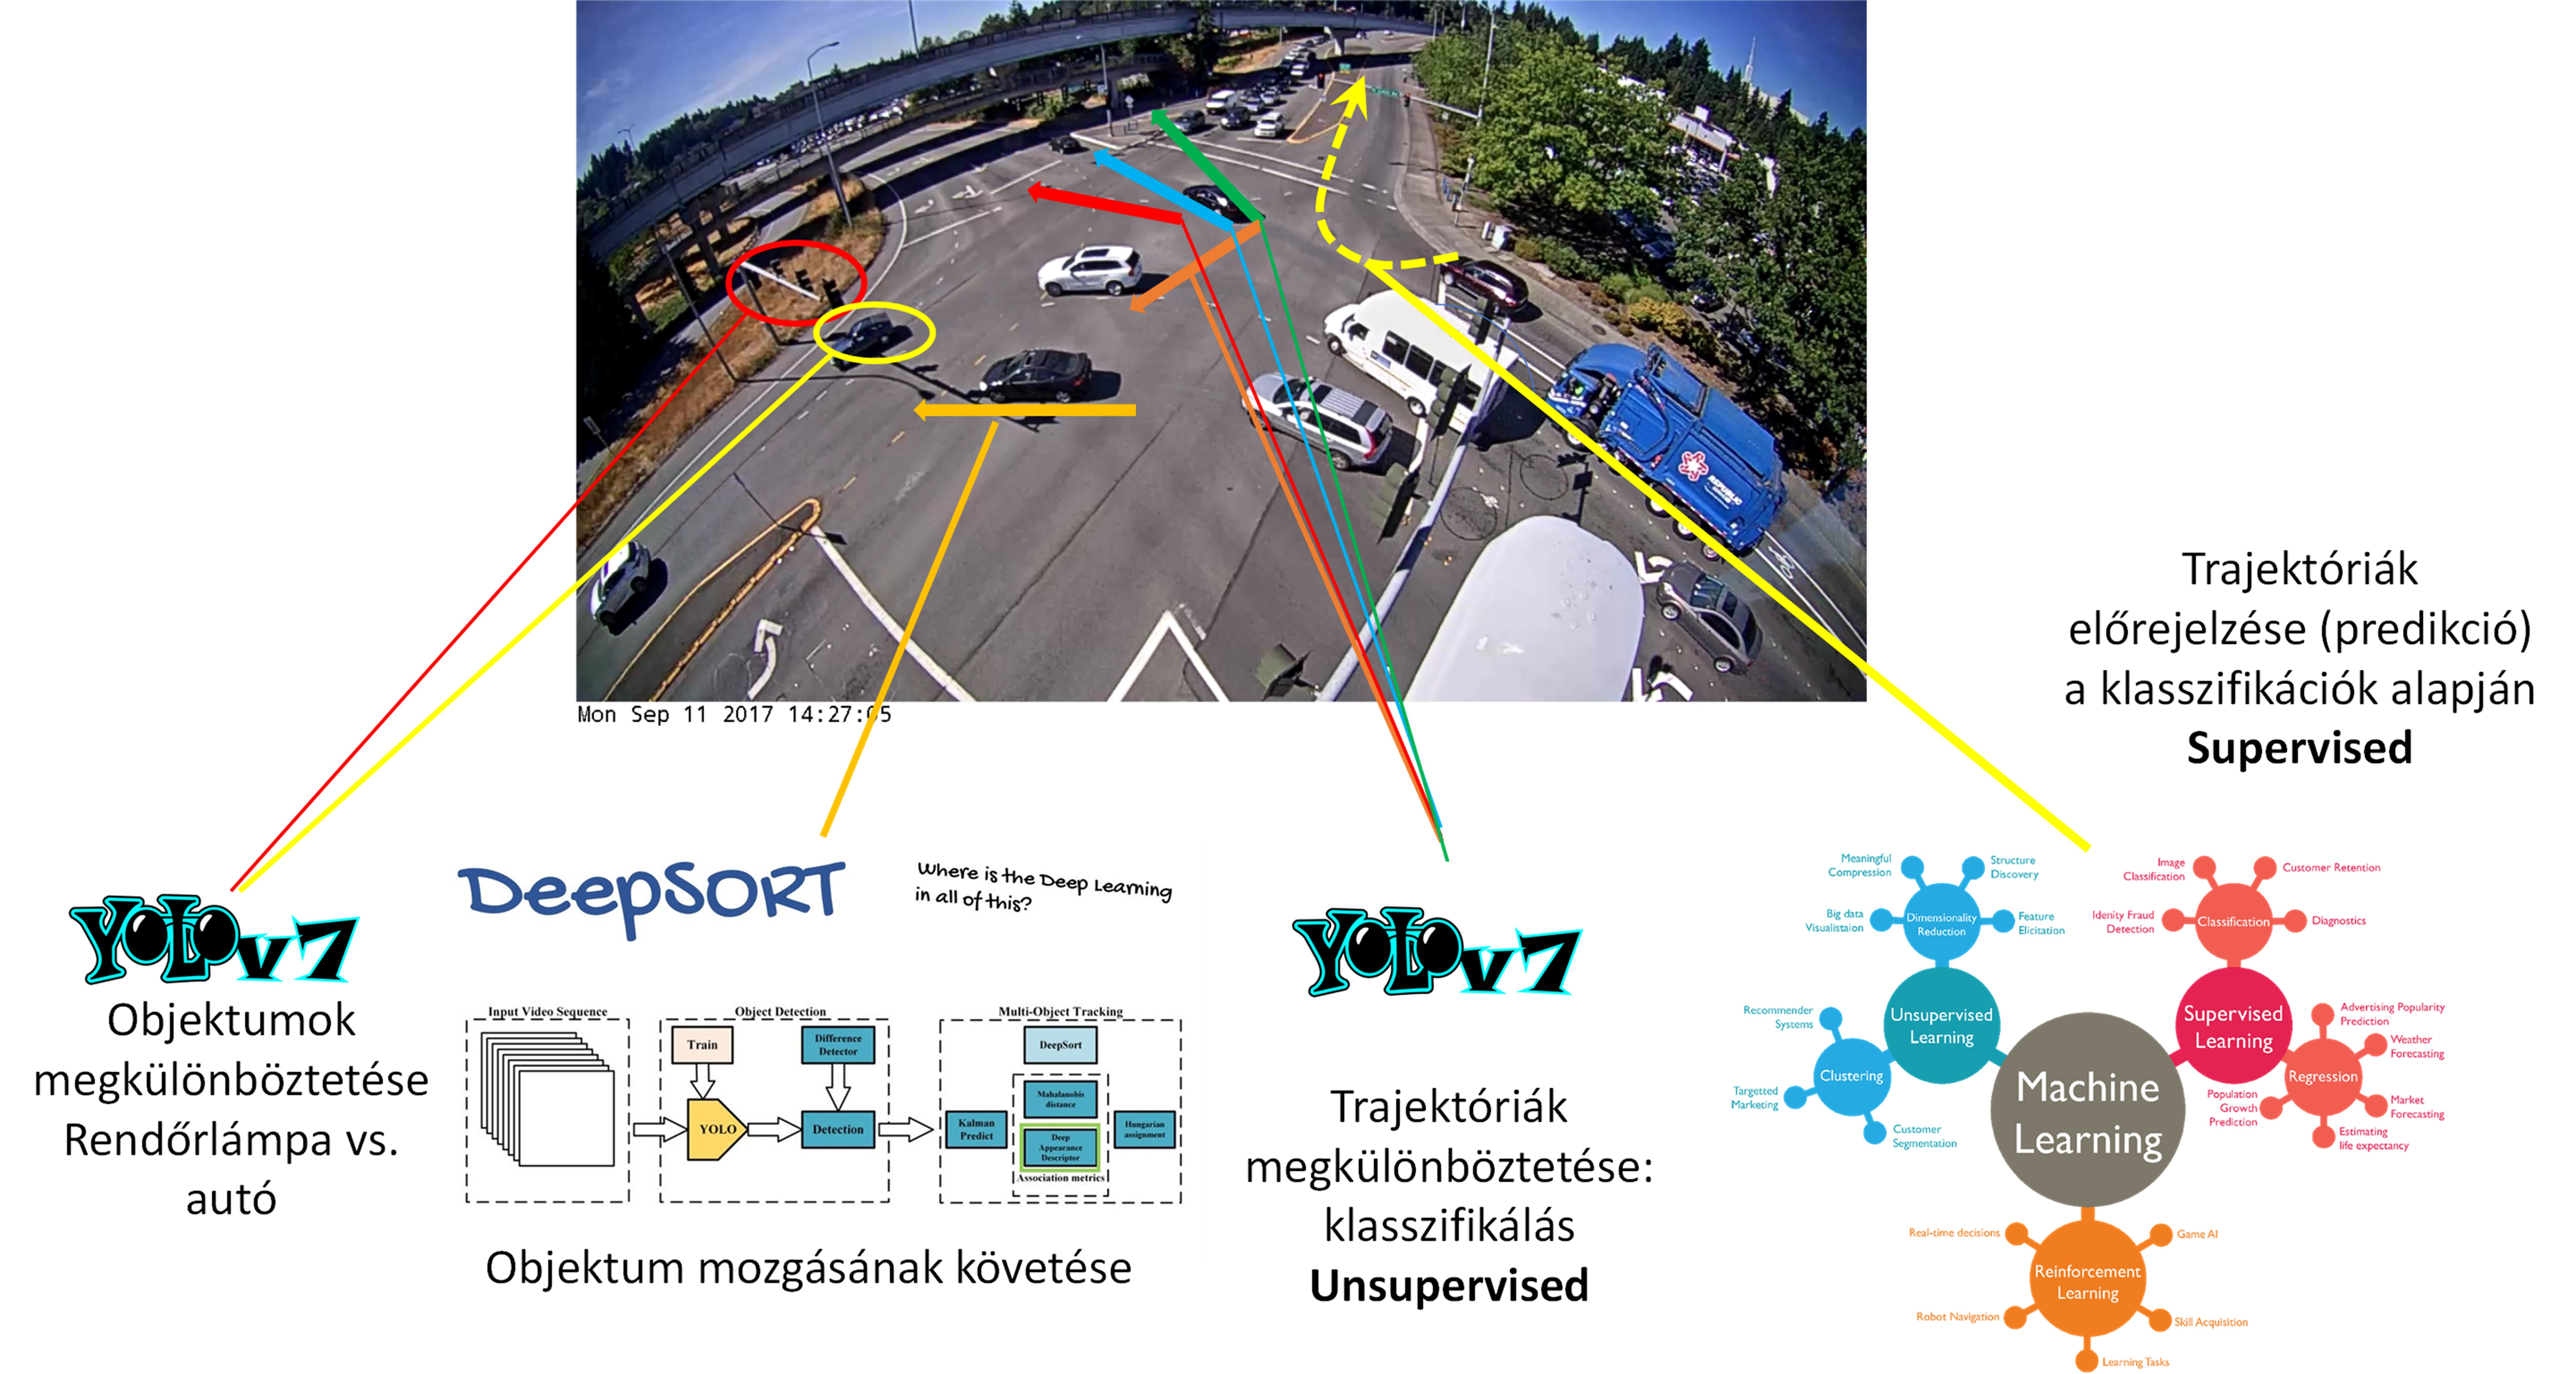
\includegraphics[width=1\columnwidth]{deepsort_yolo_figs/gépilátás_modified.jpg}
%     \caption{Gépi látás}
%     \label{fig: ComputeVision}
% \end{figure}

\paragraph{A tanító adatok} előállításához, objektumok detektálására a YOLOv7 \cite{wang2022yolov7} konvolúciós neurális hálót használtuk, ez a konvolúciós neurális háló architektúra nem csak nagy pontosságot, hanem sebességet is nyújt nekünk. 
Emellett képkockáról képkockára követni is kell tudni a detektált objektumokat. Erre is sok megoldás található manapság, erre a feladatra
a DeepSORT \cite{Wojke2018deep} nevezetű algoritmust használtuk, ez kálmán filtert és konvolúciós neurális hálót használ az objektumok követésére.
A tanító adatok 5 különböző helyszín forgalmát tartalmazzák. Minden helyszín más tulajdonságokkal bír, ezért nem lehet generalizálni
a tanítási folyamatot, nem lehet egy univerzális modellt betanítani ami minden közlekedési helyszínre alkalmazható egyaránt.
4 videót Bellevue város github oldaláról gyűjtöttük, amiknek az elérhetőségét függelékként csatoljuk, a kereszteződések 
\ref{fig: BellevueNewport}. \ref{fig: BellevueEastgate}. \ref{fig: BellevueNE}. \ref{fig: BellevueSE}. képeken láthatók, az ötödik videó La Grange-ból származik lásd \ref{lagrangekynorth}. A videók pontos elérhetőségét
a mellékletben található \emph{urls.txt}-ben adtuk meg.
\begin{figure}
    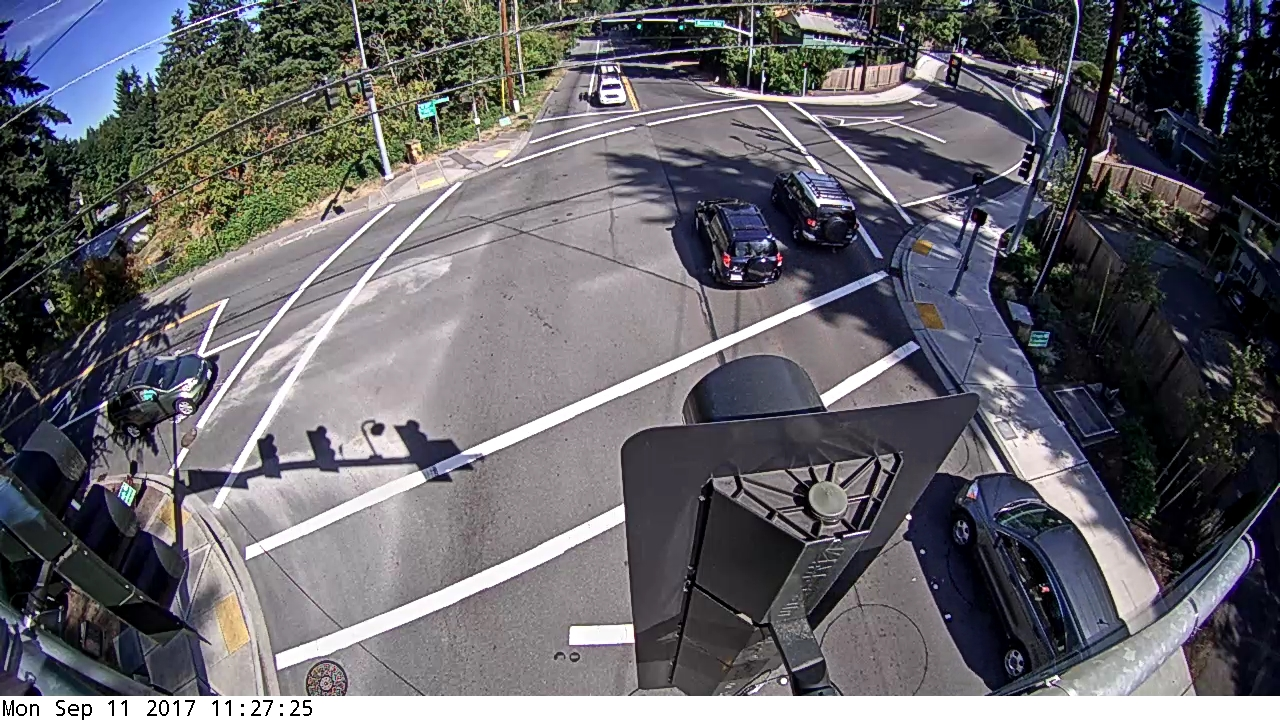
\includegraphics[width=1\columnwidth]{dataset_samples/Bellevue_150th_Newport.JPG}
    \caption{Bellevue Newport kereszteződés}
    \label{fig: BellevueNewport}
\end{figure}
\begin{figure}
    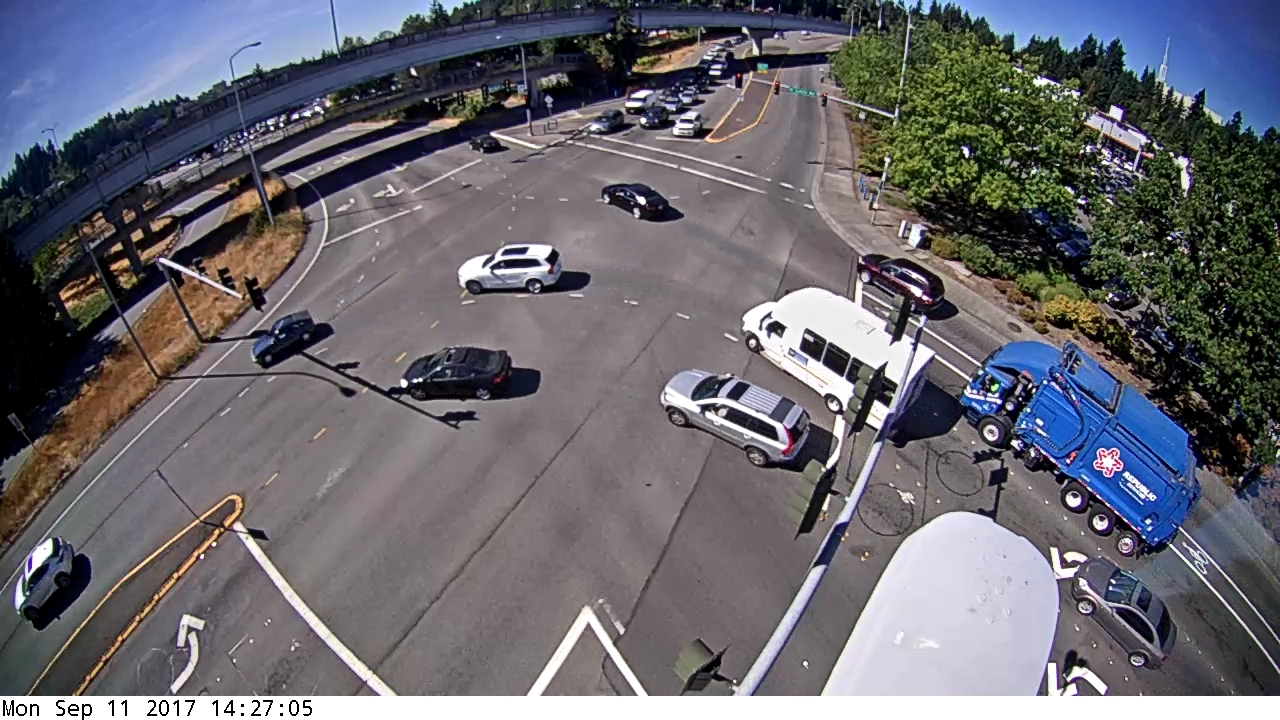
\includegraphics[width=1\columnwidth]{dataset_samples/Bellevue_150th_Eastgate.JPG}
    \caption{Bellevue Eastgate kereszteződés}
    \label{fig: BellevueEastgate}
\end{figure}
\begin{figure}
    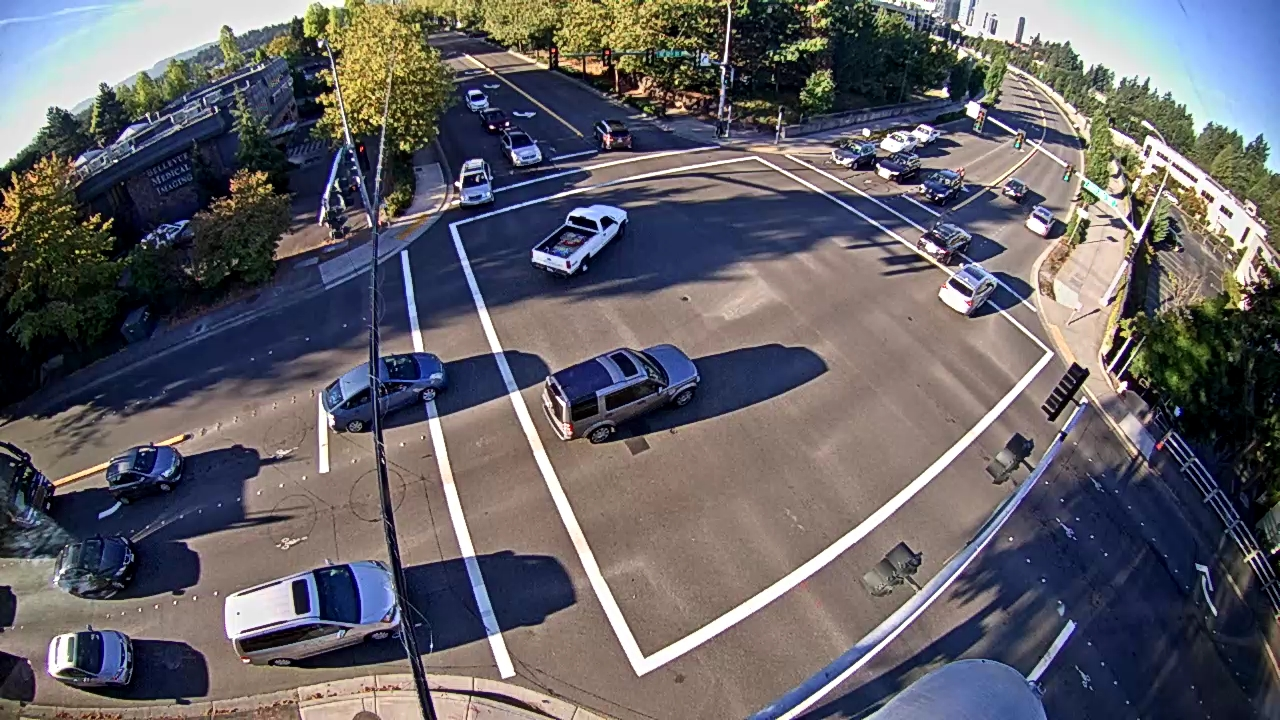
\includegraphics[width=1\columnwidth]{dataset_samples/Bellevue_116th_NE12th.JPG}
    \caption{Bellevue NE kereszteződés}
    \label{fig: BellevueNE}
\end{figure}
\begin{figure}
    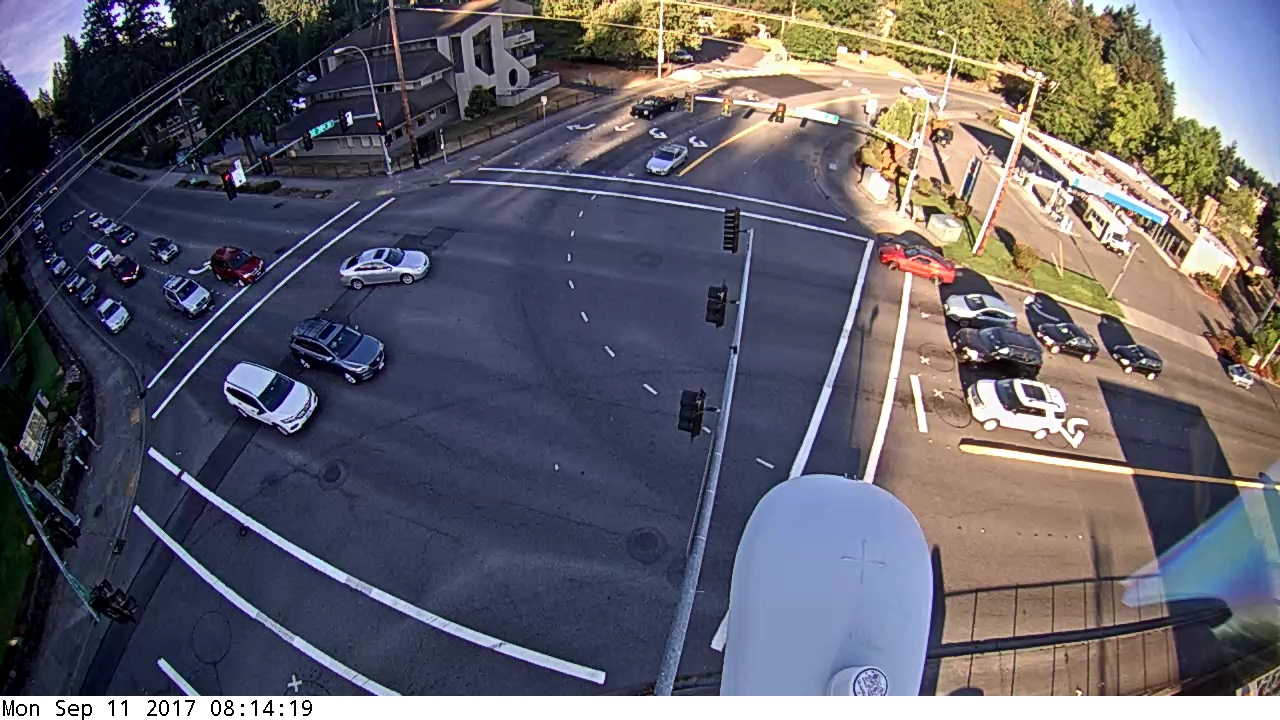
\includegraphics[width=1\columnwidth]{dataset_samples/Bellevue_150th_SE38th.JPG}
    \caption{Bellevue SE kereszteződés}
    \label{fig: BellevueSE}
\end{figure}
\begin{figure}
    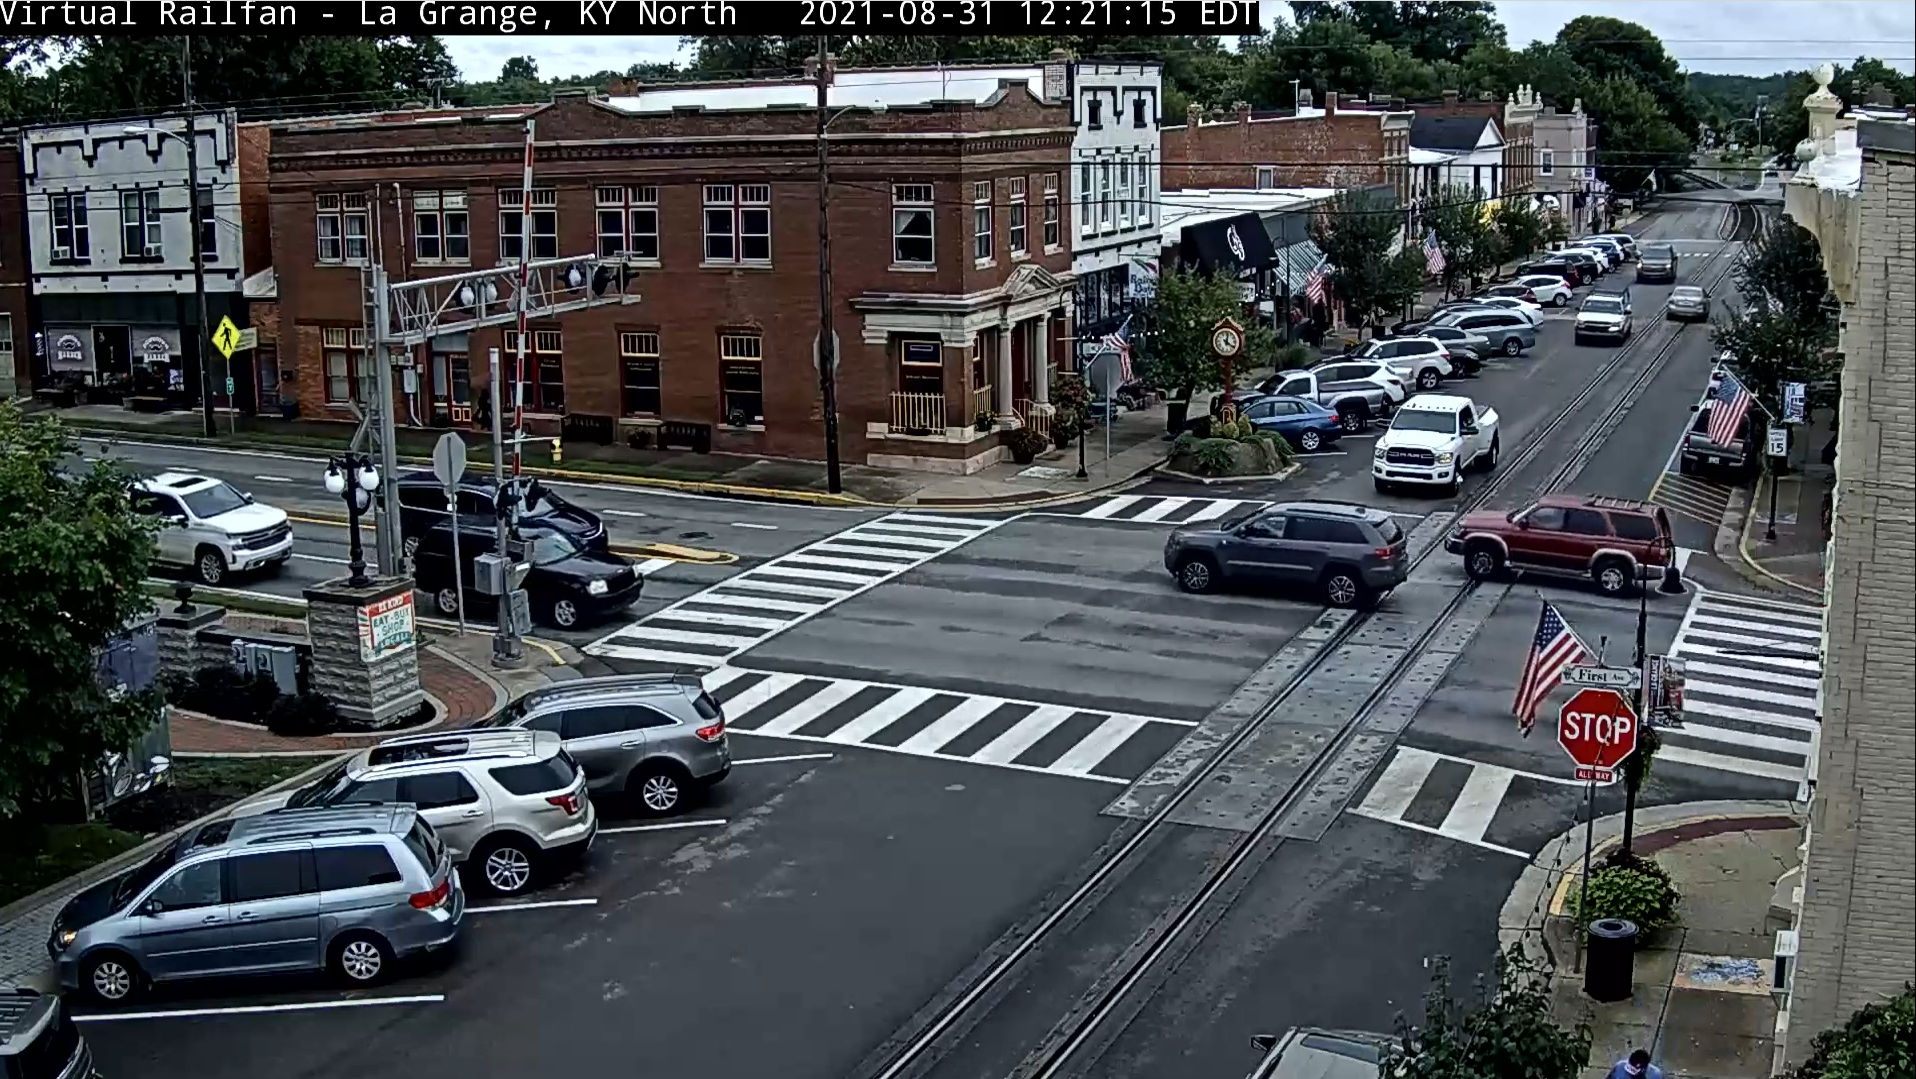
\includegraphics[width=1\columnwidth]{dataset_samples/lagrange_kynorth.png}
    \caption{La Grange KY North}
    \label{lagrangekynorth}
\end{figure}

\newpage
\section{Kapcsolódó kutatások}
Sok ITS-el kapcsolatos kutatásban tárgyalják a forgalom folyás (traffic flow) előrejelzését. \cite{PAUL2017177} összehasonlítja az eddig
kutatott és használt modellek, mint például Kálmán-szűrő, k-nearest neighbor (k-NN), mesterséges neurális hálók, stb., pontosságát és
sebességét, ezen modellek továbbkutatását, mivel egyre növekednek a különböző szenzorok által  begyűjtött traffic flow adatok, így ez a terület belépett
a \emph{Big Data} korszakába. \cite{10.1371/journal.pone.0253868} is a traffic flow előrejelzését és generálását tárgyalja, Floating Car Data (FCD) 
adathalmazokon betanított, Hosszú-Rövid-Távú memóriájú és Generatív versengő hálókkal.
\newpage
\subsection{YOLO}
YOLO (You Only Look Once) egy nagyon hatékony objektumdetektáló algoritmus, amely képes nagyon gyorsan észlelni és besorolni az objektumokat egy képen vagy videón.
A YOLO algoritmus működése a következő lépésekből áll:
\begin{enumerate}
    \item Bemeneti kép előkészítése: A kép előkészítése magában foglalja a normalizálást és a méretarányhoz való igazítást annak érdekében, hogy az YOLO algoritmus hatékonyan dolgozhasson a képpel.
    \item Vektor előállítása: A YOLO algoritmus a bemeneti képet a vektorizálás segítségével elemzi, amelynek eredménye egy tensor lesz, amely az objektumok lokalizációjához és azok osztályozásához szükséges információkat tartalmazza.
    \item Konvolúciós hálózat alkalmazása: A YOLO algoritmus egy kiterjedt konvolúciós hálózatot alkalmaz a vektorra, amelynek célja az objektumok lokalizálása és azok osztályozása.
    \item Konvolúciós hálózat alkalmazása: A YOLO algoritmus egy kiterjedt konvolúciós hálózatot alkalmaz a vektorra, amelynek célja az objektumok lokalizálása és azok osztályozása.
    \item Objektum lokalizálása és osztályozása: A YOLO algoritmus az általa előállított tenzoron keresztül végzi az objektumok lokalizálását és azok osztályozását. Az algoritmus meghatározza az objektumok koordinátáit és a hozzájuk tartozó osztályt.
\end{enumerate}
A YOLO algoritmus előnye, hogy nagyon gyors és hatékonyan kezeli az objektumok lokalizálását és azok osztályozását. Az algoritmus gyakran jobb teljesítményt nyújt, mint a hasonló módszerek, és a különböző objektumokat a bemeneti képen gyorsan és hatékonyan azonosítja. Azonban az YOLO algoritmus hibázhat, ha az objektumok nagyon hasonlóak egymáshoz vagy a háttérhez, és nagyobb hibát eredményezhet, ha az objektumok nagyon kicsik a képen.
Legfrissebb változata a Yolov7 felülmúlja sebességben és pontosságban a modern konvolúciós hálókat (lásd \ref{fig: Yolov3chart} \ref{fig: Yolov4chart} \ref{fig: Yolov7chart}). Beágyazott rendszerekben és videókártyákon is egyaránt jó a teljesítménye, ezért az ITS területén alkalmazható. 
\begin{figure}[H]
 \begin{description}
    \centering
    \item[YOLOv3 perfomance over other CNN models.] 
 \end{description}
 \centering
 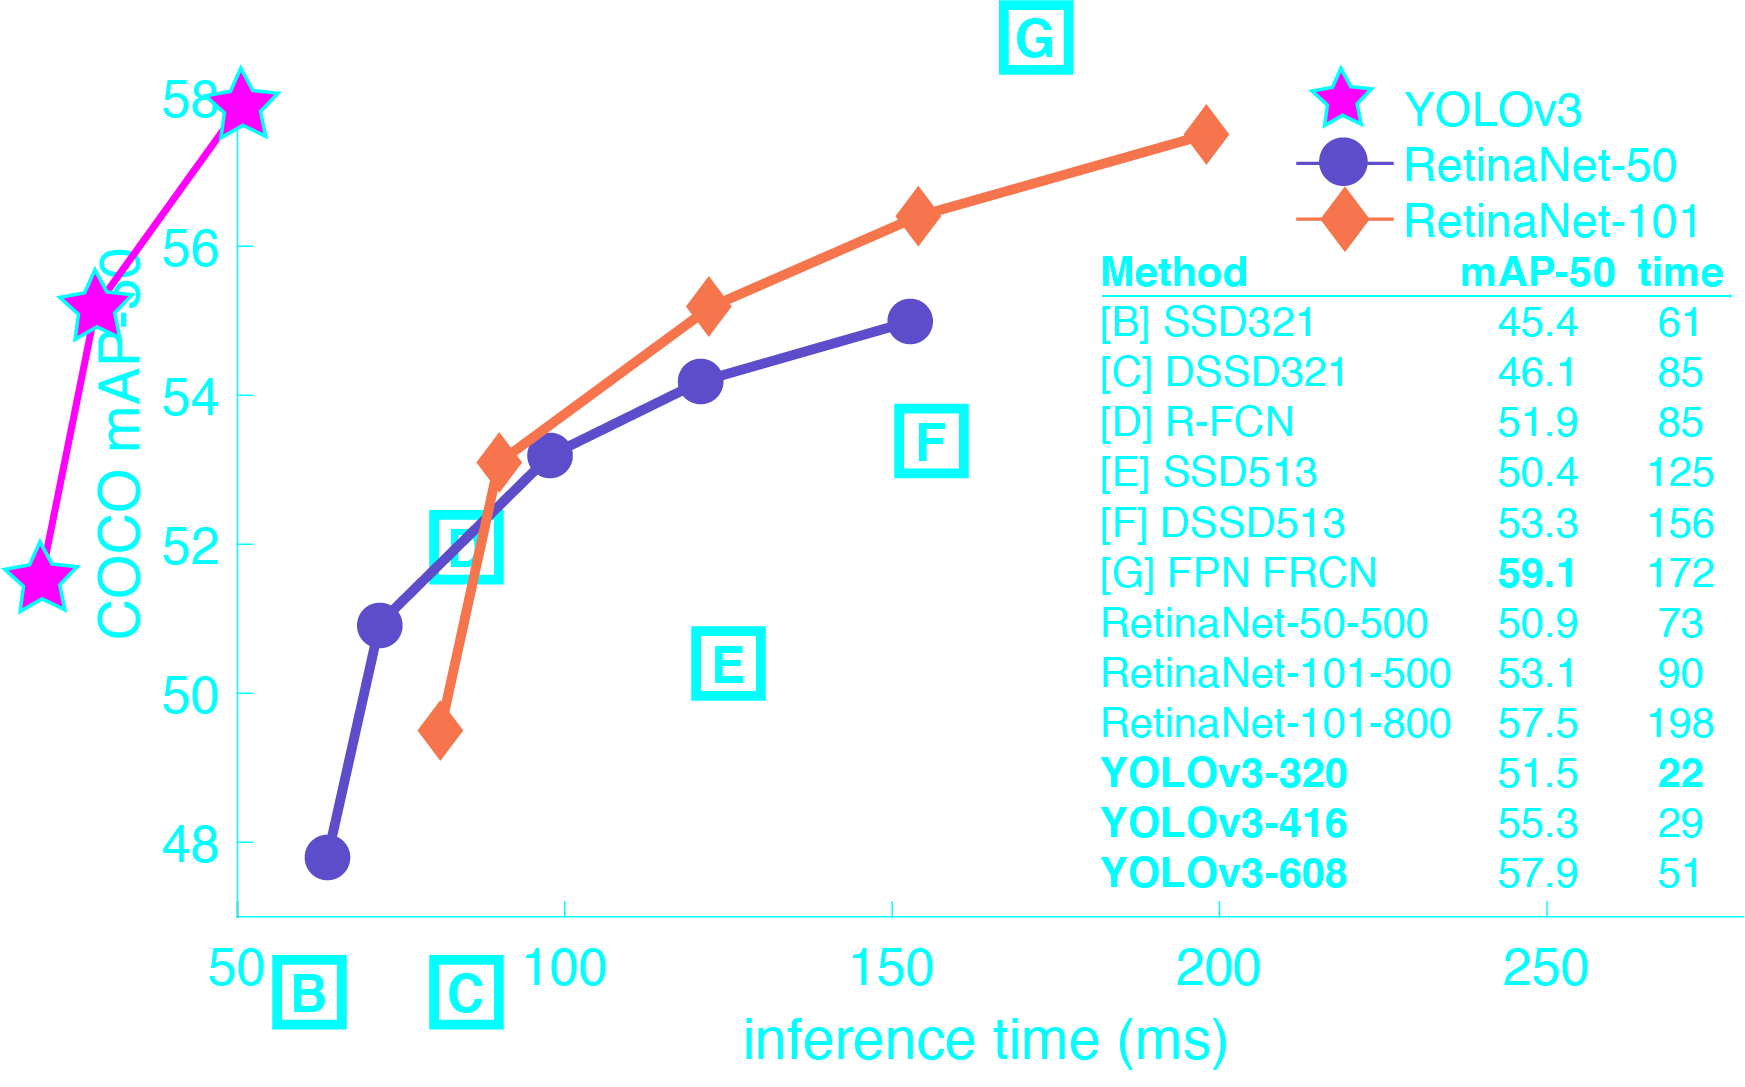
\includegraphics[width=0.6\columnwidth]{yolov3_perf.png}
 \caption{YOLOv3 Performance}
 \label{fig: Yolov3chart}
\end{figure}
\begin{figure}[H]
 \begin{description}
    \centering
    \item[YOLOv4 perfomance over other CNN models.] 
 \end{description}
 \centering
 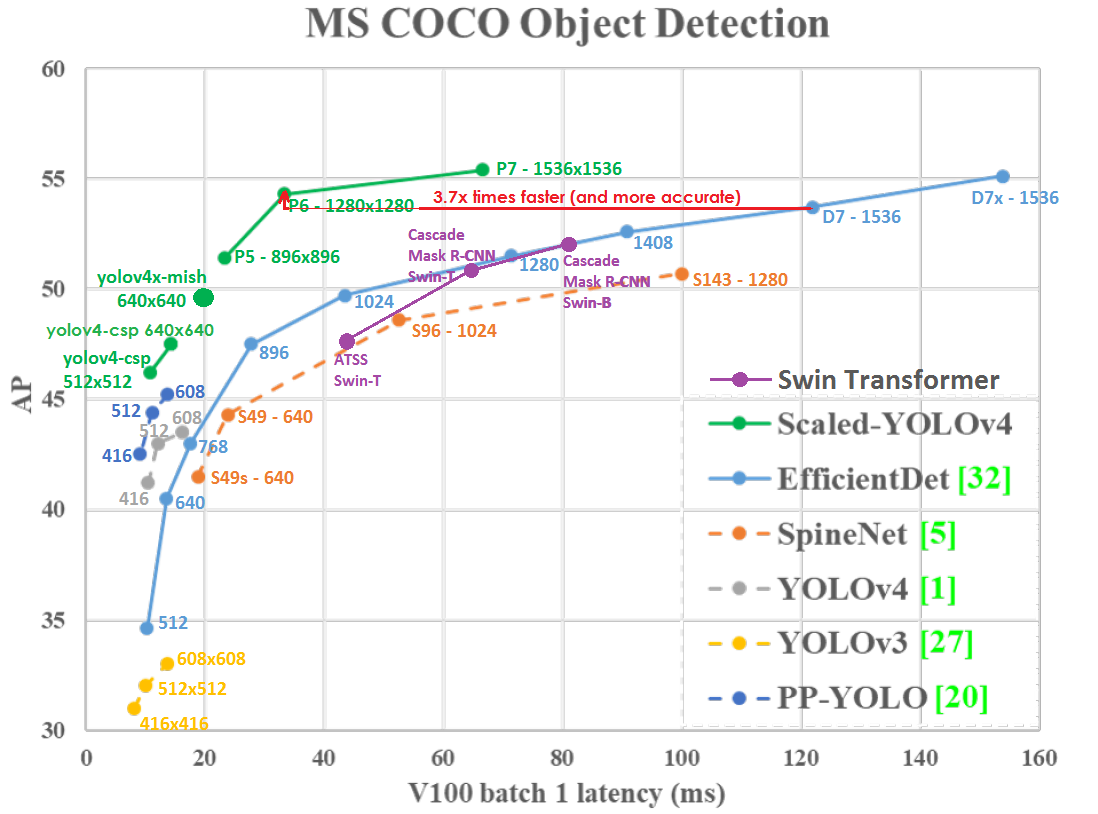
\includegraphics[width=0.6\columnwidth]{yolov4_perf.png}
 \caption{YOLOv4 Performance}
 \label{fig: Yolov4chart}
\end{figure}
\begin{figure}[H]
 \begin{description}
    \item[YOLOv7 perfomance over other yolo models.] 
 \end{description}
 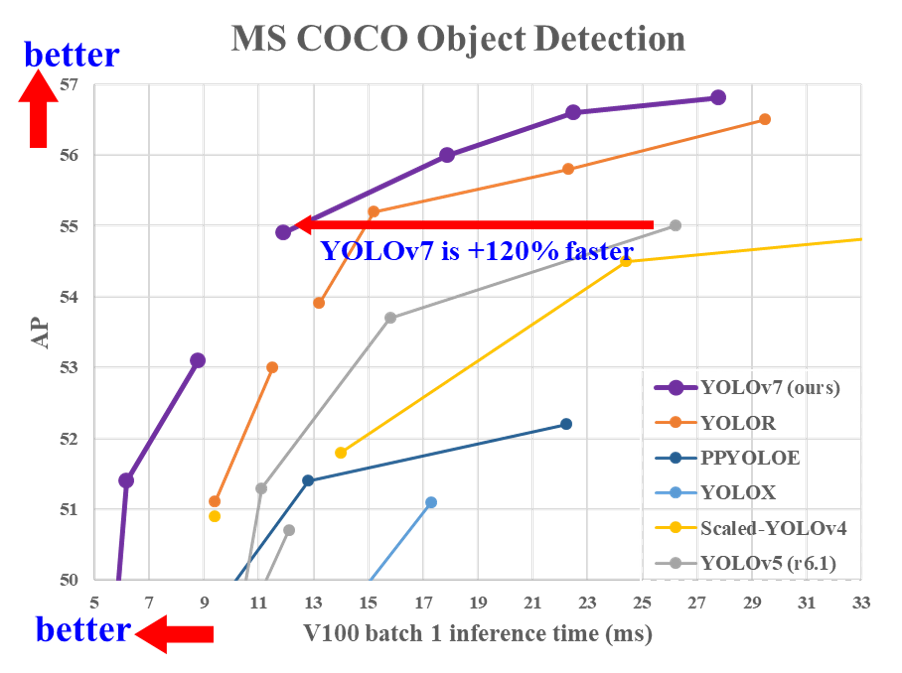
\includegraphics[width=1\columnwidth]{performance.png}
 \caption{YOLOv7 Performance}
 \label{fig: Yolov7chart}
\end{figure}
\subsection{DeepSORT}
A YOLO algoritmus előnye, hogy nagyon gyors és hatékonyan kezeli az objektumok lokalizálását és azok osztályozását. Az algoritmus gyakran jobb teljesítményt nyújt, mint a hasonló módszerek, és a különböző objektumokat a bemeneti képen gyorsan és hatékonyan azonosítja. Azonban az YOLO algoritmus hibázhat, ha az objektumok nagyon hasonlóak egymáshoz vagy a háttérhez, és nagyobb hibát eredményezhet, ha az objektumok nagyon kicsik a képen.
A DeepSORT algoritmus működése a következő lépésekből áll:
\begin{enumerate}
    \item Objektumdetektálás: Az algoritmus először objektumdetektálással azonosítja az összes objektumot a videófelvételen, például a YOLO objektumdetektáló algoritmust használva.
    \item Jellemzők kinyerése: A DeepSORT az objektumok jellemzőit (pl. méret, sebesség, szín) kinyeri, hogy a következő lépésben a következő objektumot azonosítani tudja.
    \item Objektumazonosítás: Az algoritmus használ egy "tracklet" nevű algoritmust, hogy azonosítsa és kövesse az objektumokat az időben. A "tracklet" az objektum jellemzőit használja, hogy azonosítsa az adott objektumot a videófelvétel további részein.
    \item Címkézés: Az objektumokat azonosítják egyedi azonosítókkal, hogy az algoritmus megkülönböztethesse azokat az egyes videófelvételeken.
    \item Korszakosítás: A DeepSORT algoritmus általánosan a Kálmán-szűrőt használja, amely folyamatosan frissíti az objektumok helyzetének becslését. A Kálmán-szűrő segít az algoritmusnak megjósolni az objektumok további helyzetét a videófelvétel során.
\end{enumerate}
A DeepSORT algoritmus előnye, hogy nagyon stabil és pontos objektumkövetést biztosít akkor is, ha az objektumok átmennek más objektumok mögött vagy ha azok mozgása elég bonyolult. Az algoritmus nagyobb pontosságot nyújt a hagyományos objektumkövetési algoritmusokhoz képest, és képes megbirkózni a nagy sebességű objektumok követésével is. Azonban az algoritmus nagyobb számítási erőforrásokat igényel, és magasabb szintű számítási készséget igényel az implementáláshoz.
\begin{figure}
    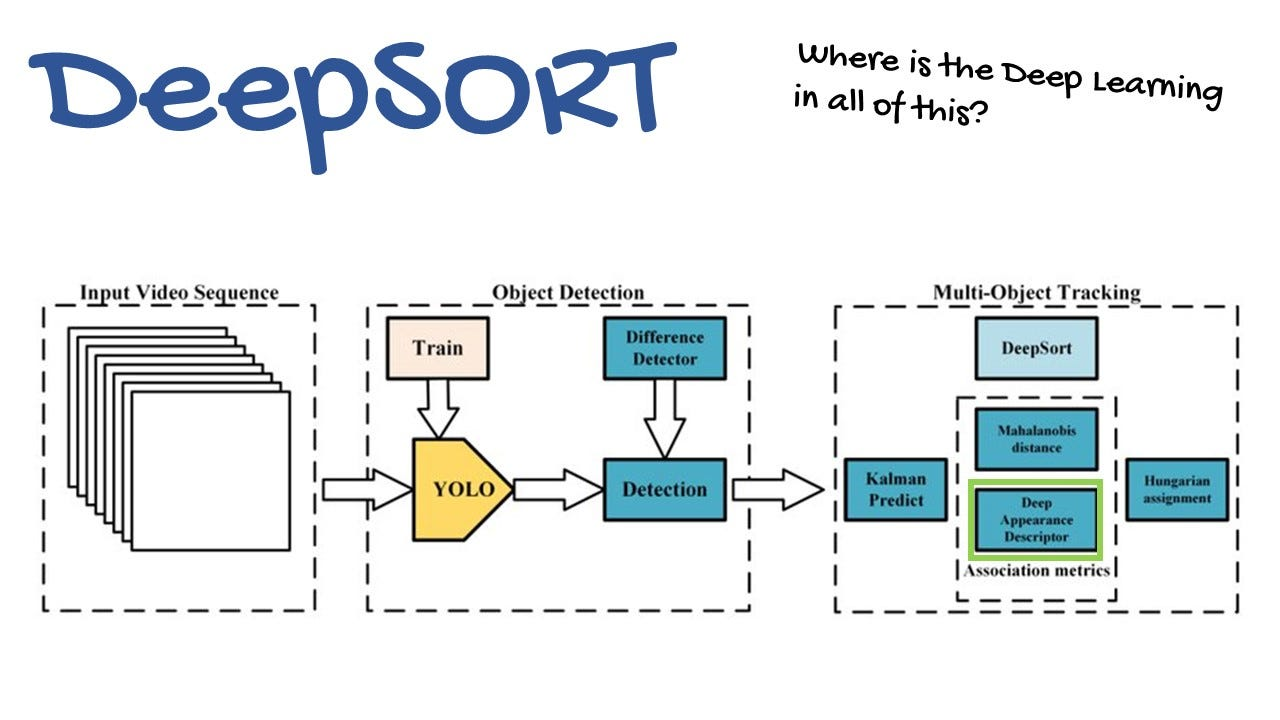
\includegraphics[width=1\columnwidth]{deepsort_yolo_figs/deepsort_block_diagram.jpg}
    \caption{Objektum követés}
    \label{ObjectTracking}
\end{figure}

\newpage
\section{Adathalmazok kialakítása}
A kutatás során saját adathalmazok kialakítására volt szükség. Az adatok begyűjtésére és eltárolására saját alkalmazást és keretrendszert
fejlesztettünk ki. A szoftver keretrendszert python nyelven írtuk meg, a forráskód ezen a linken megtatlálható \url{http://github.com/Pecneb/computer_vision_research}.
A fejlesztés során a következő programkönyvtárakat használtuk OpenCV \cite{opencv_library}, Numpy \cite{harris2020array}, Pandas \cite{reback2020pandas}, 
Scikit-Learn \cite{scikit-learn}, Matplotlib \cite{Hunter:2007}, SQLite \cite{sqlite2020hipp}, Joblib \cite{joblib_library}. Az adathalmazokat SQLite adatbázisban és
joblib fájlokban tároltuk el. Azért döntöttünk így, hogy két féle módon is eltároljuk az adathalmazokat, mert az SQL adatbázist univerzálisan
bármilyen adatbáziskezelővel, vagy más programnyelvvel be lehet olvasni, viszont a joblib fájlokat sokkal gyorsabban be lehet töletni pythonnal.

\newpage
\subsection{Adatstruktúra}
Az adatstruktúrát SQL schema-ként, és python osztály-ként is definiáltuk.
\begin{minted}{sql}
CREATE TABLE IF NOT EXISTS objects (
            objID INTEGER PRIMARY KEY NOT NULL,
            label TEXT NOT NULL
        );
CREATE TABLE IF NOT EXISTS detections (
            objID INTEGER NOT NULL,
            frameNum INTEGER NOT NULL,
            confidence REAL NOT NULL,
            x REAL NOT NULL,
            y REAL NOT NULL,
            width REAL NOT NULL,
            height REAL NOT NULL,
            vx REAL NOT NULL,
            vy REAL NOT NULL,
            ax REAL NOT NULL,
            ay REAL NOT NULL,
            vx_c REAL NOT NULL,
            vy_c REAL NOT NULL,
            ax_c REAL NOT NULL,
            ay_c REAL NOT NULL,
            FOREIGN KEY(objID) REFERENCES objects(objID)
        );
CREATE TABLE IF NOT EXISTS metadata (
            historyDepth INTEGER NOT NULL,
            yoloVersion TEXT NOT NULL,   
            device TEXT NOT NULL,
            imgsize INTEGER NOT NULL,
            stride INTEGER NOT NULL,
            confidence_threshold REAL NOT NULL,
            iou_threshold REAL NOT NULL,
            k_velocity REAL NOT NULL,
            k_acceleration REAL NOT NULL
        );
\end{minted}
Minden követett objektum egyedi azonosítóval lett ellátva. Az objektumhoz tartozó detektálások külön táblába lettek kiszervezve,
ahol az \textit{objID} idegen kulccsal kapcsoljuk az \textit{objektumok} táblához. Egy objektumhoz az egyedi azonosítón kívül
tartozik egy \textit{label}, amit a YOLO objektum detektálótól kap, ez lehet pl. autó, személy, teherautó, stb. Az objektumokhoz
tartózó detektálások tartalmazzák a képkocka számát, amikor a detektálás történt, a konfidenciát, hogy mennyire biztos az
objektumfelismerő a hozzárendelt \textit{label}-ben, az objektum \begin{math}x,y\end{math} koordinátáját, az objektum szélességét
\begin{math}width\end{math} és magasságát \begin{math}width\end{math}, sebességét \begin{math}v_x,v_y\end{math} és gyorsulását \begin{math}a_x,a_y\end{math}, 
amik a deepSORT által kalkulált értékek, így még külön a koordinátákból kiszámolt \begin{math}v_{x_c},v_{y_c}\end{math} sebességet és
\begin{math}a_{x_c},a_{y_c}\end{math} gyorsulást is eltároltuk.
Ezek mellett még a konfigurációs adatokat is külön táblában tároljuk, hogy később meg lehessen ismételni a detektálást. 
A koordinátákat a videó méretének megfelelően leskálázzuk 0 - 1 értékek köré. Ha a videókép szélesség \begin{math}w\end{math}, magasság \begin{math}h\end{math}, 
akkor a képarány \begin{math}r = \frac{w}{h}\end{math}, és az eltárolt koordináták 
\begin{equation}x = \frac{x_0}{w} \cdot r, y = \frac{y_0}{w} \cdot r\end{equation}
\begin{equation}v_x = \frac{v_{x_0}}{w} \cdot r, v_y = \frac{v_{y_0}}{w} \cdot r\end{equation}
\begin{equation}a_x = \frac{a_{x_0}}{w} \cdot r, a_y = \frac{a_{y_0}}{w} \cdot r\end{equation}
\begin{equation}v_{x_c} = \frac{v_{xc0}}{w} \cdot r, v_{y_c} = \frac{v_{yc0}}{w} \cdot r\end{equation}
\begin{equation}a_{x_c} = \frac{a_{xc0}}{w} \cdot r, a_{y_c} = \frac{a_{yc0}}{w} \cdot r\end{equation}.

\newpage
\subsection{Objektumdetektálás}
Az objektumdetektáláshoz a fent említett YOLO modellt haszáltuk. Kutatásunk kezdetekor, a YOLO 4-es verziójával kezdtünk dolgozni,
de később átváltottunk a jobb pontosságot és sebességet ígérő 7-es verzióra.
\subsubsection{YOLOv4}
YOLO 4-es verzióját, C-ben implementálták. Hogy fel tudjuk használni, írnunk kellett egy python API-t, amit meg tudtunk hívni a
detektáló programunkban.
\subsubsection{YOLOv7}
A YOLOv7 viszont már python-ban implementálták, amihez már sokkal könnyebb volt API-t programozni és használni. Emellett gyorsaságban
és pontosságban is felülmúlta a 4-es verziót (lásd \ref{fig: Yolov7chart}).
\subsection{Objektumkövetés}
Ahhoz, hogy trajektóriák alapján tudjunk szabályosságokat felismerni a forgalomban, pontos objektumkövetésre volt szükségünk. Eleinte
saját objektumkövető algoritmust használtunk, ami deketálások euklideszi távolsága alapján próbálta meg követni az objektumokat.
Ezzel az volt a gond, hogy hosszabb kitakarás után nem találta meg az objektumot, így egy új objektumnak számított, ami a kép
közepéből bukkant fel. Ennek a problémának a kiküszöbölésére próbáltuk ki a DeepSORT algoritmust.
\subsubsection{DeepSORT}
A DeepSORT algoritmus pythonban implementált változatát integráltuk a mi programunkba.

\newpage
\section{Klaszterezés}
A klaszterezés segítségével lehet az adathalmazból alőállítani a klasszifikáció alapjául szolgáló klasszokat. Ahhoz, hogy az
a rengeteg trajektóriából és detektálásból számunkra felhasználható információ keletkezzen, meg kell határoznunk feature
vectorokat, amik a trajektóriákra jellemző értékeket tartalmaznak. Ebben a feature térben fogja a klaszterező algoritmus
megtalálni az egymáshoz közeli, hasonló trajektóriákat.
\subsection{Adattisztítás}
A klaszterezés előtt a nyers adatokat fel kell dolgoznunk, hogy az esetleges hibás, zajos detektálások, trajektóriák miatt
kapjunk fals klasztereket. Az objektum detektálás és követés nem tökéletes, rossz fényviszonyok, hosszabb eltakarások miatt 
a trajektóriák megszakadhatnak, ezért ki kell választani az egyben maradt trajektóriákat. Három szűrő algoritmust futtattunk 
az adathalmazon. Elsőnek a trajektóriák belépő és kilépő pontjainak az euklideszi távolsága alapján szűrtünk. Ezzel a szűréssel a zajos, félbeszakadt trajektóriákat szűrjük ki.
Majd a kép széleit meghatározzuk min-max kiválasztással, és azokat a trajektóriákat választjuk ki, amiknek a szélektől meghatározott
távolságra vannak a belépő és kilépő pontjaik. Erre azért van szükség, mert ha belegondolunk, lehet hogy a kép egyik szélén valami eltakarja az utat pl. egy ház, és akkor az autók belépési pontjai a kép közepétől indulnak, ami nem jelenti azt, hogy az egy zajos, hibás trajektória, hanem ez a kereszteződés egy sajátossága. 
\subsubsection{DeepSORT pontatlanság}
Kutatásunk során azt tapasztaltuk, hogy a DeepSORT és a YOLO pontatlanságai felerősítik egymást. A YOLO hajlamos néha táblákat
vagy rendőrlámpákat autóknak nézni, és ekkor a DeepSORT is elkezdi követni. Egy olyan hibáját is felfedeztük a DeepSORT-nak, hogy
egy objektumról áttapad a követés egy másik objektumra, ami fals trajektóriákat hoz létre. A DeepSORT-nak lehet finomhangolni a
paramétereit, ami nem bizonyult akkora javulásnak, ezért utólagos szűréssel kellett korrigálnunk ezt a hibát. Az algoritmus végig 
iterál a trajektóriák pontjain és kiszámítja az egymást követő detektálások euklideszi távoláságát, és ha egy küszöbérték felett vannak, akkor eldobjuk a trajektóriát.
A következő képeken láthatók a klaszterek szűrés előtt és után (lásd \ref{fig: Klaszterezés szűrő} \ref{fig: Klaszterezés szűrő2} \ref{fig: Klaszterezés szűrő3}), ahol a bal oldali oszlop reprezentálja a szűrés előtti klasztereket, a jobb oldali oszlop pedig a szűrés utáni klasztereket.

\begin{figure}[H]
 \centering
 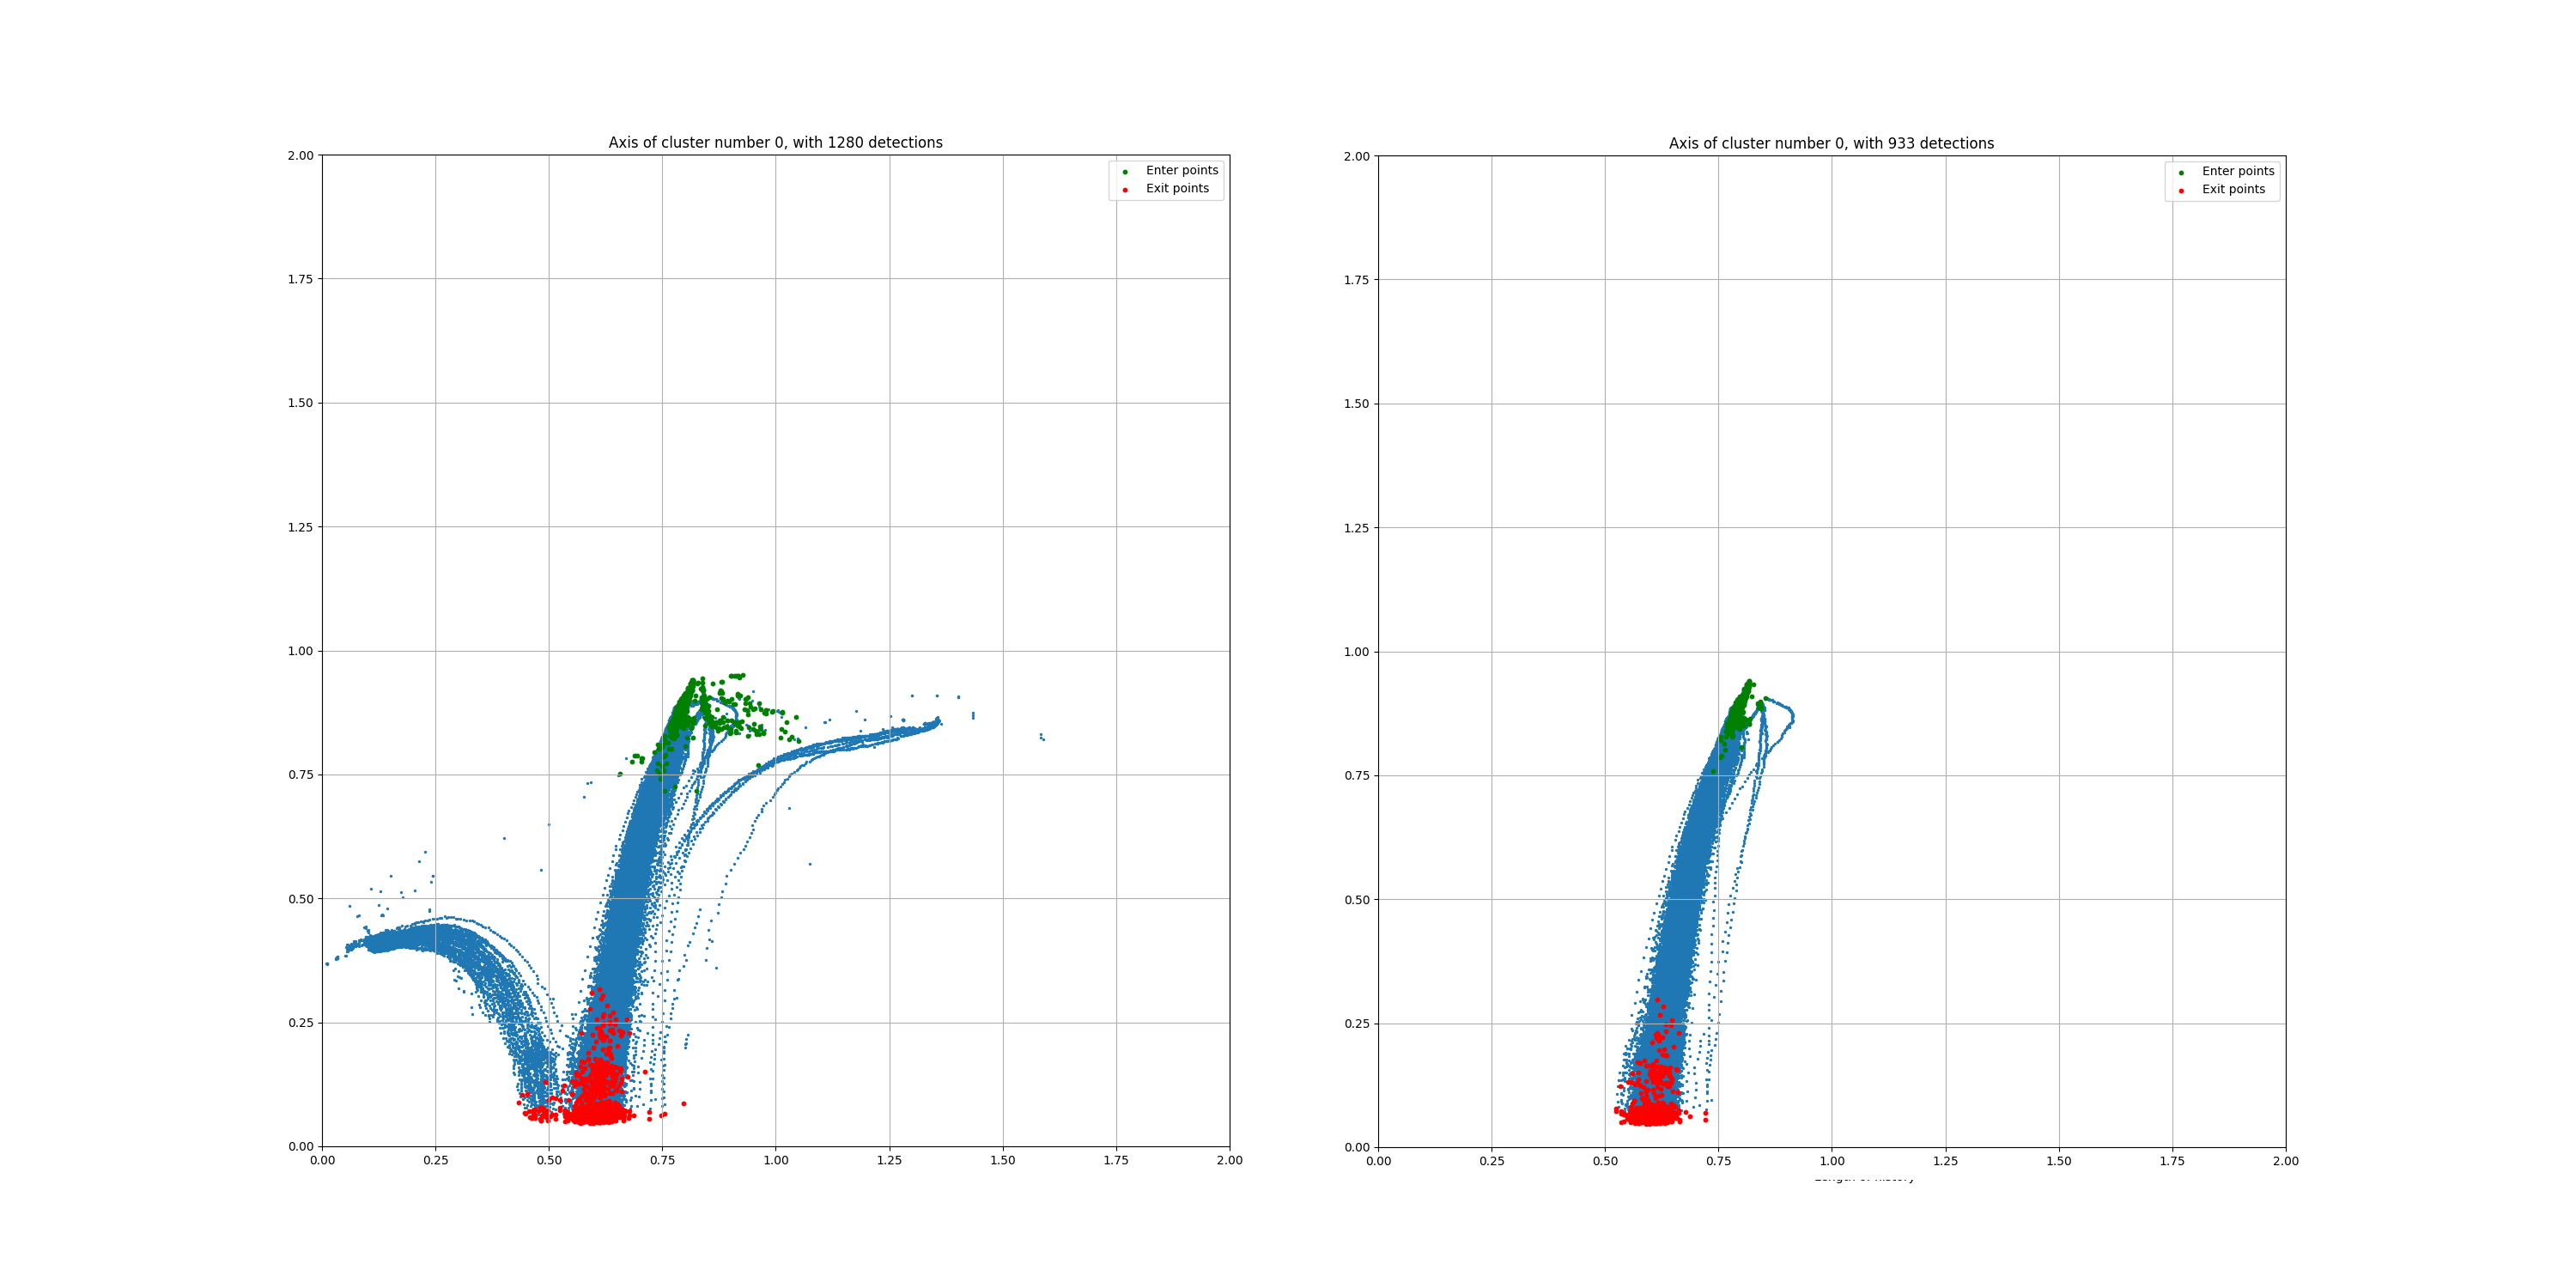
\includegraphics[width=0.8\columnwidth]{clustering/n_cluster_0_before_after.png}
 \centering
 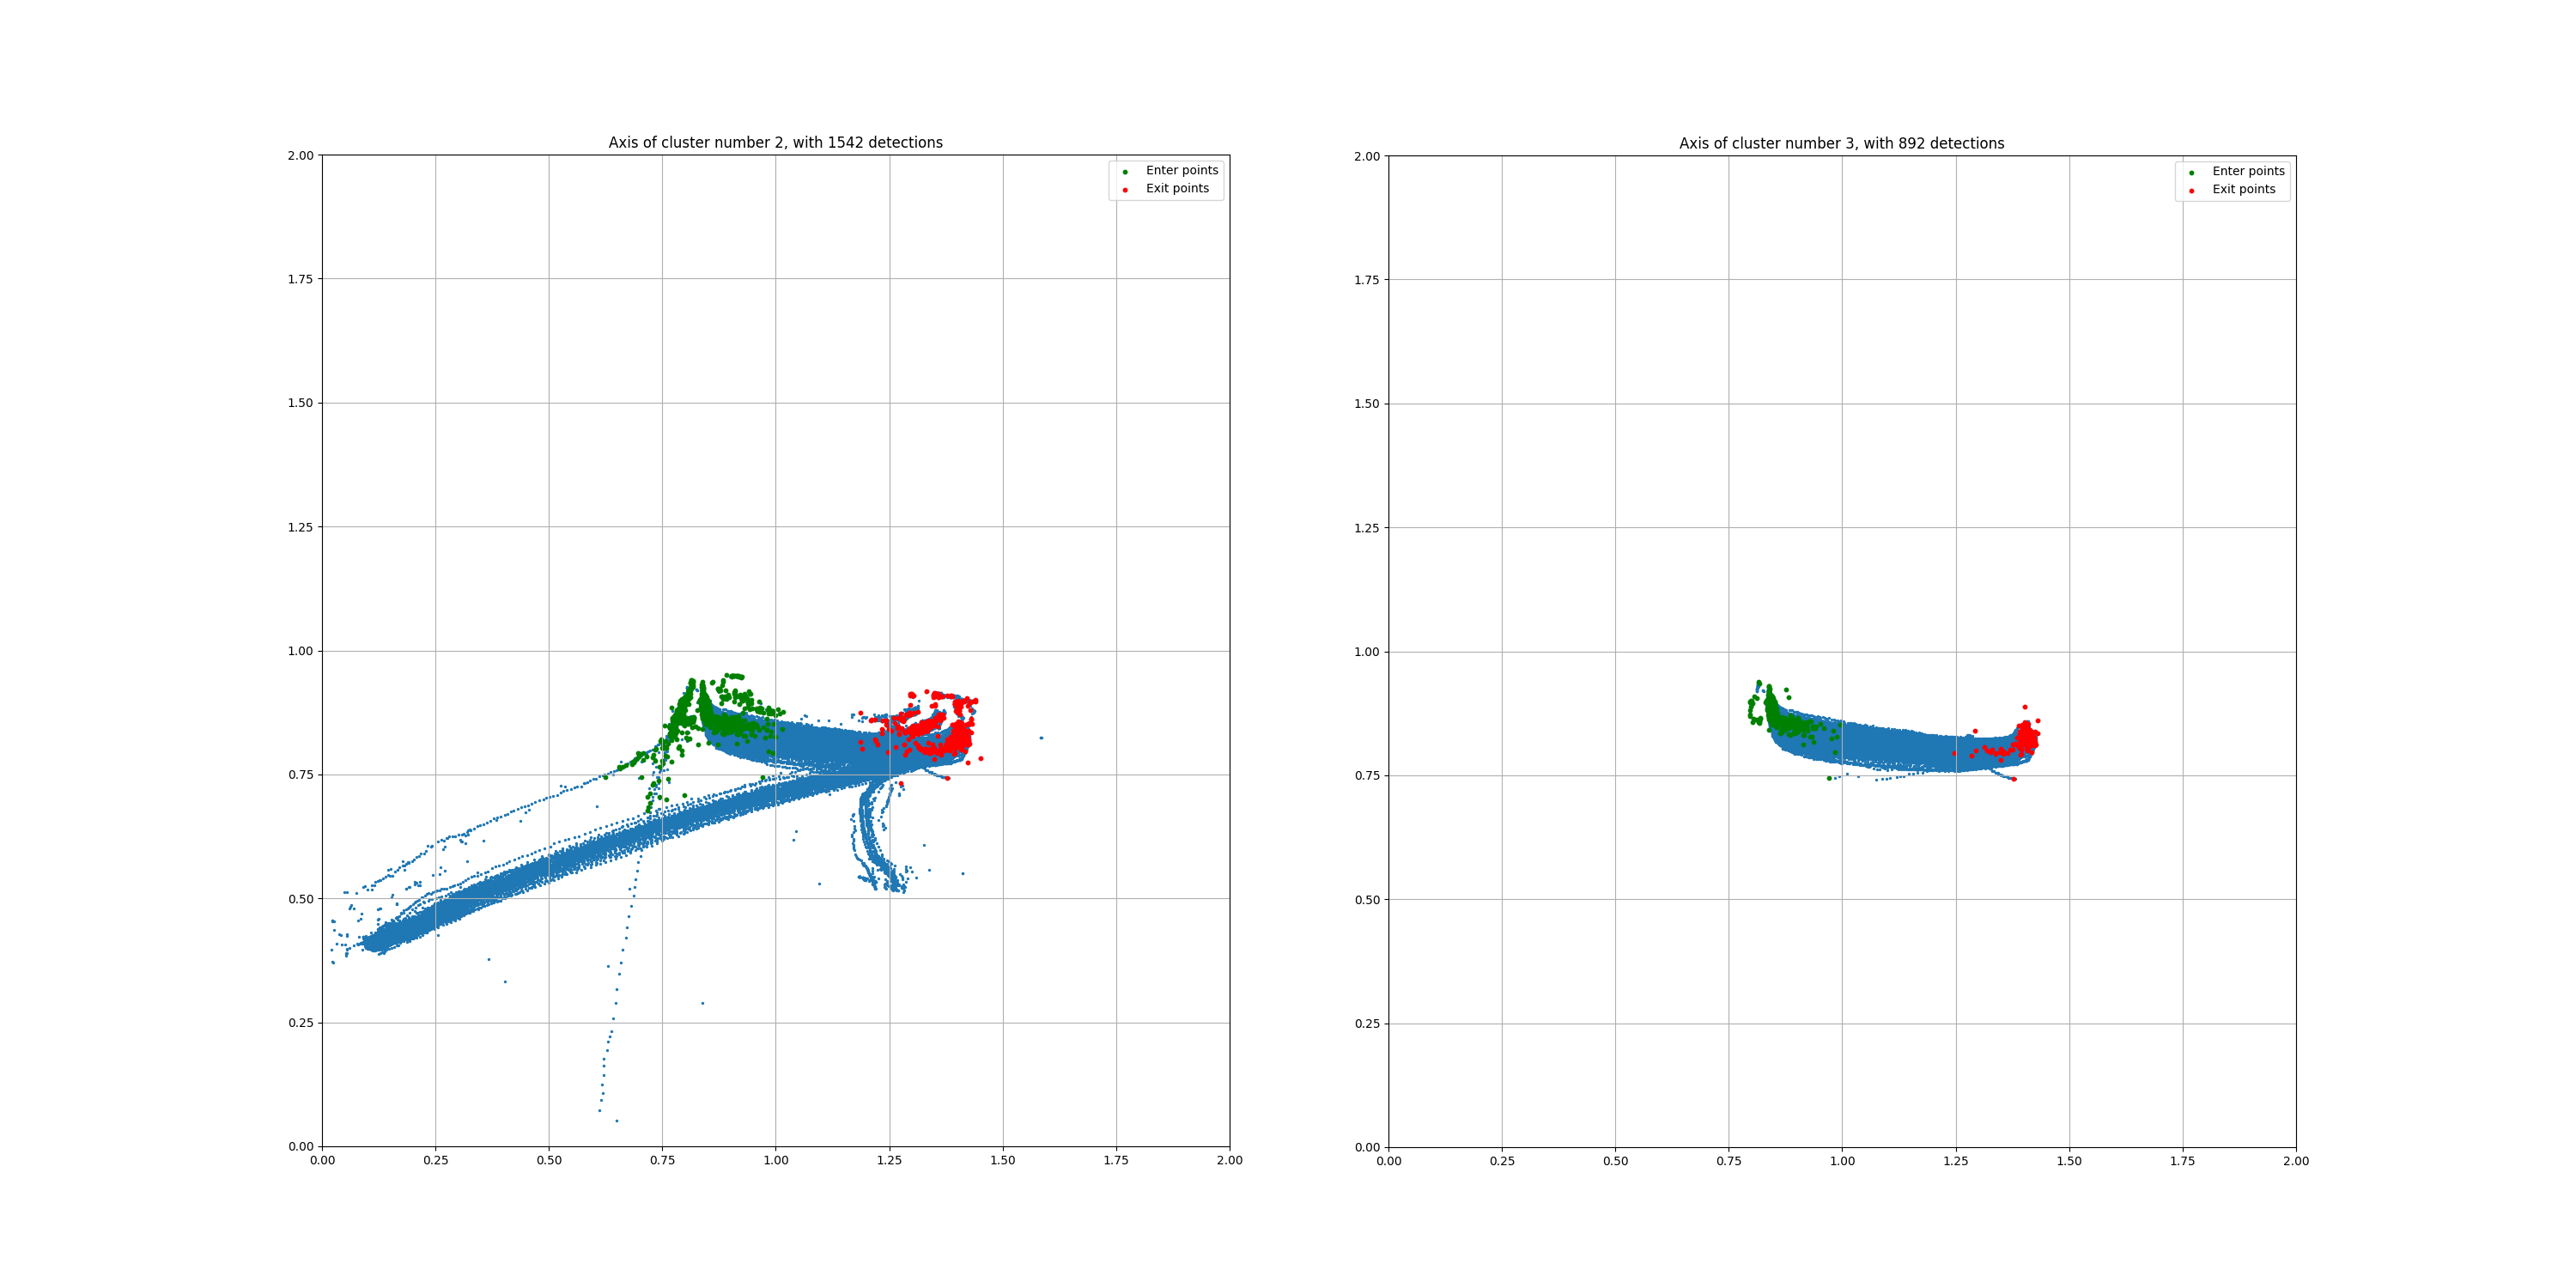
\includegraphics[width=0.8\columnwidth]{clustering/n_cluster_2_before_after.png}
 \caption{Klaszterezés szűrő}
 \label{fig: Klaszterezés szűrő}   
\end{figure}
\begin{figure}[H]
 \centering
 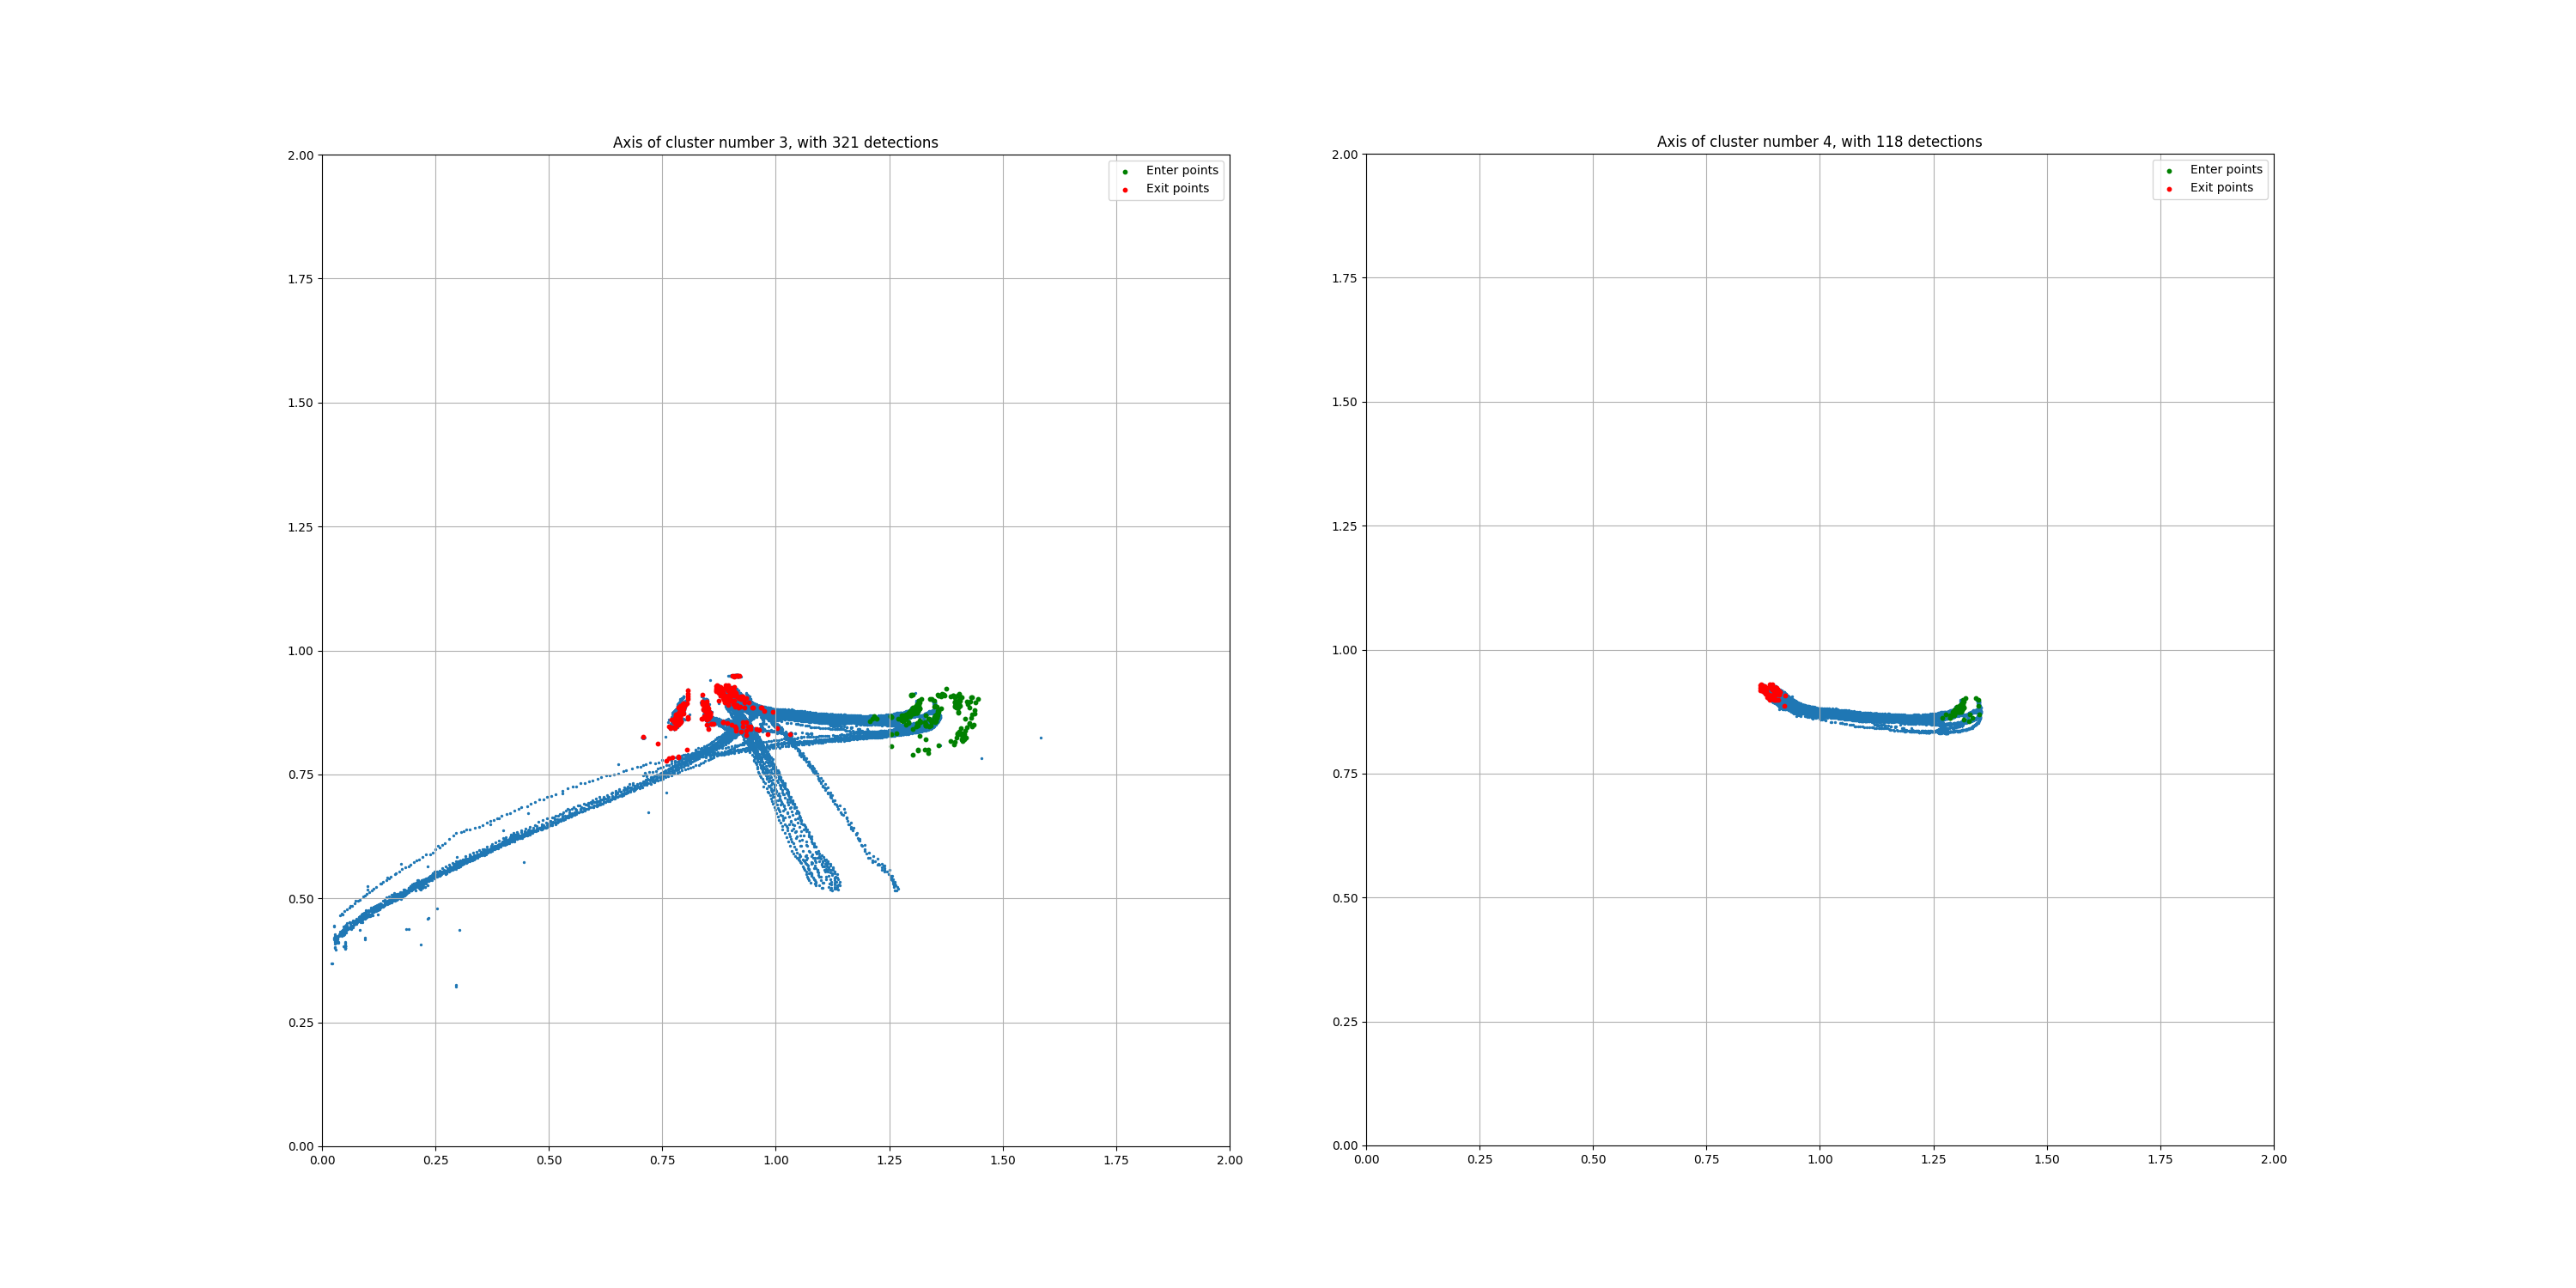
\includegraphics[width=0.8\columnwidth]{clustering/n_cluster_3_before_after.png}
 \centering
 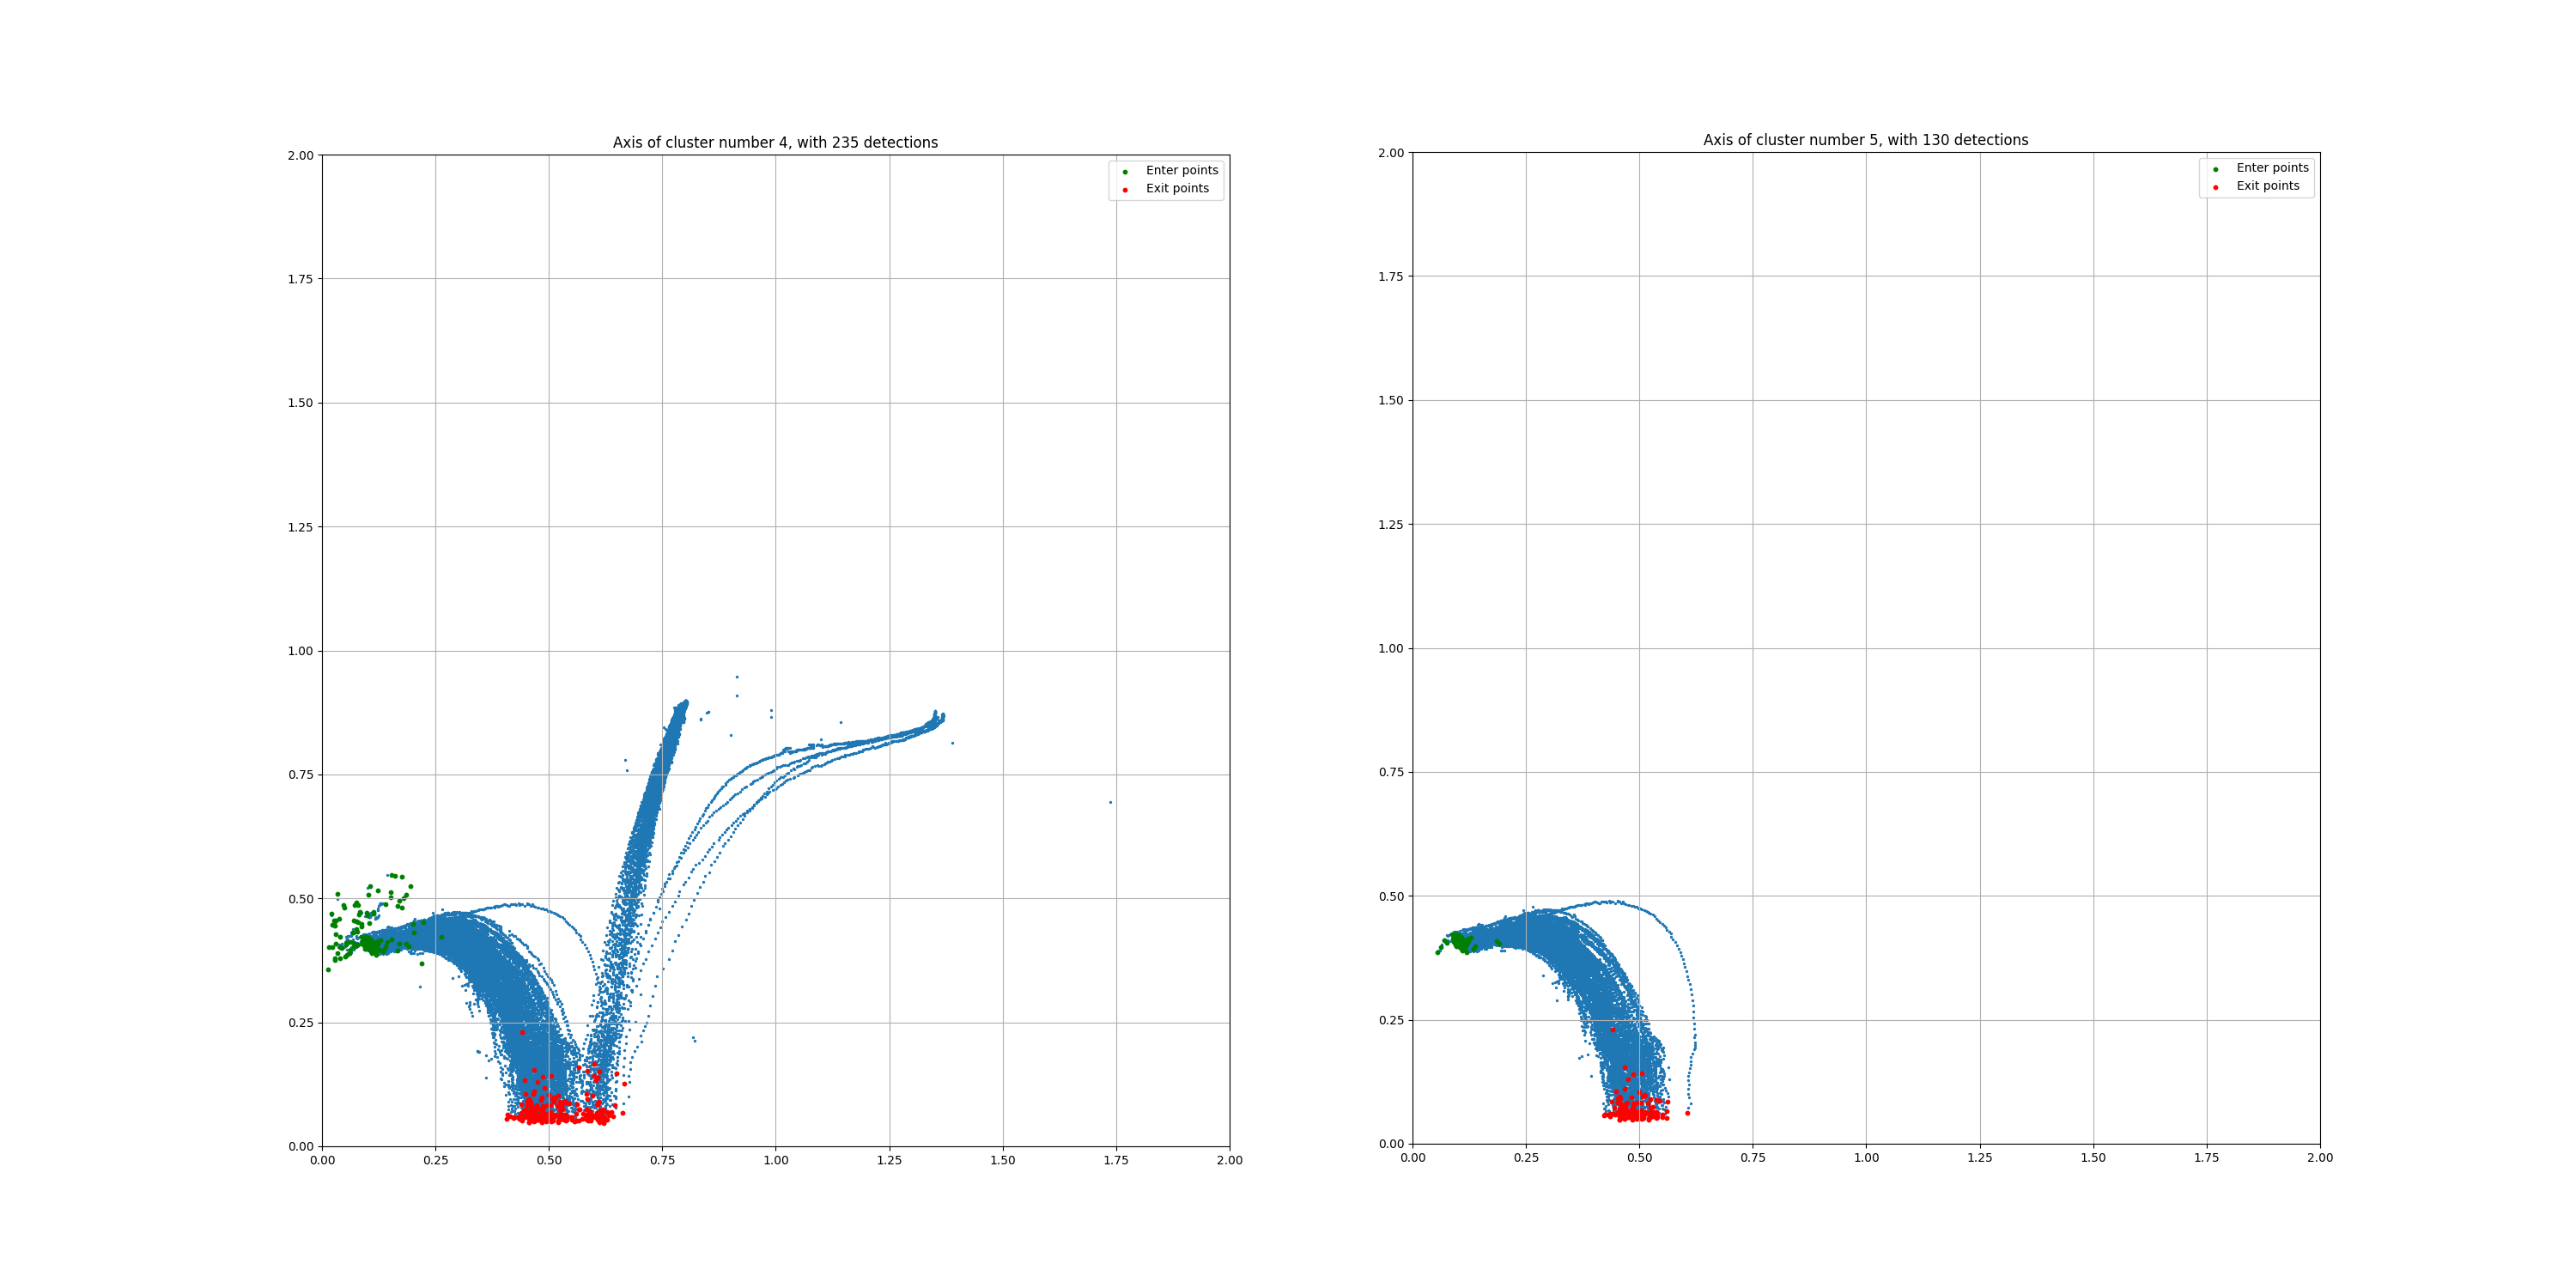
\includegraphics[width=0.8\columnwidth]{clustering/n_cluster_4_before_after.png}
 \centering
 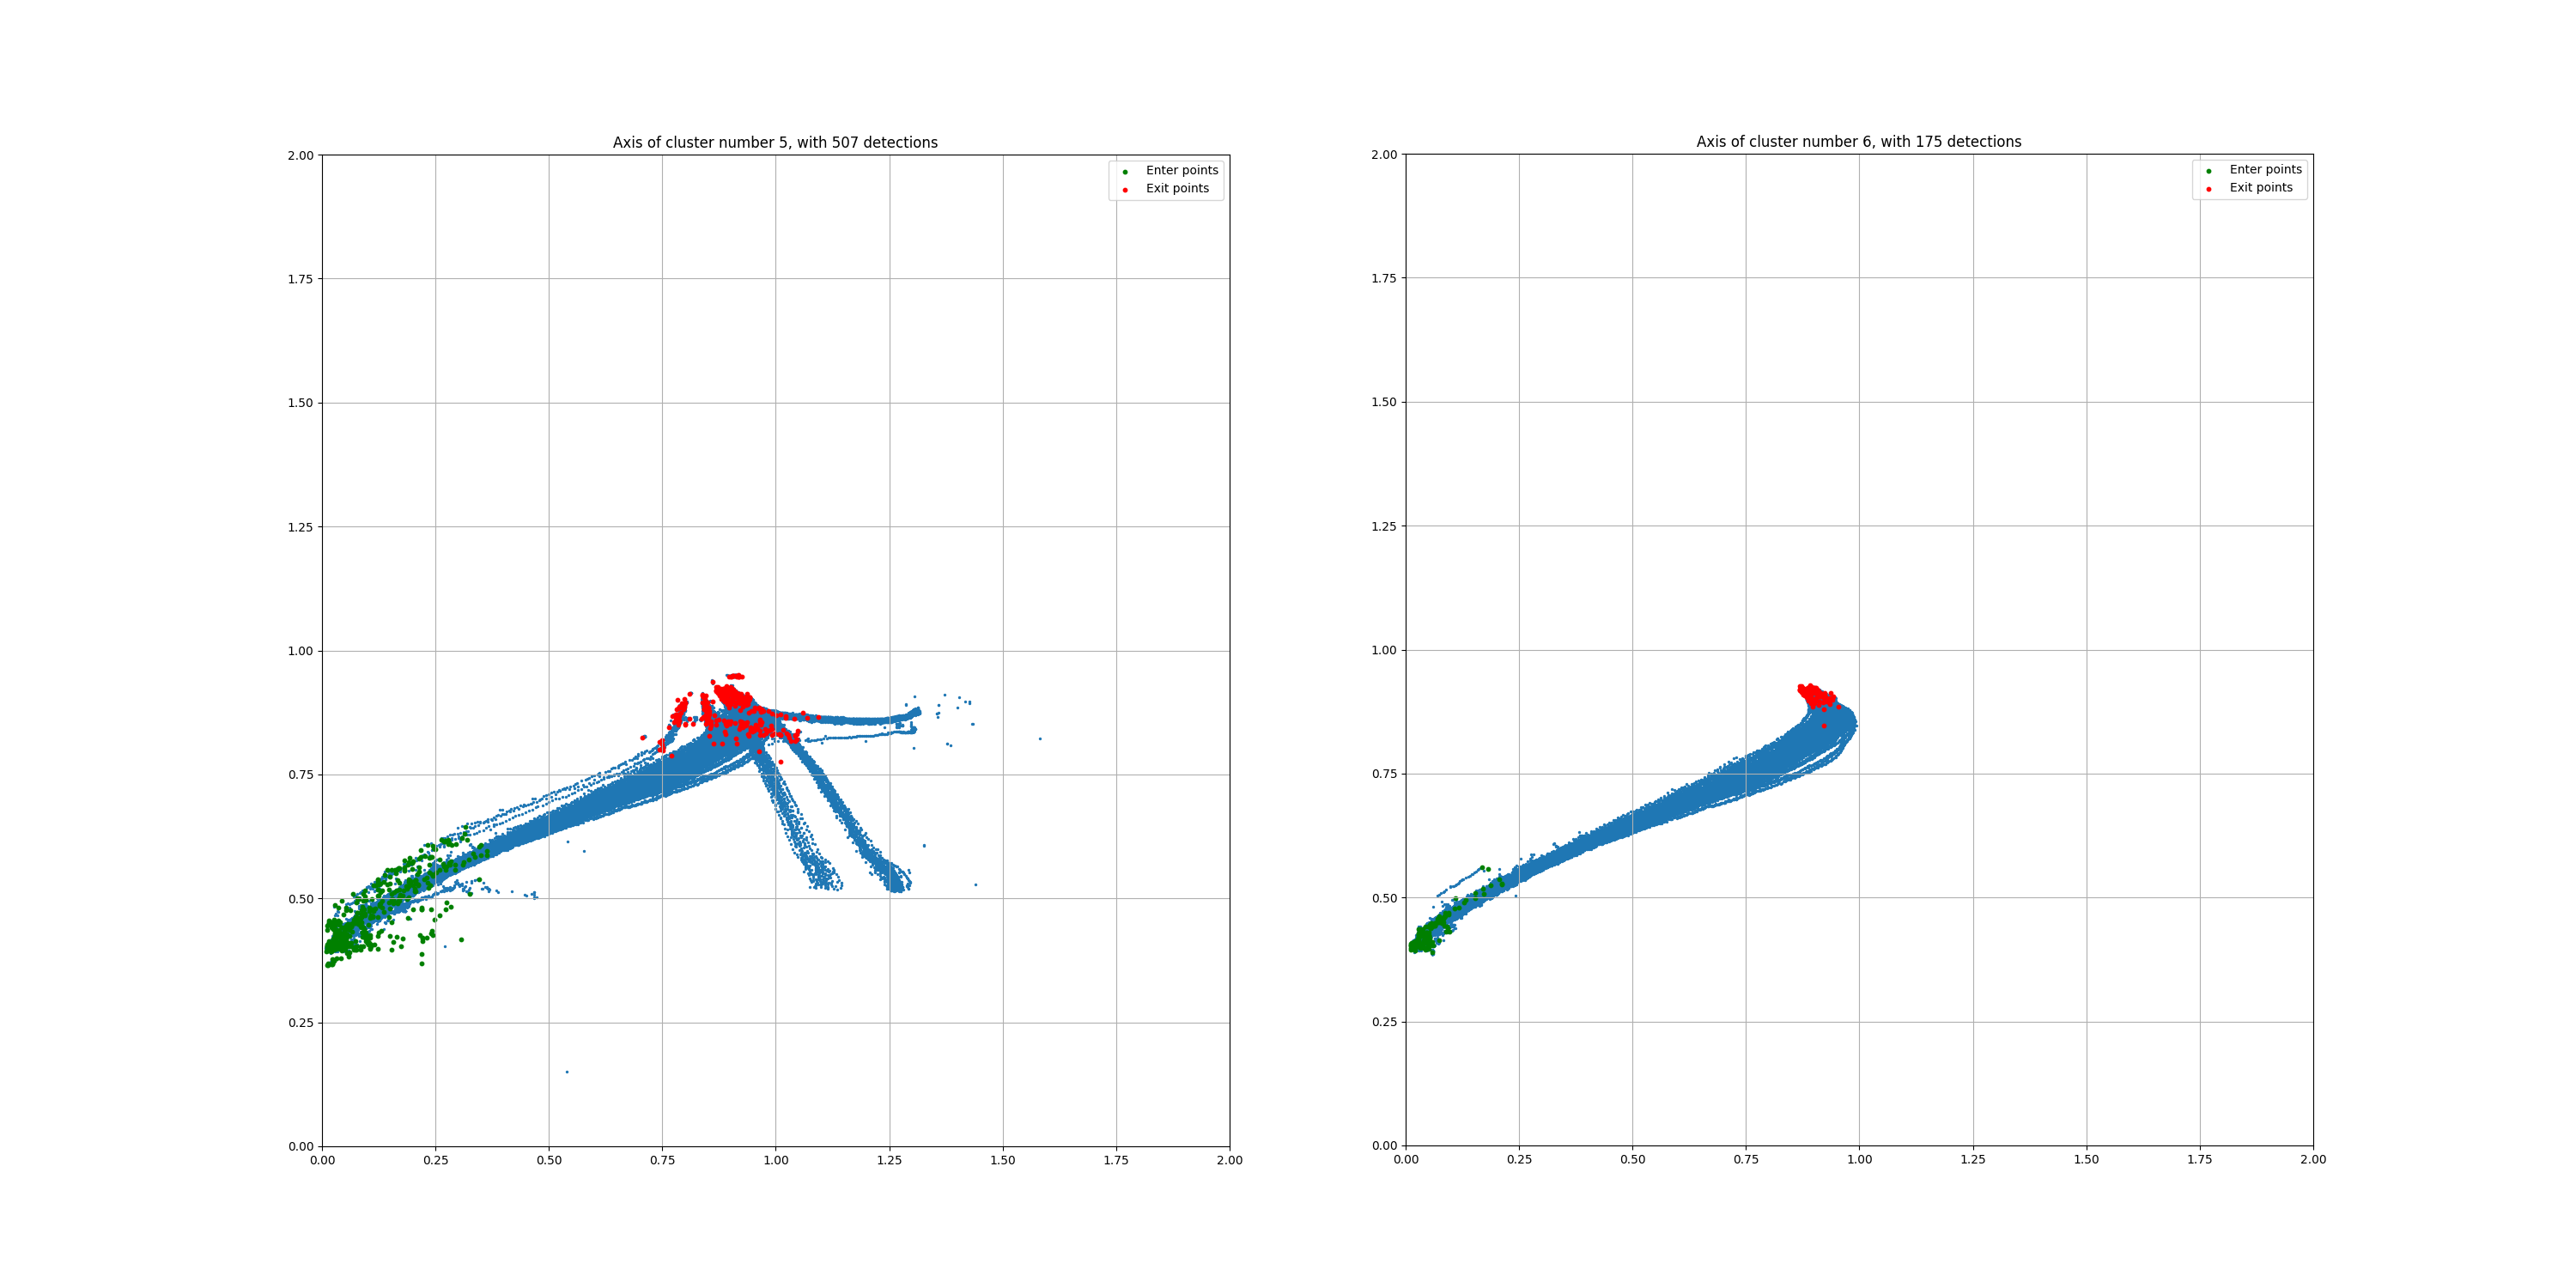
\includegraphics[width=0.8\columnwidth]{clustering/n_cluster_5_before_after.png}
 \caption{Klaszterezés szűrő}
 \label{fig: Klaszterezés szűrő2}   
\end{figure}
\begin{figure}[H]
 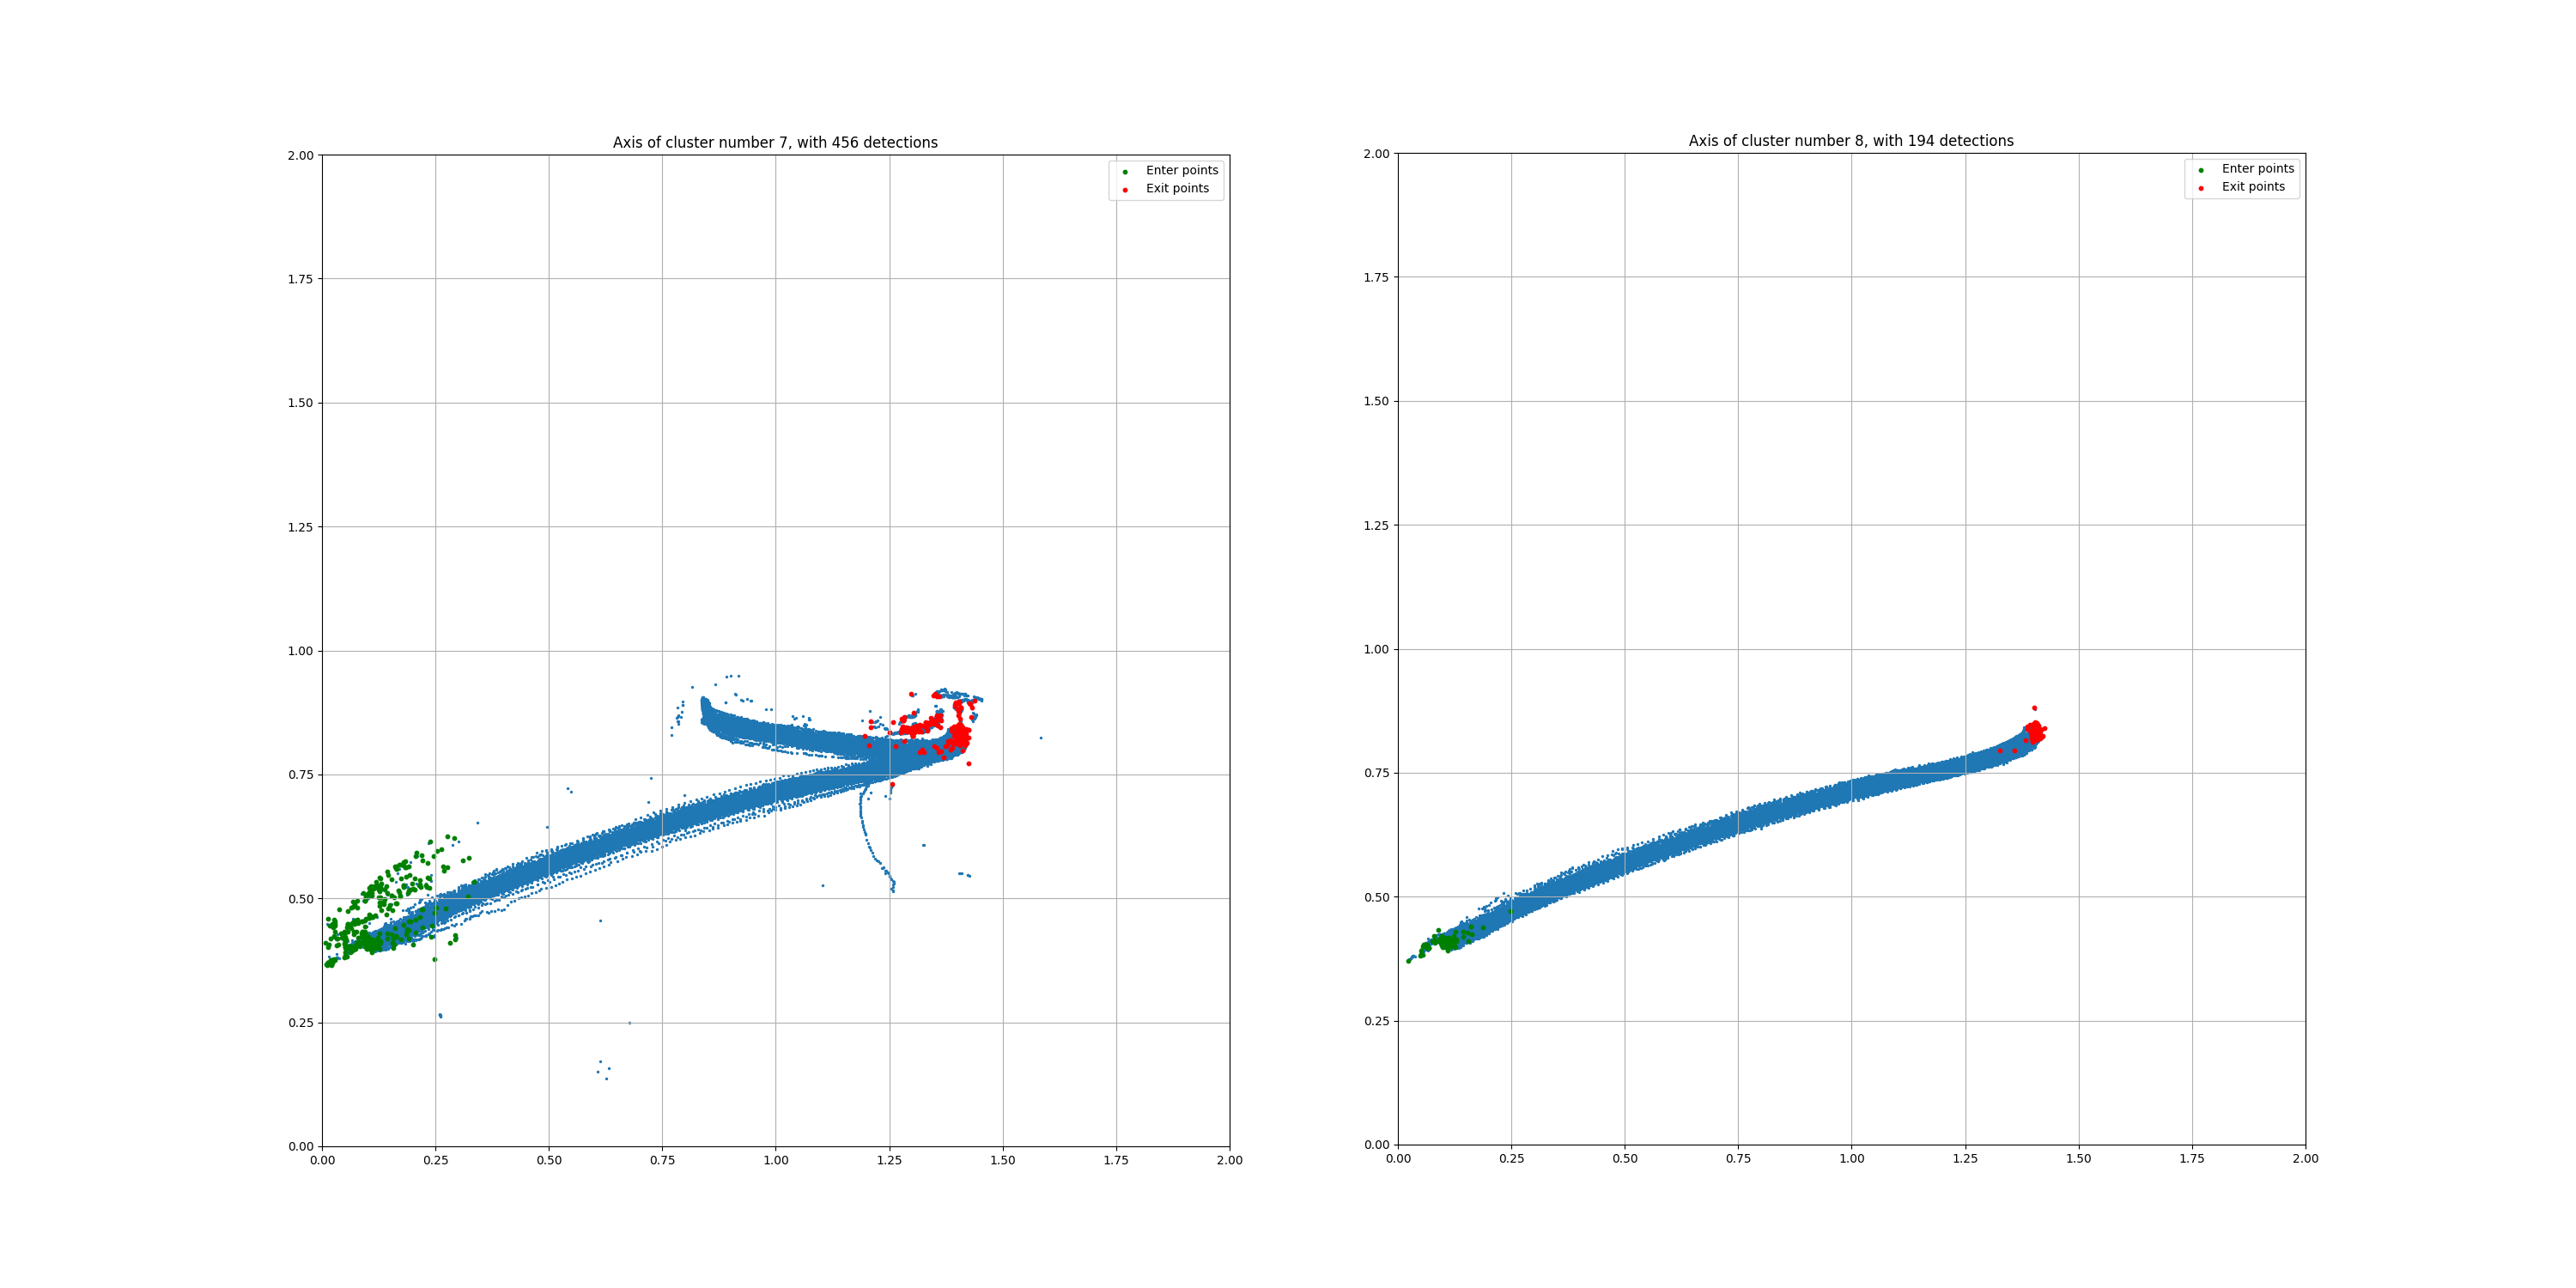
\includegraphics[width=1\columnwidth]{clustering/n_cluster_7_before_after.png}
 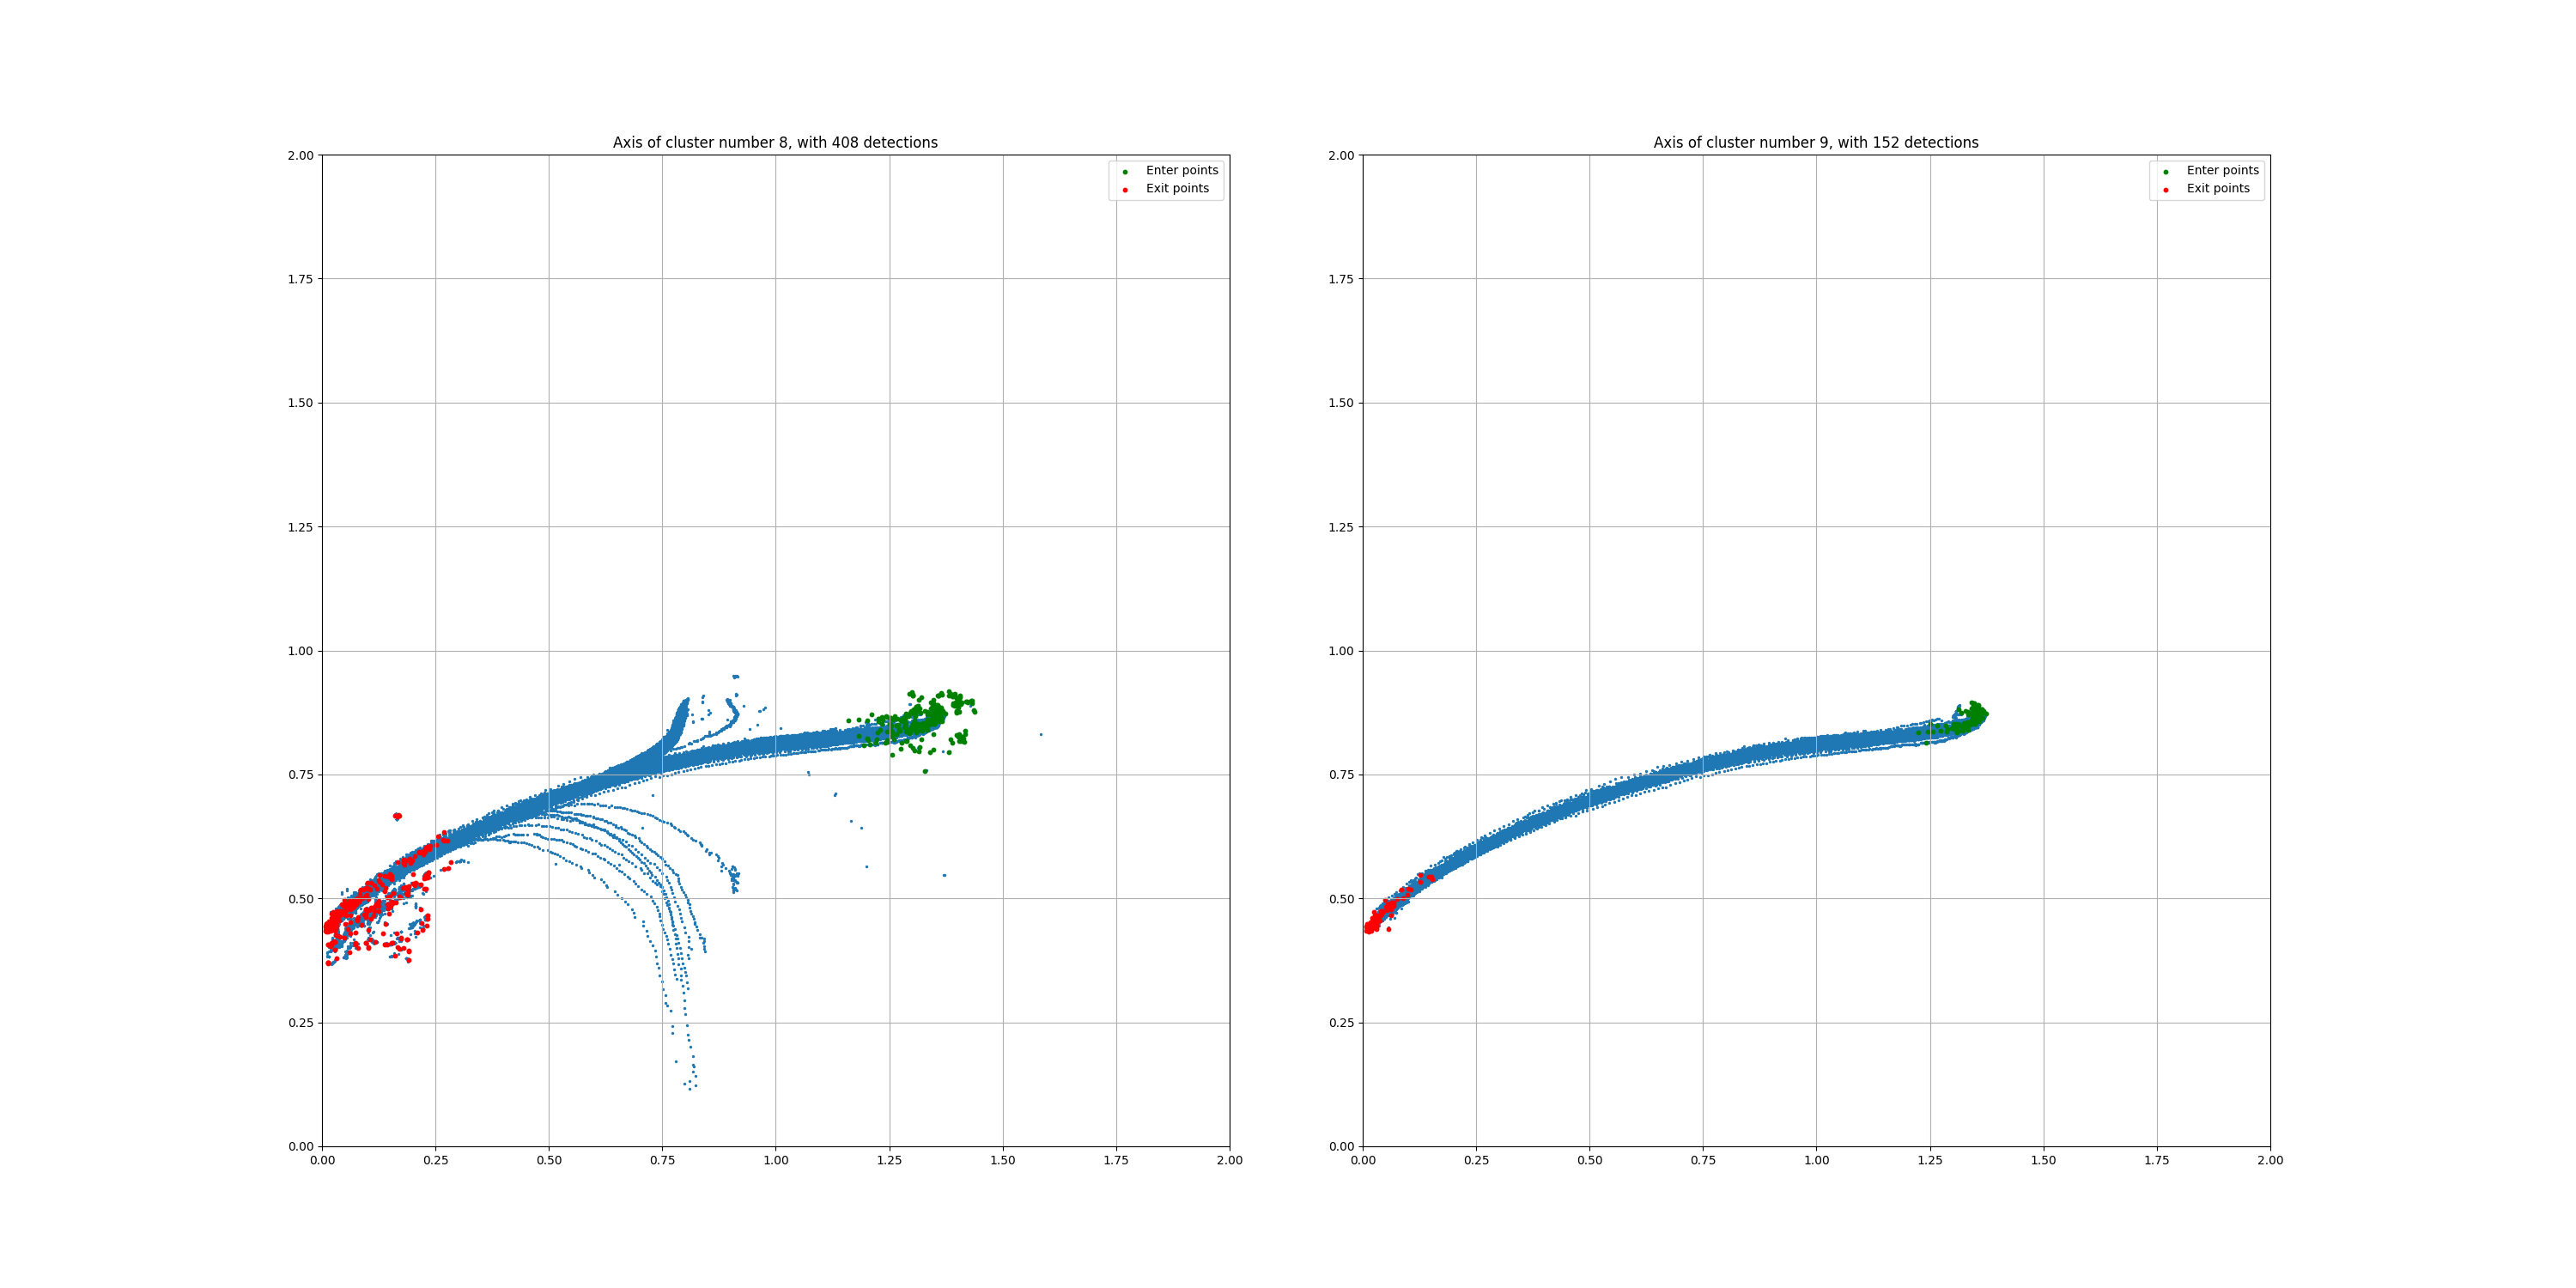
\includegraphics[width=1\columnwidth]{clustering/n_cluster_8_before_after.png}
 \caption{Klaszterezés szűrő}
 \label{fig: Klaszterezés szűrő3}   
\end{figure}

\subsection{Feature vektorok}
Klaszterezéshez 4 és 6 dimenziós feature vektorokat használ-tunk. A 6 dimenziós vektorokat a DeepSORT hibájának a kiszűrésére hoztuk létre, felépítésük a következő [belépő x,y középső x,y kilépő x,y], de a kifejlesztett szűrő hatékonyab-bnak bizonyult, és a kevesebb dimenzió is előnyt jelent, ezért maradtunk a 4 dimenziós feature vektor mellett, aminek a felépítése: [belépő x,y kilépő x,y].
\subsection{Klaszterezési algoritmusok}
Klaszterezéshez több fajta algoritmust teszteltünk. A legjobb eredményeket az OPTICS (Ordering Points To Identify the Clustering Structure) \cite{10.1145/304181.304187} algoritmus adta. 
Aminek az eredményei a fenti képeken látható (lásd. \ref{fig: Bad clusters}). A képen bal oldalon láthatók rendre a KMeans, DBSCAN és BIRCH által rendezett klaszterek, a jobb oldalon pedig az OPTICS által rendezett klaszterek. Az utolsó sorban a BIRCH eredménye látható, ahol két klasztert egybevont, amit az OPTICS meg tudott különböztetni.
OPTICS-on kívül teszteltük a KMeans, DBSCAN és BIRCH algoritmusokat. 
\paragraph{KMeans} A KMeans klaszterezés egy unsupervised machine learning algoritmus, amely célja az adatok csoportosítása oly módon, hogy azonos klaszterbe tartozó adatok közötti távolság minimális legyen, míg az eltérő klaszterek közötti távolság maximális.
Az algoritmus működése a következő lépésekből áll:
\begin{enumerate}
    \item Centroidok inicializálása: Az algoritmus véletlenszerűen inicializál k centroidot a dataseten, ahol k a klaszterek száma.
    \item Adatok csoportosítása: Az algoritmus minden adatponthoz hozzárendeli a legközelebbi centroidot, és azonos klaszterbe helyezi azokat az adatpontokat, amelyeknek a centroidja megegyezik.
    \item Centroidok újraszámolása: Az algoritmus újraszámolja a centroidok pozícióit az adatok csoportosítása után, hogy azok a klaszterben található adatpontok átlagértékének megfelelően helyezkedjenek el.
    \item Lépések ismétlése: Az algoritmus addig ismételgeti a 2. és 3. lépéseket, amíg az adatpontok klaszterezése konvergens állapotba nem jut, azaz az adatpontok csoportosítása már nem változik, vagy az algoritmus előre meghatározott maximális iterációs számhoz ér.
    \item Klaszterek értékelése: Az algoritmus kiértékeli a klaszterek minőségét, például a csoportokban lévő adatpontok közötti távolságot, és eldönti, hogy a csoportokat újra kell-e szervezni.
\end{enumerate}
A KMeans klaszterezés előnye, hogy egyszerű és gyors algoritmus, amely hatékonyan használható az adatok csoportosítására. A klaszterek számát könnyen meg lehet adni, és az algoritmus gyorsan konvergál. Azonban az algoritmus érzékeny az inicializálási folyamatokra, és gyakran találhatók olyan csoportok, amelyek nem teljesen homogének.
Emellett KMeans $n\_clusters$ - klaszterek száma - paraméterét előre kell definiálni, aminek meghatározására próbálkoztunk különböző metrikákat felhasználni, hogy automatizálható legyen
a klaszterezési lépés. Ezek a metrikák a Silhouette Coefficient \cite{ROUSSEEUW198753}, Calinski-Harabasz Index \cite{article} és Davies-Bouldin Index \cite{4766909}.
Elbow diagramok segítségével próbáltuk eldönteni, hogy milyen értéket érdemes adni az \begin{math}n\_clusters\end{math} paraméternek lásd \ref{fig: Elbow diagramok}.
A mérőszámok konzisztensen alacsony értéket adtak, egy négyágú kereszteződésnél, ahol jóval több klaszterbe sorolhatók a trajektóriák. A KMeans használatát
ezért elvetettük.

\begin{figure}
    \centering
    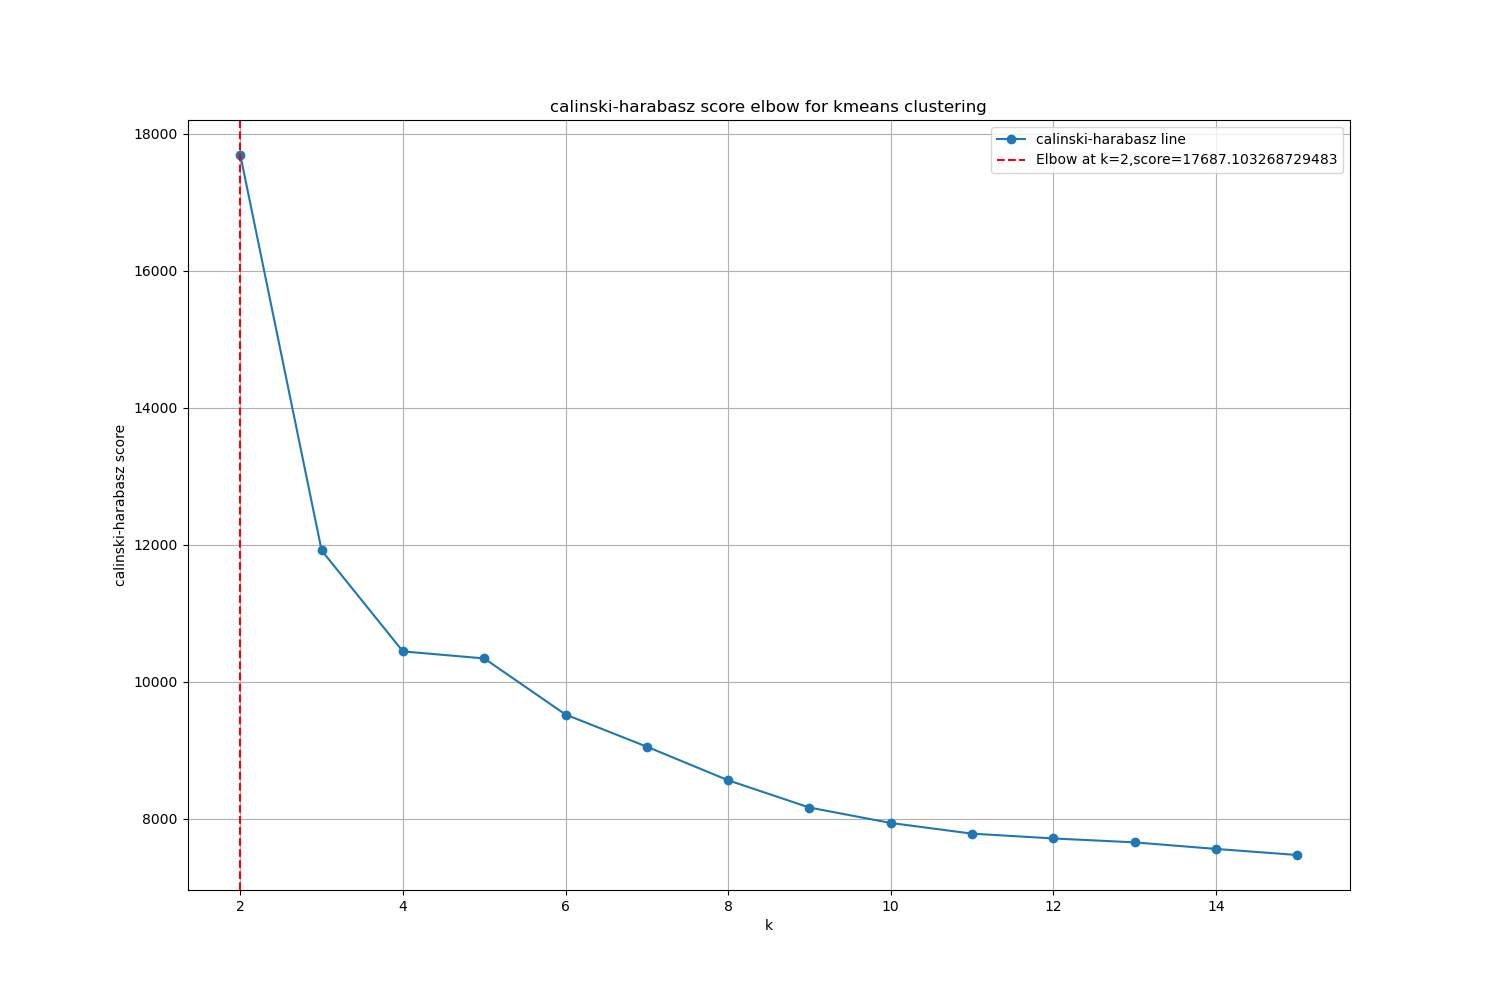
\includegraphics[width=0.7\columnwidth]{elbow/elbow_on_kmeans_2-16_metric_calinski-harabasz_thresh_0.5.png}
    \centering
    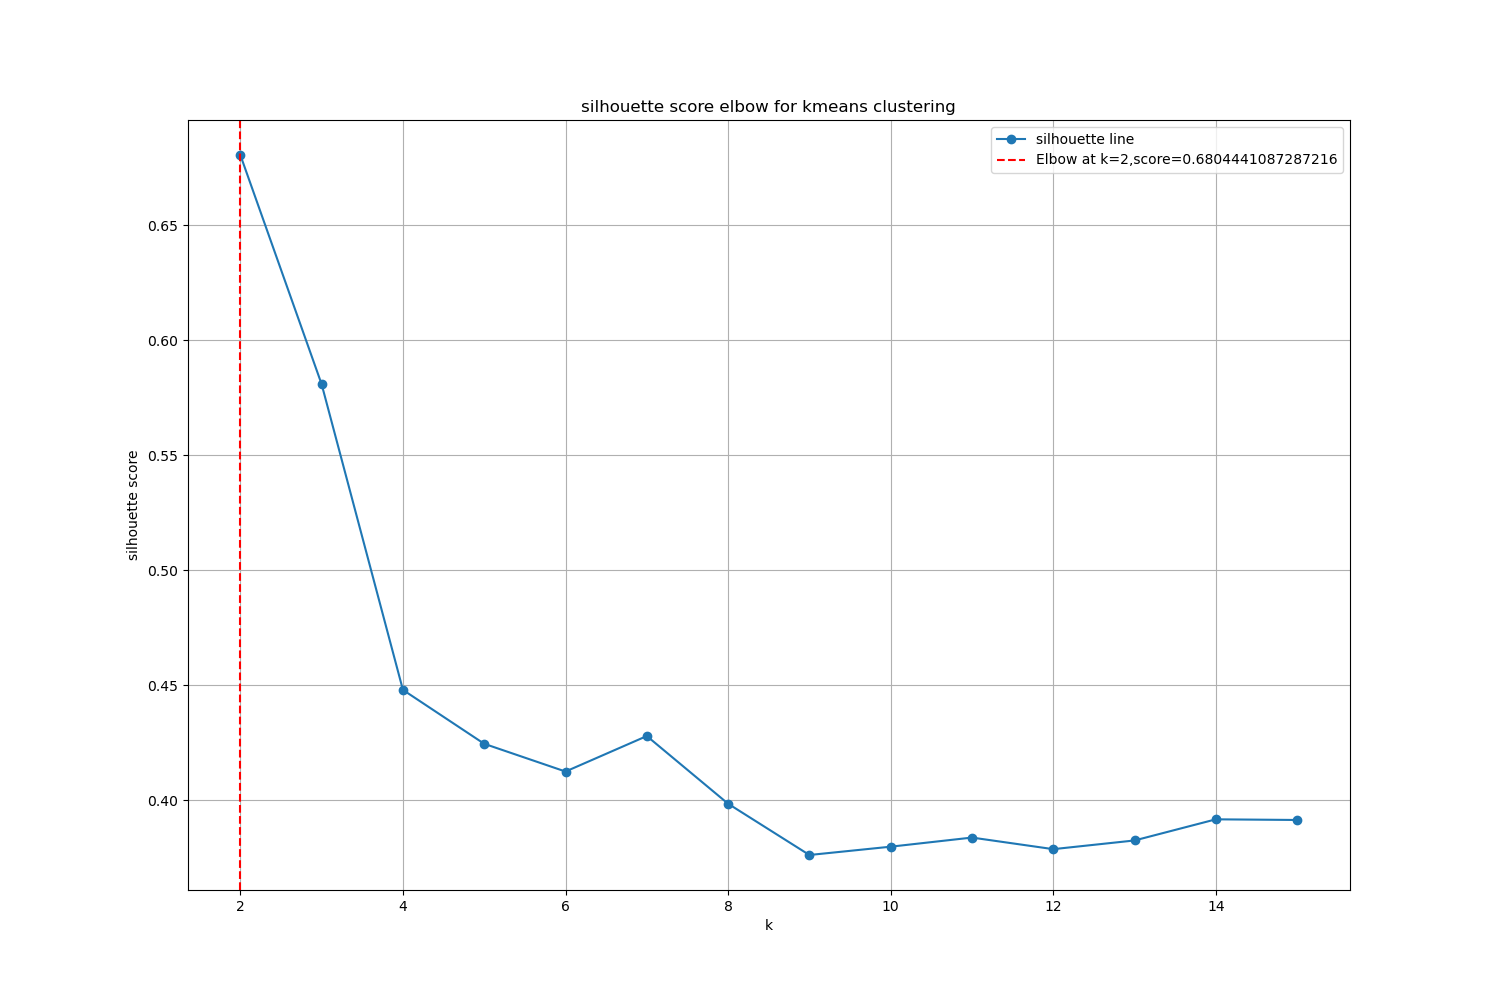
\includegraphics[width=0.7\columnwidth]{elbow/elbow_on_kmeans_2-16_metric_silhouette_thresh_0.5.png}
    \centering
    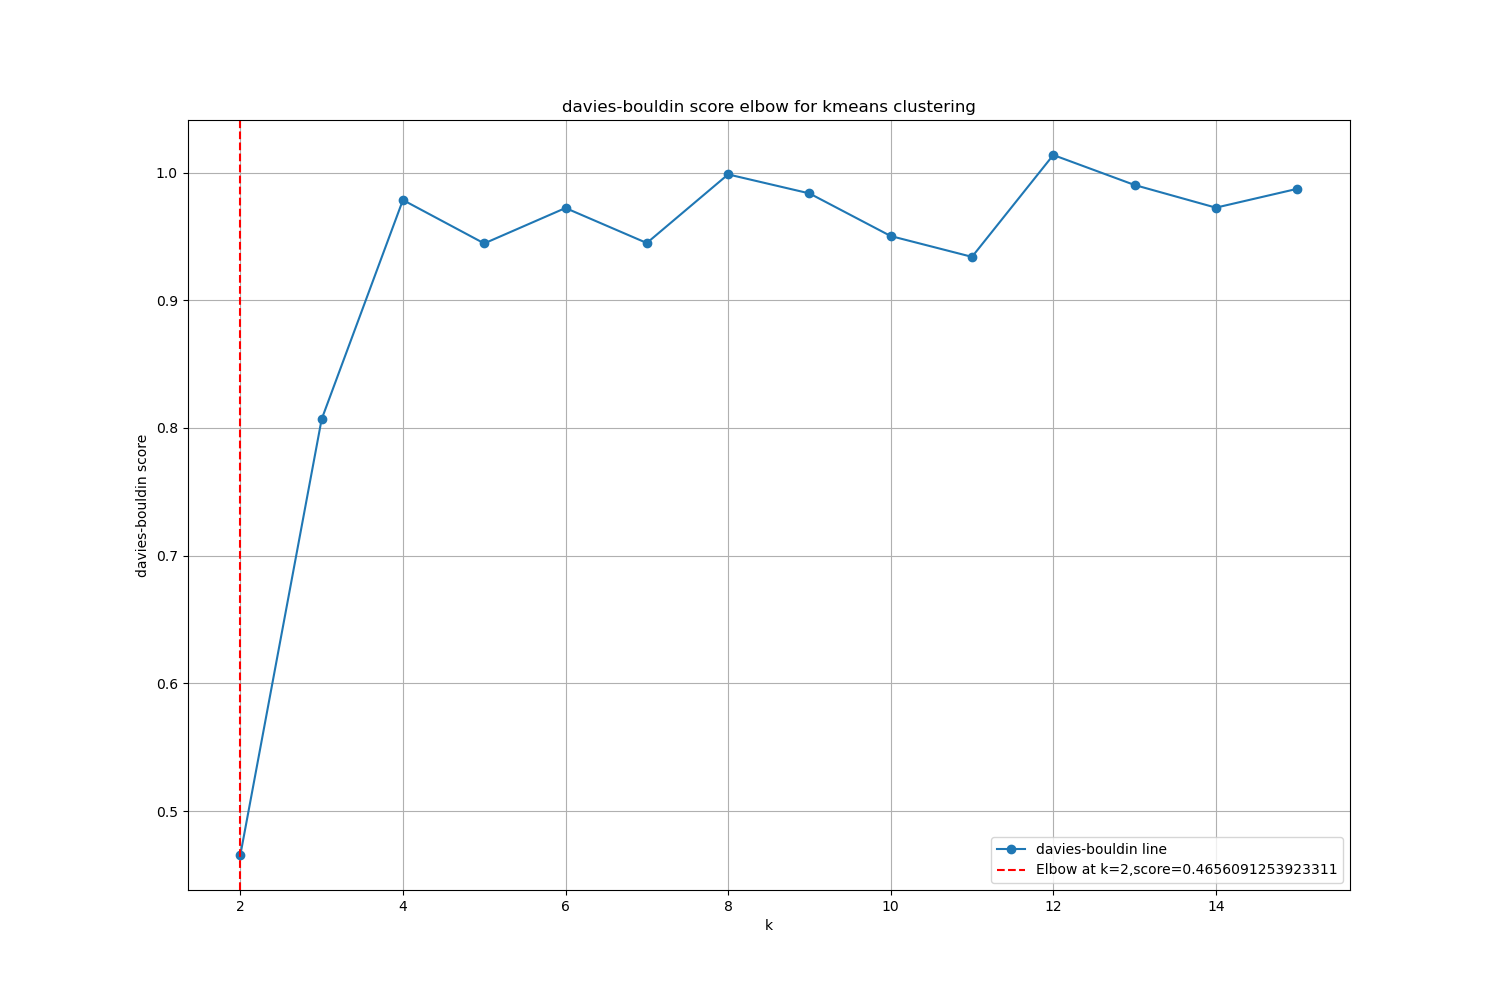
\includegraphics[width=0.68\columnwidth]{elbow/elbow_on_kmeans_2-16_metric_davies-bouldin_thresh_0.5.png}
    
    \caption{Elbow diagramok}
    \label{fig: Elbow diagramok}
\end{figure}

\begin{figure}
    \centering
    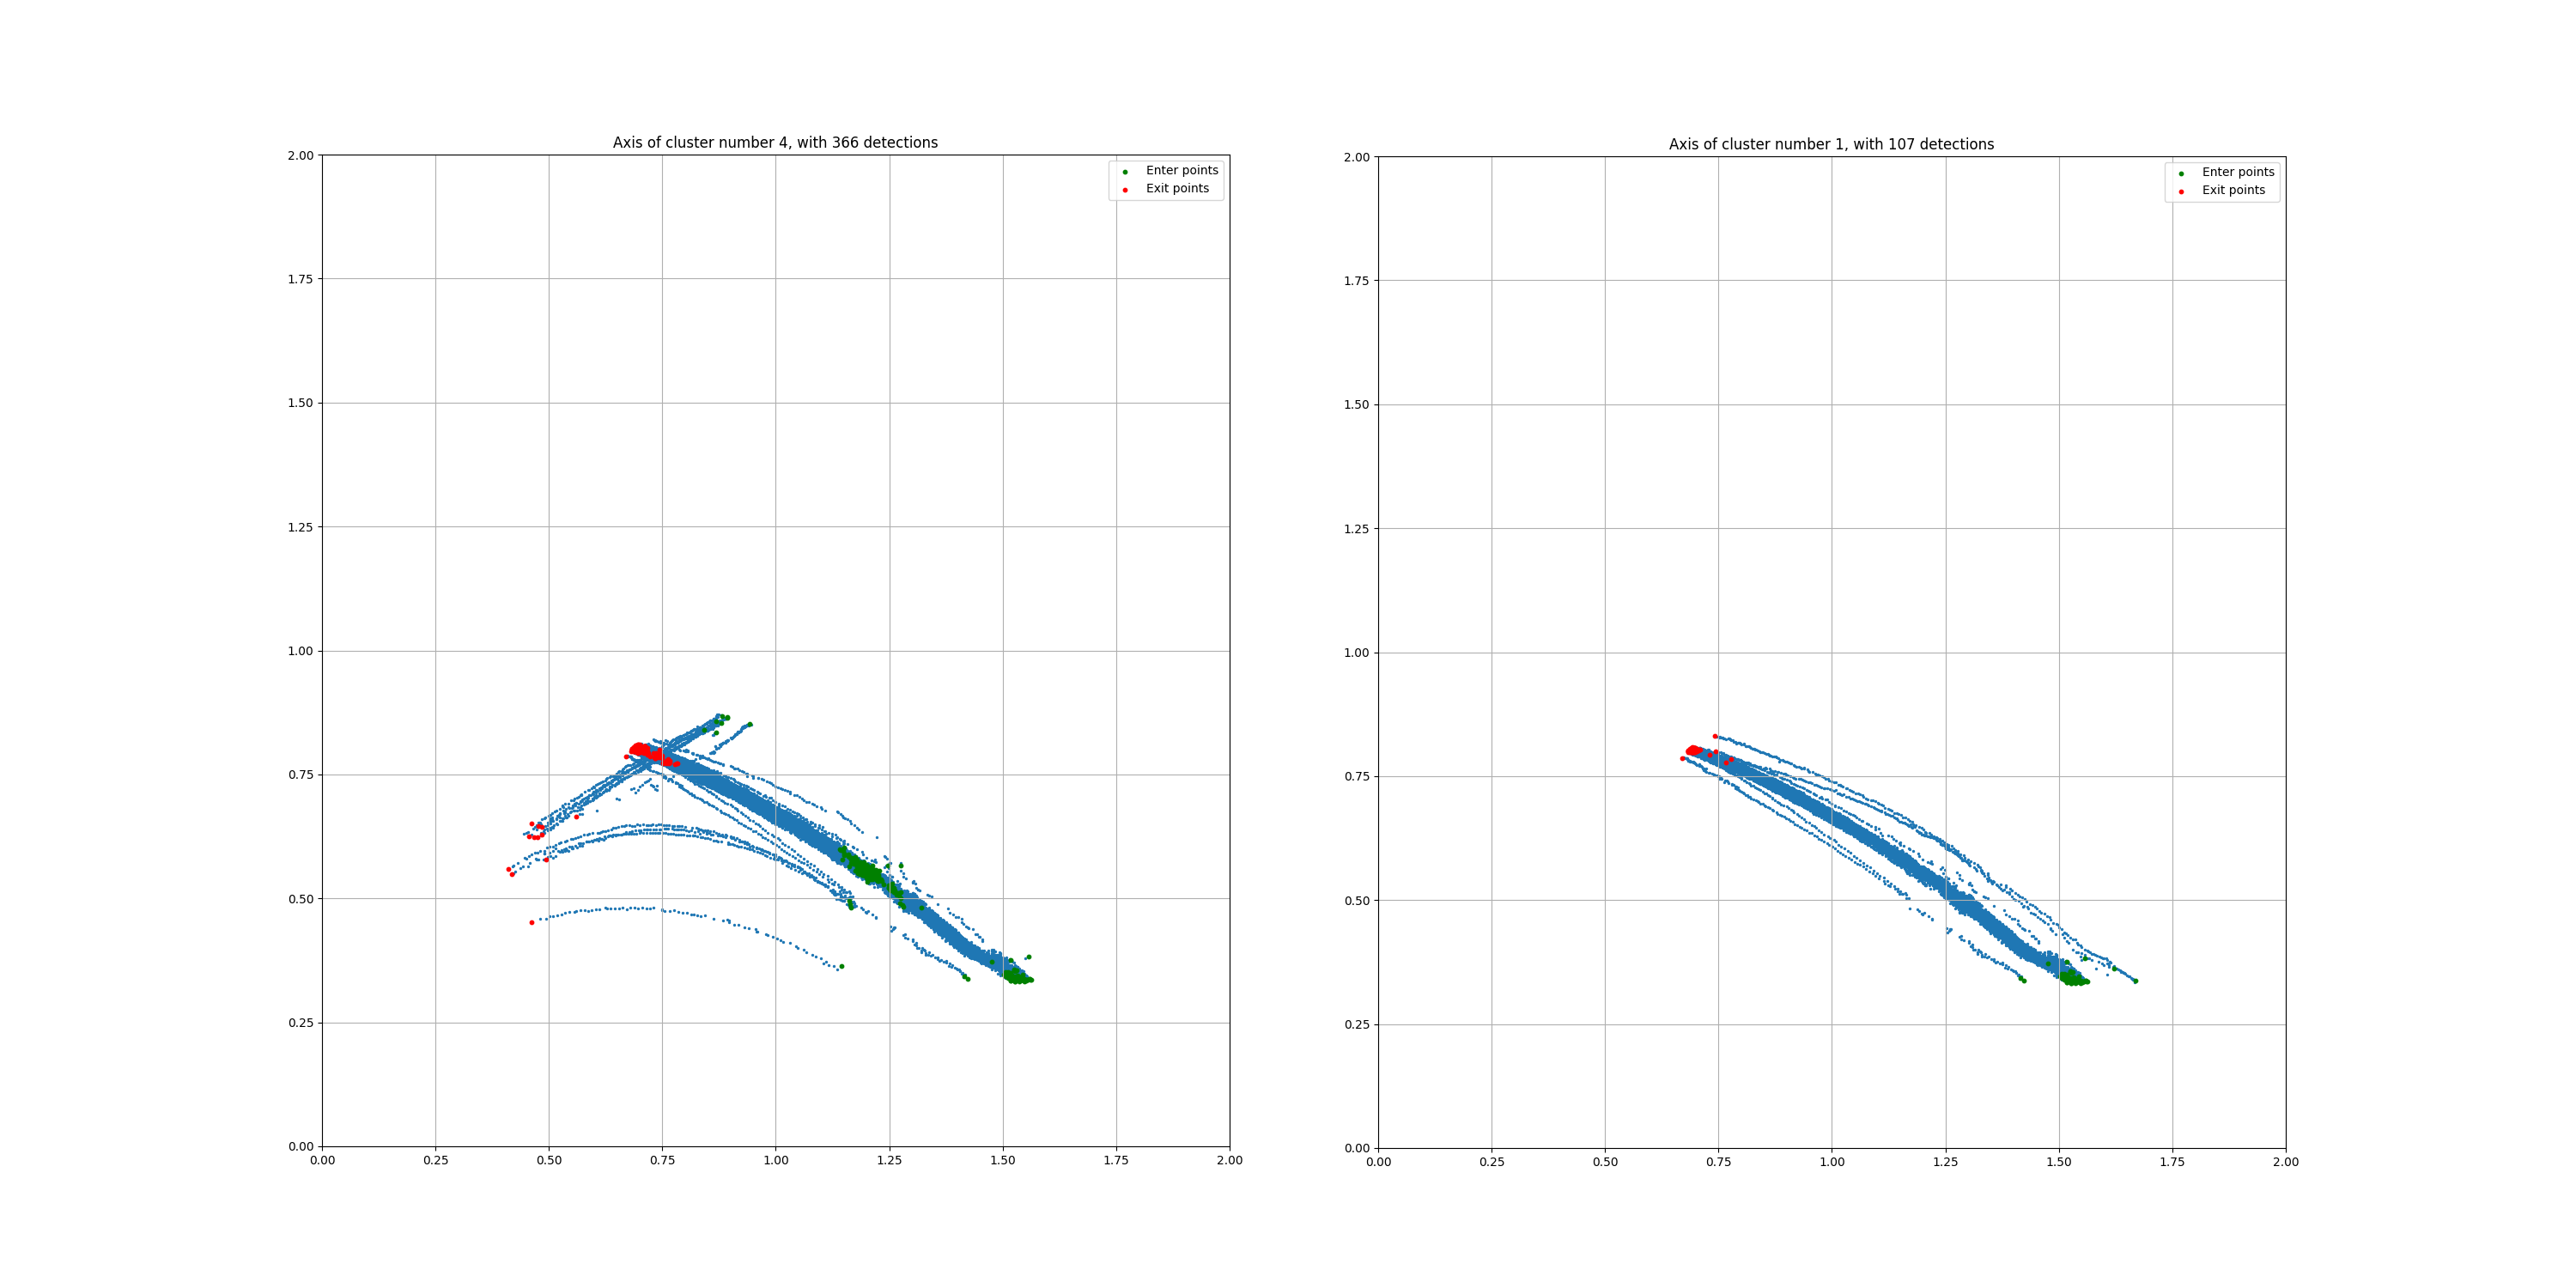
\includegraphics[width=0.65\columnwidth]{bad_clustering/example_kmeans_vs_optics.png}
    \centering
    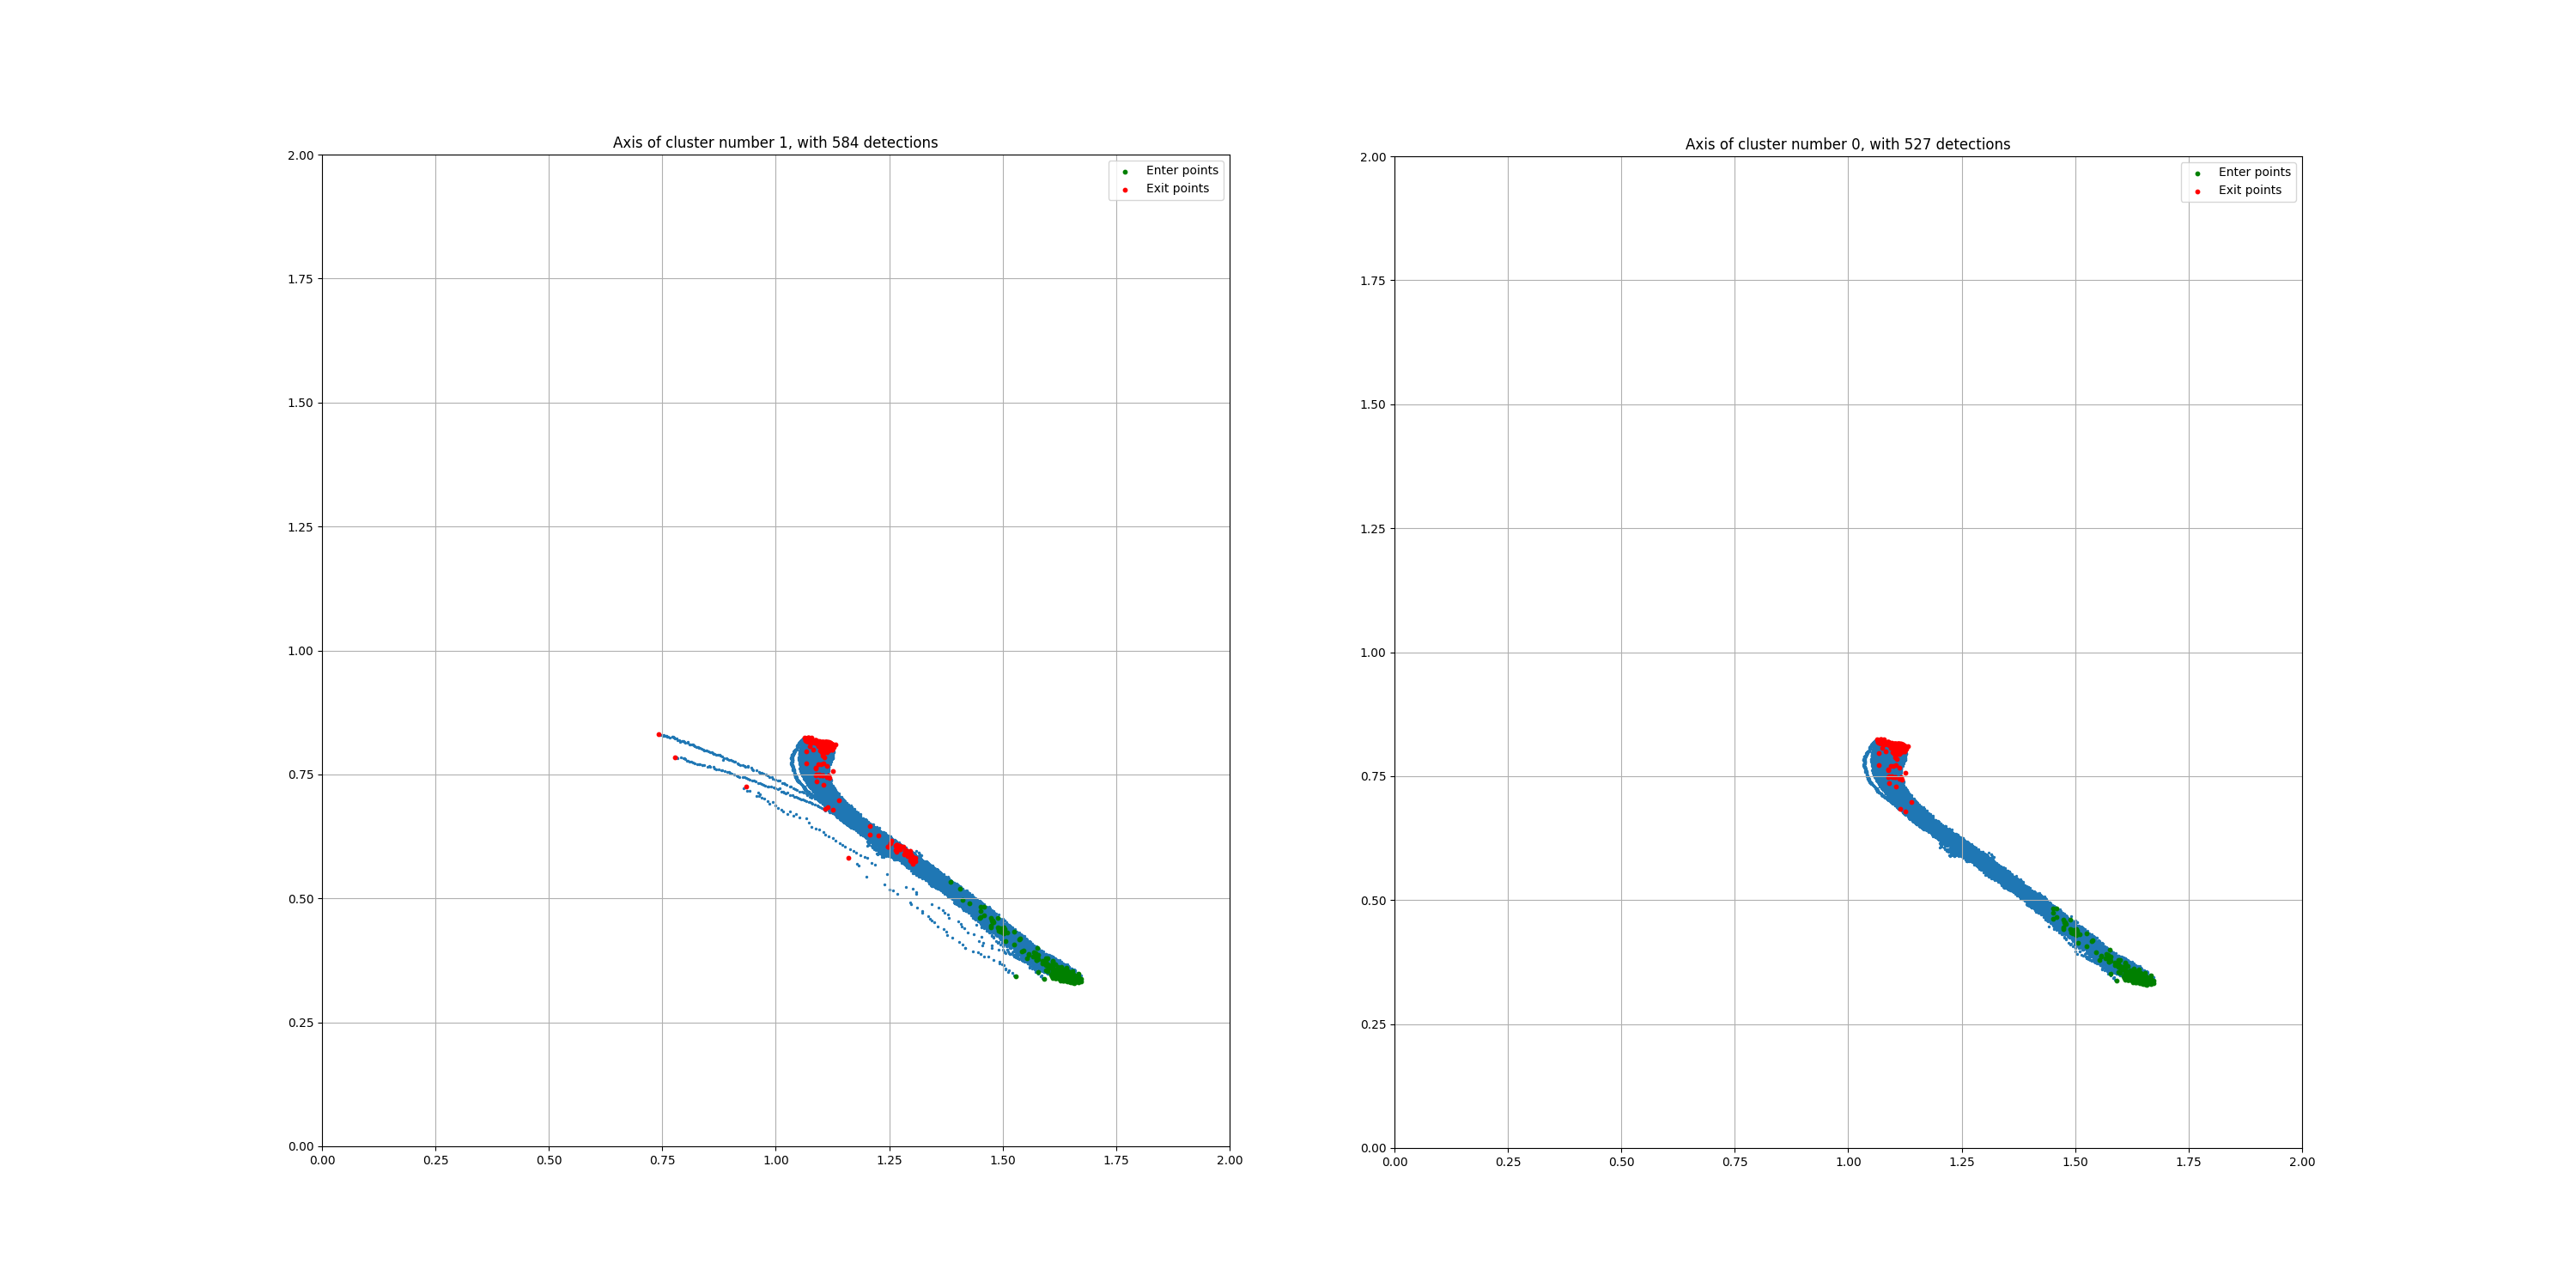
\includegraphics[width=0.65\columnwidth]{bad_clustering/example_birch_vs_optics.png}
    \centering
    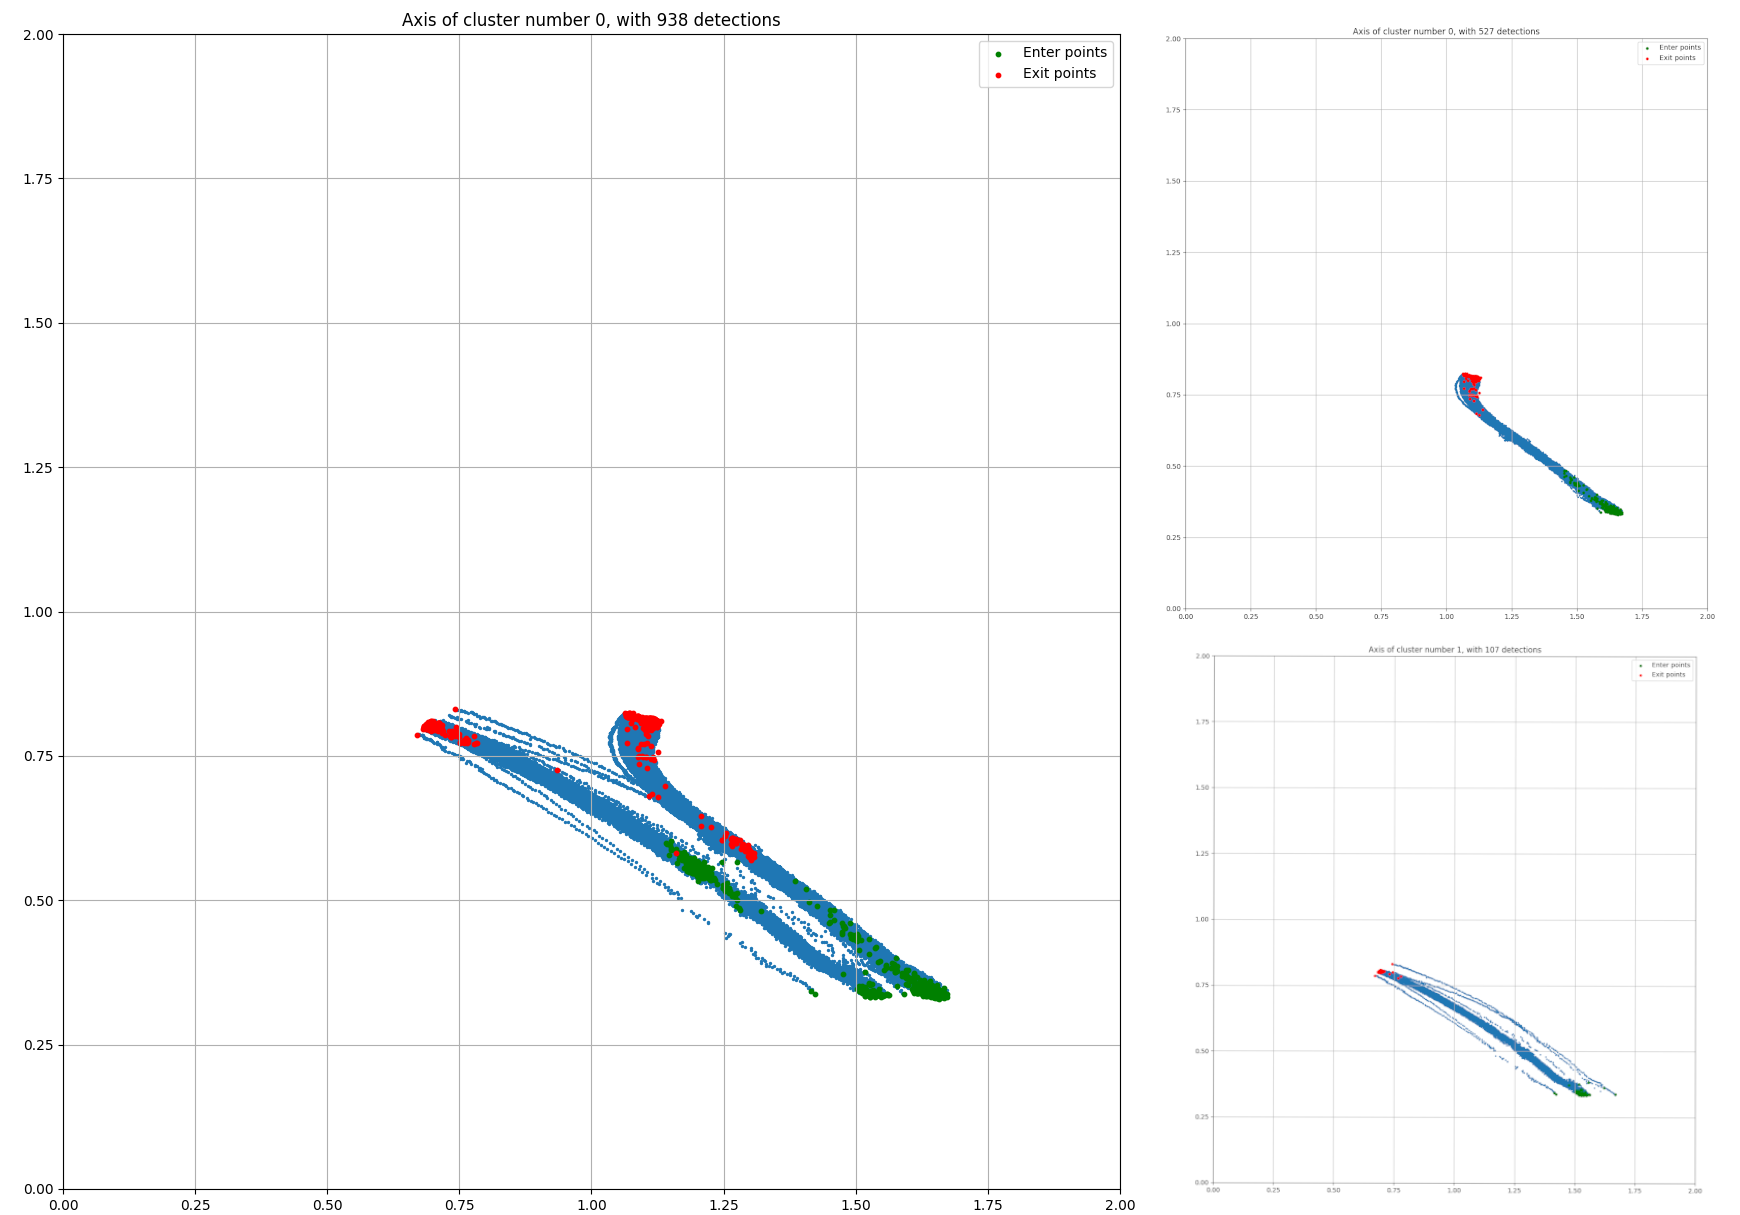
\includegraphics[width=0.65\columnwidth]{bad_clustering/example_dbscan_vs_optics_merged_cluster.png}

    \caption{KMeans, BIRCH, DBSCAN vs OPTICS}
    \label{fig: Bad clusters}
\end{figure}

\paragraph{A BIRCH (Balanced Iterative Reducing and Clustering using Hierarchies)}  egy gyors és hatékony hierarchikus klaszterezési algoritmus, amelyet nagy mennyiségű adat gyors csoportosítására fejlesztettek ki. Az algoritmus célja, hogy az adatokat összesítse a memóriában, és a klaszterek készítése során ne kelljen minden adatpontot az egész adathalmazon végigvinni.
Az algoritmus a következő lépésekből áll:
\begin{enumerate}
    \item Adatok aggregálása: Az adatok aggregálása során az algoritmus egymás mellé helyezi az adatokat az összetartozó klaszterekben. Az aggregálási folyamat során az algoritmus az adatokat kisebb csoportokba osztja, és azokat összevonja egy aggregált reprezentációba.
    \item Hierarchikus csoportosítás: Az algoritmus létrehozza az aggregált adathalmaz hierarchikus reprezentációját. Az adatokat egy fa szerkezetben helyezi el, ahol a gyökér a teljes adathalmaz, a levél pedig az egyes adatpontokat tartalmazza.
    \item Clustering: Az algoritmus elvégzi az adatok klaszterezését a hierarchikus fa struktúra alapján. A klaszterek létrehozása iteratív folyamat, amelyben az algoritmus egymás után dolgozza fel a fa szintjeit. Az algoritmus minden szinten klaszterezést végez, és az előző szinten megtalált klasztereket használja a következő szinten végzett csoportosításhoz.
\end{enumerate}
A BIRCH algoritmus előnye, hogy hatékonyan kezeli a nagy mennyiségű adatokat, és minimális memóriahasználatot igényel. Az algoritmus gyorsan fut, és lehetővé teszi a csoportok hierarchikus struktúrájának vizsgálatát. Azonban az algoritmus nem alkalmas olyan adatokra, amelyeket nehéz aggregálni, és az adatok aggregálása során elveszhetnek a finom részletek.
A futtatott tesztek alapján elmondható, hogy a BIRCH algoritmus sokszor egybevon klaszter bemeneteket vagy kimeneteket, ami miatt több más irányból jövő, vagy több más irányba kilépő objektumokat sorol azonos klaszterekbe.
\begin{math}threshold\end{math} paraméterrel lehet a klaszterek méretét szabályozni, amivel javítható az egybevont klaszterek száma, a kutatás során futtatott tesztek alapján, még így is az OPTICS adta a legtisztább klasztereket. 

\paragraph{DBSCAN (Density-Based Spatial Clustering of Applications with Noise)} egy hatékony klaszterezési algoritmus, amely a sűrűség alapján klaszterez. Az algoritmus célja, hogy megtalálja a sűrűségi alapú klasztereket az adathalmazban, és az adatpontokat azonosítsa, amelyek nem tartoznak egyik klaszterhez sem, az úgynevezett zajokat. Az algoritmus három fő paramétere a klaszterek sűrűségének küszöbe $eps$, az adatpontok minimum szomszédjainak száma $min\_samples$ és az adatpontok kiindulási pozíciója.
Az algoritmus lépései a következők:
\begin{enumerate}
    \item Választ véletlenszerűen egy adatpontot, amely még nem lett klaszterezve.
    \item Megtalálja az összes adatpontot, amelyekre az $eps$ sugarú kör középpontjából el lehet jutni.
    \item Ha az adatpontok száma nagyobb, mint a $min\_samples$, akkor létrehoz egy új klasztert és hozzáadja az összes adatpontot a klaszterhez. Ha az adatpontok száma kisebb, mint a $min\_samples$, megjelöli az adatpontot zajként.
    \item Folyamat megismétlése az összes nem klaszterezett adatponttal.
\end{enumerate}

\paragraph{Az OPTICS (Ordering Points To Identify the Clustering Structure)} egy másik klaszterező algoritmus, amely a sűrűség alapú klaszterezést használja. Az algoritmus a DBSCAN-hoz hasonlóan az adatpontok közötti sűrűségi kapcsolatokat használja a klaszterek meghatározásához, de az OPTICS további információt szolgáltat az adathalmaz klaszterezett struktúrájáról. Az algoritmus az adatpontok távolságát és azok sűrűségét is figyelembe veszi a klaszterek meghatározásához.
Az OPTICS algoritmus lépései a következők:
\begin{enumerate}
    \item Válasszunk ki egy véletlenszerű adatpontot, amely még nem került klaszterezésre.
    \item Megkeresi az összes szomszédos adatpontot, és kiszámítja a távolságot az adott adatponttól.
    \item A szomszédos adatpontokat távolság és sűrűség szerint rednezi.
    \item Létrehoz egy "optikai" sorrendet, amelyben az adatpontokat rendezzük a távolságuk és a sűrűségük szerint. Ez lehetővé teszi, hogy az algoritmus később könnyebben megtalálja a klasztereket és a zajokat.
    \item Ha az adatpontot egy klaszterhez lehet rendelni, akkor adjuk hozzá a klaszterhez.
    \item A folyamatot megismétli az összes nem klaszterezett adatpontra.
\end{enumerate}
Az OPTICS algoritmus előnye, hogy lehetővé teszi a klaszterek és a zajok meghatározását egyaránt, és további információkat is szolgáltat az adathalmaz klaszterezett struktúrájáról, mint például a klaszterek hierarchiájáról és a klaszterek közötti távolságról. Az OPTICS azonban az adathalmazok nagy méretű és magas dimenziós esetében nagyon lassú lehet, és sok erőforrást igényelhet a klaszterezéshez.

Paraméterezésben a DBSCAN annyiban különbözik az OPTICS-tól, hogy $max\_eps$ paraméter helyett, ami egy távolság tartományt ad meg, az $eps$ paramétert használja, ami pontos távolságot ad meg.

A \ref{fig: Bad clusters}. képen, a KMeans, BIRCH, DBSCAN klasztereit állítjuk szembe az OPTICS által rendezett klaszterekkel. Látható, hogy az OPTICS, nagyon hatékonyan tudta kiszűrni a zajos trajektóriákat, és nem vont egybe kimeneti vagy bemeneti klasztereket.

\subsection{Paraméterek kiválasztása}
A megfelelő paraméterek kiválasztása a klaszterezéshez igen fonzosnak bizonyult. Ezt a gyűjtött adathalmazokon kézzel kellett finomhangolnunk.
A halmazok minimum számosságát a \begin{math}min\_samples\end{math} paraméterrel lehet szabályozni, a pontok egymástól való távolságának
felső határát \begin{math}max\_eps\end{math}-el lehet megadni. Az távolság kiszámítására használt metódust \begin{math}metric\end{math}-el
lehet megadni. A \begin{math}xi\end{math} paraméterrel az elérési plot minimum meredekségét lehet megadni, ami a klaszterek határát szabja meg.
Az adathalmazra alkalmazható megfelelő paramétereket nem tudtuk generalizálni, kézzel kellett finomhangolnunk. A plotokon látható klaszterek
megtalálásához \begin{math}min\_samples=50\end{math}, \begin{math}max\_eps=0.1\end{math}, \begin{math}metric='minkowski'\end{math} és \begin{math}xi=0.15\end{math}
paramétereket használtunk.
\section{Klasszifikáció}
\subsection{Multiclass}
A több osztályos klasszifikálás egy olyan feladat, amikor több mint 2 osztály van, és minden feature vektor csak egy osztályba tartozhat. Az alapvető megközelítés a többosztályos klasszifikációra az, hogy a modell tanítása során az összes lehetséges kategóriát együttesen kell figyelembe venni. Ez azt jelenti, hogy minden egyes kategóriát egy külön osztályként kell kezelni, és a modell tanulásakor figyelembe kell venni az összes osztályt. Az osztályozó modell célja, hogy az adathalmazból kiválasztott jellemzők és az osztályok közötti kapcsolatok alapján olyan döntési fát vagy osztályozó algoritmust hozzon létre, amely képes az új adatok osztályozására. A multiclass klasszifikációhoz különböző algoritmusok használhatók, például a Random Forest, Support Vector Machine (SVM), k-Nearest Neighbor (kNN), Decision Tree és Deep Neural Network (DNN). A megfelelő algoritmus kiválasztása az adathalmaz méretétől, dimenziójától, a célkitűzésektől és az adatok jellegétől függ.
A Multiclas klasszifikáció kevesebb osztály számnál jó eredeményt adhat, a mi esetünkben 10-15 osztály is lehet, ami azt jelenti, hogy nem lehet elérni nagy pontosságot. Ennyi osztály közül nehéz pontosan eltalálni, melyik osztályba tartozik egy trajektória.
\subsection{Binary}
A binary (kétosztályos) klasszifikáció egy olyan gépi tanulási probléma, amelyben az adathalmazban szereplő objektumokat vagy eseményeket két kategóriába kell osztályozni. Például megkülönböztethetjük a "spam" és "nem spam" leveleket, vagy az "egészséges" és "beteg" betegeket az orvosi diagnózisban.
Az alapvető megközelítés a binary klasszifikációra az, hogy az osztályozó modell olyan döntési határt hoz létre az adathalmazban található adatok és az osztályok között, amely megkülönbözteti az egyik kategóriába tartozó adatokat a másiktól. Ennek az eredménye egy bináris predikció, amely azt jelzi, hogy egy adott adat az egyik vagy a másik kategóriába tartozik.
\subsection{OneVsRest}
A One-vs-Rest (OvR), más néven One-vs-All (OvA) klasszifikáció egy olyan többosztályos osztályozási technika, amelynek célja, hogy különböző osztályok között megkülönböztetést végezzen. Az OvR-ben a különböző osztályok közötti különbségeket az egyik osztályhoz képest határozzák meg. Ezt az osztályt "egy" osztálynak nevezik, és a többi osztályt "a többi" osztályoknak.
Az OvR algoritmusban egy osztályozó modellt hoznak létre minden egyes osztály és a többi osztályok közötti megkülönböztetésre. Ez azt jelenti, hogy ha van például 5 osztályunk, akkor 5 különböző bináris klasszifikátorra van szükségünk, amelyek mindegyike egy adott osztályt különböztet meg a többi osztálytól.
A bináris osztályozók által létrehozott modellt használják az osztályozásra. Az osztályozó modellnek két kimenete van, "1" vagy "0". Ha a modell kimenete "1", akkor az adott minta az adott osztályhoz tartozik, ha a kimenete "0", akkor az adott minta nem tartozik az osztályhoz.
Az OvR osztályozó előnye, hogy egyszerűen használható, mivel csak bináris osztályozókat kell alkalmazni minden egyes osztályra, és használható, ha az osztályok közötti határok nincsenek jól meghatározva.
\subsection{Machine Learning modellek}
Kutatásunk során több féle machine learning modellt teszteltünk: KNN (KNearesNeighbors), GNB (GaussianNaiveBayes), MLP (MultiLayerPerceptron), 
SGD (StochasticGradientDescent), SVM/SVC (SupportVectorMachine/SupportVectorClassifier) \cite{CC01a}, DT (DecisionTree) \cite{Breiman1984ClassificationAR}.
Ezekből a GNB, MLP és SGD nem adott jó eredményeket, ami látható az alábbi táblázatban \ref{table:1}, az eredmények megismétlődtek későbbi tesztekben, ezért
ezeket a modelleket nem tárgyaljuk. A legjobb eredményeket a KNN adta minden esetben 90\% felett teljesített. A második legjobb a DecisionTree lett, ami átlagban
balanced accuracy-ban az SVM felett teljesített, és Top 1 accuracyban is csak tizedekkel maradt le a 7. feature vektor használatakor, az 1. verzióval 4\%-al
jobban teljesített. A mérések eredményei a \ref{table:2}. és \ref{table:3}. táblázatban láthatók. 

\begin{table}[]
\centering
\begin{tabular}{|lccc|}
\hline
\multicolumn{4}{|c|}{Bellevue Newport}                                                                     \\ \hline
\hline
\multicolumn{1}{|l|}{Metrics}            & \multicolumn{1}{c|}{Balanced} & \multicolumn{1}{c|}{Top 1}   & Top 2   \\ \hline
\multicolumn{1}{|l|}{KNN}                & \multicolumn{1}{c|}{90.57\%}  & \multicolumn{1}{c|}{95.50\%} & 99.12\% \\ \hline
\multicolumn{1}{|l|}{GNB}                & \multicolumn{1}{c|}{63.92\%}  & \multicolumn{1}{c|}{73.25\%} & 90.10\% \\ \hline
\multicolumn{1}{|l|}{MLP}                & \multicolumn{1}{c|}{58.49\%}  & \multicolumn{1}{c|}{81.93\%} & 89.43\% \\ \hline
\multicolumn{1}{|l|}{SGD Modified Huber} & \multicolumn{1}{c|}{45.43\%}  & \multicolumn{1}{c|}{66.39\%} & 83.54\% \\ \hline
\multicolumn{1}{|l|}{SGD Log Loss}       & \multicolumn{1}{c|}{40.41\%}  & \multicolumn{1}{c|}{60.70\%} & 79.69\% \\ \hline
\multicolumn{1}{|l|}{SVM}                & \multicolumn{1}{c|}{77.87\%}  & \multicolumn{1}{c|}{89.29\%} & 96.61\% \\ \hline
\multicolumn{1}{|l|}{DT}                 & \multicolumn{1}{c|}{90.95\%}  & \multicolumn{1}{c|}{93.64\%} & 95.06\% \\ \hline
\end{tabular}
\caption{Bellevue Newport Feature Vektor V1}
\label{table:1}
\end{table}

\begin{table}[]
\centering
\begin{tabular}{|lccc|}
\hline
\multicolumn{4}{|c|}{\begin{tabular}[c]{@{}c@{}}Average Accuracy Feature Vector v1\end{tabular}}    \\ \hline
\hline
\multicolumn{1}{|l|}{Metrics} & \multicolumn{1}{c|}{Balanced} & \multicolumn{1}{c|}{Top 1}   & Top 2   \\ \hline
\multicolumn{1}{|l|}{KNN}     & \multicolumn{1}{c|}{94.16\%}  & \multicolumn{1}{c|}{96.71\%} & 99.46\% \\ \hline
\multicolumn{1}{|l|}{SVM}     & \multicolumn{1}{c|}{81.65\%}  & \multicolumn{1}{c|}{90.82\%} & 98.05\% \\ \hline
\multicolumn{1}{|l|}{DT}      & \multicolumn{1}{c|}{93.11\%}  & \multicolumn{1}{c|}{94.88\%} & 96.03\% \\ \hline
\end{tabular}
\caption{Testset Feature Vektor V1}
\label{table:2}
\end{table}

\begin{table}[]
\centering
\begin{tabular}{|lccc|}
\hline
\multicolumn{4}{|c|}{\begin{tabular}[c]{@{}c@{}}Average Accuracy Feature Vector v7\end{tabular}}    \\ \hline
\hline
\multicolumn{1}{|l|}{Metrics} & \multicolumn{1}{c|}{Balanced} & \multicolumn{1}{c|}{Top 1}   & Top 2   \\ \hline
\multicolumn{1}{|l|}{KNN}     & \multicolumn{1}{c|}{92.08\%}  & \multicolumn{1}{c|}{95.61\%} & 98.66\% \\ \hline
\multicolumn{1}{|l|}{SVM}     & \multicolumn{1}{c|}{88.72\%}  & \multicolumn{1}{c|}{93.86\%} & 98.92\% \\ \hline
\multicolumn{1}{|l|}{DT}      & \multicolumn{1}{c|}{89.46\%}  & \multicolumn{1}{c|}{93.30\%} & 94.55\% \\ \hline
\end{tabular}
\caption{Testset Feature Vektor V7 Stride 15}
\label{table:3}
\end{table}

\begin{table}[]
\centering
\begin{tabular}{|lccc|}
\hline
\multicolumn{4}{|c|}{\begin{tabular}[c]{@{}c@{}}Average Accuracy\\ Feature Vector v7 stride 30\end{tabular}} \\ \hline
\hline
\multicolumn{1}{|l|}{Metrics}   & \multicolumn{1}{c|}{Balanced}   & \multicolumn{1}{c|}{Top 1}    & Top 2    \\ \hline
\multicolumn{1}{|l|}{KNN}       & \multicolumn{1}{c|}{92.68\%}    & \multicolumn{1}{c|}{95.96\%}  & 98.79\%  \\ \hline
\multicolumn{1}{|l|}{SVM}       & \multicolumn{1}{c|}{88.67\%}    & \multicolumn{1}{c|}{93.49\%}  & 98.91\%  \\ \hline
\multicolumn{1}{|l|}{DT}        & \multicolumn{1}{c|}{89.87\%}    & \multicolumn{1}{c|}{93.17\%}  & 94.53\%  \\ \hline
\end{tabular}
\caption{Testset Feature Vektor V7 Stride 30}
\label{table:4}
\end{table}

\begin{table}[]
\centering
\begin{tabular}{|lccc|}
\hline
\multicolumn{4}{|c|}{\begin{tabular}[c]{@{}c@{}}Cross-Validation Average Accuracy\\ Feature Vector v1\end{tabular}} \\ \hline
\hline
\multicolumn{1}{|l|}{Metrics}     & \multicolumn{1}{c|}{Balanced}    & \multicolumn{1}{c|}{Top 1}      & Top 2      \\ \hline
\multicolumn{1}{|l|}{KNN}         & \multicolumn{1}{c|}{92.60\%}     & \multicolumn{1}{c|}{96.06\%}    & 99.38\%    \\ \hline
\multicolumn{1}{|l|}{SVM}         & \multicolumn{1}{c|}{81.21\%}     & \multicolumn{1}{c|}{89.76\%}    & 97.79\%    \\ \hline
\multicolumn{1}{|l|}{DT}          & \multicolumn{1}{c|}{92.43\%}     & \multicolumn{1}{c|}{94.55\%}    & 95.97\%    \\ \hline
\end{tabular}
\caption{Cross-Validation Feature Vektor V1}
\label{table:5}
\end{table}

\begin{table}[]
\centering
\begin{tabular}{|lccc|}
\hline
\multicolumn{4}{|c|}{\begin{tabular}[c]{@{}c@{}}Cross-Validation Average Accuracy\\ Feature Vector v7\end{tabular}} \\ \hline
\hline
\multicolumn{1}{|l|}{Metrics}     & \multicolumn{1}{c|}{Balanced}    & \multicolumn{1}{c|}{Top 1}      & Top 2      \\ \hline
\multicolumn{1}{|l|}{KNN}         & \multicolumn{1}{c|}{90.74\%}     & \multicolumn{1}{c|}{95.49\%}    & 98.39\%    \\ \hline
\multicolumn{1}{|l|}{SVM}         & \multicolumn{1}{c|}{87.36\%}     & \multicolumn{1}{c|}{94.03\%}    & 98.85\%    \\ \hline
\multicolumn{1}{|l|}{DT}          & \multicolumn{1}{c|}{89.12\%}     & \multicolumn{1}{c|}{93.56\%}    & 94.95\%    \\ \hline
\end{tabular}
\caption{Cross-Validation Feature Vektor V7 Stride 15}
\label{table:6}
\end{table}

\begin{table}[]
\centering
\begin{tabular}{|lccc|}
\hline
\multicolumn{4}{|c|}{\begin{tabular}[c]{@{}c@{}}Cross-Validation Average Accuracy\\ Feature Vector v7 stride 30\end{tabular}} \\ \hline
\hline
\multicolumn{1}{|l|}{Metrics}       & \multicolumn{1}{c|}{Balanced}       & \multicolumn{1}{c|}{Top 1}         & Top 2        \\ \hline
\multicolumn{1}{|l|}{KNN}           & \multicolumn{1}{c|}{91.15\%}        & \multicolumn{1}{c|}{95.64\%}       & 98.54\%      \\ \hline
\multicolumn{1}{|l|}{SVM}           & \multicolumn{1}{c|}{87.28\%}        & \multicolumn{1}{c|}{93.69\%}       & 98.60\%      \\ \hline
\multicolumn{1}{|l|}{DT}            & \multicolumn{1}{c|}{89.55\%}        & \multicolumn{1}{c|}{93.73\%}       & 95.15\%      \\ \hline
\end{tabular}
\caption{Cross-Validation Fetature Vektro V7 Stride 30}
\label{table:7}
\end{table}

\paragraph{A K-Nearest Neighbors (KNN)} egy egyszerű és hatékony osztályozó algoritmus, amely az adatok közötti távolság alapján osztályozza a bemeneti adatokat. Az algoritmus lényege, hogy egy adott bemeneti adathoz hasonló adatokat keres a tanuló adathalmazból, majd azok osztálycímkéit megnézve meghatározza az adat osztályát. 
Az algoritmus először szükséges, hogy az adatokat előkészítse. Ez magában foglalhatja az adatok normalizálását, standardizálását, az outlier-ek kezelését, valamint a kategorikus adatok konvertálását numerikus formába.
Az algoritmus működése a következő lépésekből áll:
\begin{enumerate}
    \item Távolságok számítása: Az algoritmus először számítja ki az összes tanuló adatpont és a bemeneti adatpont közötti távolságot. A leggyakrabban használt távolságmértékek az euklideszi és manhattani távolságok.
    \item K legközelebbi szomszéd kiválasztása: Az algoritmus a távolságok alapján kiválasztja a K legközelebbi szomszédot a bemeneti adatpontnak. A K értéke általában egy páros szám, hogy elkerüljük a döntések holtversenyét.
    \item Döntés meghozása: Az algoritmus a K legközelebbi szomszéd osztálycímkéinek többségi szavazatával dönti el, hogy melyik osztályba sorolja a bemeneti adatpontot.
\end{enumerate}
Az előnye, hogy a KNN algoritmus könnyen értelmezhető és egyszerűen használható. Az algoritmus jól működik a kisebb méretű adathalmazokon, különösen akkor, ha az adatok egyszerű struktúrával rendelkeznek. A KNN továbbá jól alkalmazható olyan feladatokra, ahol a határok nem lineárisak, és ahol a szokásos statisztikai módszerek nem elegendőek. Az algoritmusnak azonban vannak korlátai, például az, hogy az algoritmus futási ideje növekszik az adathalmaz méretével, valamint hogy az eredmények érzékenyek lehetnek az adatpontok elhelyezkedésére.

\paragraph{Az SVM (Support Vector Machine)} egy erőteljes, nemlineáris osztályozó algoritmus, amelynek célja egy határvonal (vagy hipersík) megtalálása az adatok között. Az algoritmus a bemeneti adatokat olyan módon osztályozza, hogy a döntési határvonal az osztályok közötti legnagyobb távolságot biztosítsa. Ez a távolság a két legközelebbi adatpont közötti távolság, és margin-nek nevezik.
Az SVM algoritmus működése a következő lépésekből áll:
\begin{enumerate}
    \item Adatok előkészítése: Az adatokat előkészítjük, eltávolítjuk a hiányzó adatokat, valamint normalizáljuk vagy standardizáljuk az adatokat a hatékonyabb tanulási folyamat érdekében.
    \item Határvonal (hipersík) keresése: Az SVM algoritmus az adatokat olyan módon osztályozza, hogy a határvonal a két osztály közötti legnagyobb távolságot biztosítsa. Az algoritmus megtalálja az optimális hipersíkot, amely a legnagyobb margin-t biztosítja, amely egyenlő a két legközelebbi adatpont távolságával.
    \item Osztályozás: Az algoritmus az új adatokat a hipersíkon való pozíciójuk alapján osztályozza. Az algoritmus eldönti, hogy az új adat melyik oldalon található a határvonalon.
\end{enumerate}
Az SVM előnye, hogy jól működik a magas dimenziós adatokon és olyan feladatokon, ahol az osztályok közötti határok nem lineárisak. Az SVM továbbá rendkívül hatékony az outlier-ek kezelésében, mivel csak azok a pontok határozzák meg a határvonalat, amelyek a legközelebb vannak hozzá. Az SVM azonban egy nehézkes algoritmus, amelynek tanítása hosszabb ideig tart, ha nagy adathalmazokat kell kezelni. Az algoritmus hiperparamétereinek finomhangolása továbbá kihívást jelenthet, különösen ha nem rendelkezünk megfelelő előzetes tudással az adathalmazról.
\paragraph{SVM Paraméterek} Több féle "kernel function" - szűrő - közül választhatunk, ami lehet lineáris, polinomiális, exponenciális stb. Mi az RBF (Radial Basis Function) exponenciális szűrőt használtuk, aminek két fő paramétere van: $C$ és $\gamma$. $C$ az SVM egy általános paramétere, ami másik szűrők használatakor is jelen van. Ez a paraméter határozza meg mennyire legyen elsimítva az osztályok közötti határ. Alacsony $C$ sima határvonalhoz vezet, amíg a magas $C$ azt okozza, hogy minden tanító adatot pontosan osztályozni tudjon. A $\gamma$ prarméter, azt határozza meg, hogy egy tanító adatnak mekkora befolyása van. Magas $\gamma$ esetén az egymáshoz közelebbi adatok magas befolyással bírnak egymásra. Méréseink során azt tapasztaltuk, hogy az SVM tényleg gyors és hatékony, még nagy tanító halmaz mellett is.

\paragraph{A Decision Tree (döntési fa)} egy olyan algoritmus, amely a bemeneti adatok alapján egy hierarchikus fastruktúrát hoz létre. Az ilyen fastruktúra minden csomópontjában egy adatfajta tulajdonsága áll, és a levélcsomópontokban pedig a végleges osztálycímkék találhatók. A döntési fában minden ág egy adott tulajdonság értékét reprezentálja, és a fa felépítése során az algoritmus igyekszik minél jobban felosztani a bemeneti adatokat az osztályok között.
A Decision Tree osztályozó algoritmus létrehozása során a következő lépések szükségesek:
\begin{enumerate}
    \item Adatok előkészítése: Az adatokat elő kell készíteni az osztályozó algoritmus számára, amely magában foglalhatja az adatok előfeldolgozását, a hiányzó értékek kezelését és a kategórikus változók átalakítását számszerű adatokká.
    \item Fa építése: A faépítés során az algoritmus megpróbálja kiválasztani a legmegfelelőbb tulajdonságot a bemeneti adatok osztályozásához, majd a tulajdonság értékeitől függően felosztja az adatokat az algoritmus által meghatározott csoportokba. Az algoritmus folytatja ezt a folyamatot minden ágba, amíg el nem éri a megállási feltételt.
    \item Fa értékelése: Az értékelés során az algoritmus osztálycímkéket rendel a bemeneti adatokhoz a fa segítségével.
\end{enumerate}
A döntési fa osztályozó algoritmus előnye, hogy a modell könnyen értelmezhető és átlátható, így könnyen megérthető, hogy a modell hogyan dönt a különböző osztálycímkékkel kapcsolatban. Az algoritmus továbbá jól alkalmazható kategórikus és numerikus változók kezelésére, valamint skálázható és gyorsan futtatható nagyobb adathalmazokon is.
Egy döntési fát könnyű vizualizálni és kirajzolni, hisz egyszerű "if-else" logikai elágazásokból épül fel (lásd \ref{DTVis}). Nagy és komplex fák alakulhatnak ki, amik túltanulást eredményezhetnek, és már kis eltérések a tanító halmazban nagy eltéréseket eredményezhetnek a fa logikájában.

\begin{figure}
    \centering
    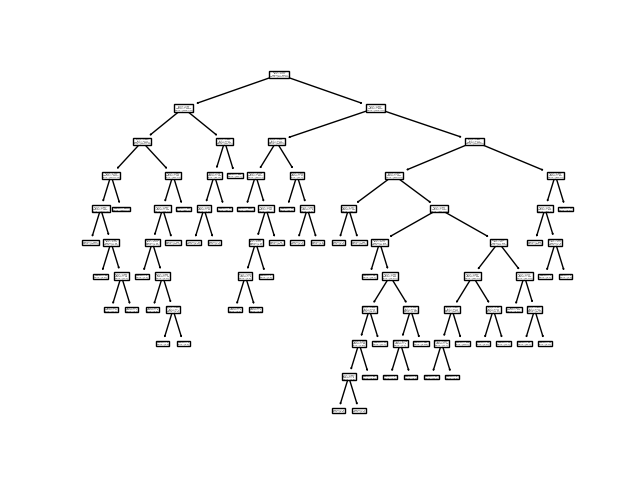
\includegraphics[width=1.2\columnwidth]{visualization/bellevue_eastgate_DT_2.png}
    \caption{DecisionTree Visualization}
    \label{DTVis}
\end{figure}

\subsection{Feature vektorok}
Ahogyan klaszterezésnél is, fontos meghatározni egy olyan feature vektort, ami a legjobban jellemzi a trajektóriát. Ebben a papírban
két fajta vektor verziót fogunk tárgyalni, amik a tesztek során a legjobban teljesítettek. Az egyik a legelső verzió amit kipróbáltunk,
a másik a hetedik verzió, ami jobban teljesített, mint az összes többi 2-6 verzió. 
\paragraph{Az első verzió} Felépítése a következő \begin{math}[x_0, y_0, v_{x_0}, v_{y_0}, x_m, y_m, x_l, y_l, v_{x_l}, v_{y_l}]\end{math}, ahol \begin{math}m\end{math}
index jelöli az időben középen elhelyezkedő detektálást, az \begin{math}l\end{math} index pedig az utolsó, legfrissebb detektálást jelőli.
Ez a vektor jól reprezentálja a valós idejű futás közben keletkező trajektóriákat, mert egyszerre több száz detektálást objektumonként
nem lehet eltárolni a memórában, hanem egy meghatározott méretű buffert kell alkalmazni, aminek mi 15 vagy 30 detektálást adtunk.
Az adathalmazban eltárolt trajektóriák ennél a buffernél több detektálást tartalmaznak, ezért az első verziónál a trajektóriát \begin{math}k\end{math} 
részre osztottuk, így egy trajektória szelet mérete \begin{math}s_n = n_d/k\end{math}, ahol \begin{math}n_d\end{math} a detektálások számossága
a trajektóriában. Ezekből a szeletekből képeztük az egyes feature vektorokat.
\paragraph{A hetedik verzió} Felépítése \begin{math}[x_0 \cdot w_1, y_0 \cdot w_2, v_{x_0} \cdot w_3, v_{y_0} \cdot w_4, x_l \cdot w_5, y_l \cdot w_6, v_{x_l} \cdot w_7, v_{y_l} \cdot w_8]\end{math}.
Ennél a verziónál használtunk súlyokat, ahol \begin{math}w_1=1\end{math}, \begin{math}w_2=1\end{math}, \begin{math}w_3=100\end{math}, \begin{math}w_4=100\end{math},
\begin{math}w_5=2\end{math}, \begin{math}w_6=2\end{math}, \begin{math}w_7=200\end{math}, \begin{math}w_8=200\end{math}. Mivel a sebességek két 
nagyságrenddel kisebbek mint a koordináták, ezért felszoroztuk őket 100-as súlyokkal. Hogy a 15-30 detektálás nagyságú bufferekben nagyobb hangsúlyt kapjanak a legfrissebb
koordináták és sebességek, így azok 2-es és 200-as szorzót kaptak. A mérések ereményéből azt lehet levonni, hogy a 30-as bufferméret használata nem kifizetődő, hiszen nem növekedett a pontosság, és kétszer akkora memória igénye van.
\paragraph{Teszt eredmények} Azt mutatják, hogy az utóbbi verzió növelte az SVM pontosságát, viszont rontott a KNN és DT pontosságán (lásd \ref{table:3}). Még nagyobb adathalmazok esetén, ahol pár ezer trajektória helyett több tíz vagy akár százezer van, érdemes megfontolni, hogy a 7. verzióval tanítunk be SVM modellt, mivel a KNN futási ideje ekkora adatmennyiség esetén sokkal lassabb lesz.

\subsubsection{Adatdúsítás}
Hogy minél pontosabban reprezentáljuk a valód idejű futást és növeljük a tanító adathalmazt, egy trajektóriából több feature vektort állítunk elő.
Ezeknek a számosságát, a feature vektorokat generáló algoritmusban szabtuk meg. Ezzel azt is szabályoztuk, hogy mekkora időszeletből prediktáljon
a modellünk. Mint ahogy fent is említettük, valós időben 15, max 30 detektálást érdemes tárolni a bufferben. A mérési eredmények azt mutatják, hogy
15 és a 30 nagyságú buffer közt nincs nagy különbség pontosságban. Futási idő szempontjából érdemes lehet a 15 nagyságú buffert választani,
ha van elég tanító adat, és időt akarunk spórolni tanításnál, akkor a 30 nagyságú buffert is választhatjuk, mivel így felére csökken a feature vektorok száma, ez kevesebb tanítási időt jelent, viszont futás közben lesz nagyobb a memóriaigény.
%\subsubsection{Klassz kiegyenlítés}
\subsection{Pontosság mérése}
A pontosság mérésére háromféle metrikát használtunk.
\paragraph{Accuracy Score}
Ha \begin{math}\hat{y_i}\end{math} az \begin{math}i\end{math}. minta predikciója és \begin{math}y_i\end{math} a hozzátartozó valódi érték,
akkor az eltalált predikciók és összes predikció hányadosa, amit így lehet leírni:\break
\begin{equation}
\texttt{accuracy}(y, \hat{y}) = \frac{1}{n_\text{samples}} \sum_{i=0}^{n_\text{samples}-1} 1(\hat{y}_i = y_i)
\end{equation}
\paragraph{Balanced Accuracy}
amit azért használtunk, hogy az adathalmaz kiegyensúlyozatlansága miatt ne kapjunk fals pontosságot. Ha minden osztályra egyenlően jól teljesít a klasszifikációs modellünk, akkor a sima \emph{Accuracy}-t kapjuk vissza.
Ha a teszt adathalmaz kiegyensúlyozatlansága miatt az egyik osztálynak jobb a pontossága, mint egy másiknak, akkor ezt az értéket elosztja a számával. Ha az \begin{math}y_i\end{math} a valódi értéke az \begin{math}i\end{math}. mintának, és \begin{math}w_i\end{math} a hozzátartozó súly, akkor ezt a súlyt a következőképpen korrigáljuk:
\begin{equation}
    \hat{w}_i = \frac{w_i}{\sum_j{1(y_j = y_i) w_j}}
\end{equation}
ahol \begin{math}1(x)\end{math} a karakterisztikus függvény. Adott a \begin{math}\hat{y_i}\end{math} perdikció az \begin{math}i\end{math}.
mintának, így a balanced accuracy-t így definiálhatjuk:
\begin{equation}
    \texttt{balanced-accuracy}(y, \hat{y}, w) = \frac{1}{\sum{\hat{w}_i}} \sum_i 1(\hat{y}_i = y_i) \hat{w}_i
\end{equation}
\paragraph{Top-K Accuracy}
az \emph{Accuracy Score} egy generalizált változa-ta. A különbség az, hogy a predikció akkor számít igaznak, ha beletartozik a \begin{math}k\end{math}
legmagasabb valószínűségű predikciók közé. Ha \begin{math}\hat{f}_{i,j}\end{math} a \begin{math}i\end{math}. mintának a \begin{math}j\end{math}. legmagasabb 
predikciója, és \begin{math}y_i\end{math} a hozzátartozó valódi predikció, akkor az eltalált predikciók és az összes minta hányadosát így
lehet definiálni:
\begin{equation}
    \texttt{top-k accuracy}(y, \hat{f}) = \frac{1}{n_\text{samples}} \sum_{i=0}^{n_\text{samples}-1} \sum_{j=1}^{k} 1(\hat{f}_{i,j} = y_i)
\end{equation}
ahol \begin{math}k\end{math} a megengedett találgatások száma, és \begin{math}1(x)\end{math} a karakterisztikus függvény.
\subsubsection{Adathalmaz szétválasztás}
A pontosság méréséhez el kell választanunk egy teszt adatahalmazt a tanító adathalmaztól, mivel ha azon az adathalmazon tesztelünk, amin tanítottunk,
akkor tökéletes pontosságot kapnánk eredményül. Ezt \emph{Overfitting}-nek hívják. A szétválasztást egy általunk implementált algoritmus végzi, ami véletlen szám generátort használ a
minták kiválasztásához. Az algoritmusnak meg lehet adni paraméterként a tanító adathalmaz méretét, és egy \emph{seed} értéket, ami azért fontos, hogy meg
lehessen ismételni a szétválasztást.
\subsubsection{Cross Validation}
A túltanítás elkerülése érdekében, alkalmaztunk egy elterjedt metódust a cross-validációt. A cross validáció egy olyan metódus, ahol a tanító adathalmazt
$k$ részre osztják, ebből a $k$ részből egyet kiválasztanak validációra, így keletkezik egy tanító és validáló adathalmaz. A tanító adathalmazon betanítanak
egy modellt, aminek a pontosságát megmérik a validáló adathalmazon. Ezt az algoritmust $k$-szor ismétlik meg, úgy hogy minden rész egyszer legyen validáló
adathalmaz. Ezeknek a méréseknek az átlag pontosságát szokták kiszámolni. A cross-validációból származó eredmények a \ref{table:4}. és \ref{table:5}. 
táblázatban mutatjuk be.
\subsubsection{Teszthalmazos validáció}
Hogy meggyőződjünk arról, hogy biztosan nem tanítottuk túl a modellünket, egy olyan teszt adathalmazon is le kell tesztelnünk, amit nem használtunk fel egyszer sem
cross-validáció alatt tanításra. Ezzel a méréssel bebizonyosodhatunk róla, hogy a modellünkben nincsen bias. A teszthalmazos mérés eredményeit a \ref{table:2}. és \ref{table:3}.
táblázatban mutatjuk be.
\subsubsection{Modellek tárolása}
A betanított modelleket joblib file-ként tároltuk el, amit később python-nal tudunk betölteni.

\newpage
\section{Valós idejű alkalmazás}
A modellek pontosságának tesztelésére nem csak mérőszámokat alkalmaztunk, hanem egy vizualizációs alkalmazást is fejlesztettünk. Az alkalmazásnak meg kell adni
a joblib modell fájlt és a videót, amin tanítottuk. Ezeken kívül meg lehet adni mekkora detekció buffert használjon és hogy a top mennyi predikciót rajzolja ki.
A lejátszó kirajzolja a klaszterek kimeneti pontjait, és az autók középpontjával köti össze. A legvalószínűbb predikció zölddel, a kevésbé valószínű pedig pirossal
van kirajzolva (lásd \ref{BellevueNewportRealTime} \ref{fig: BellevueNERealTime} \ref{fig: BellevueSERealTime} \ref{fig: BellevueEastgateRealTime}). 
Az alkalmazás futását a mellékletben megadott videókon lehet megtekinteni.

\begin{figure}[H]
    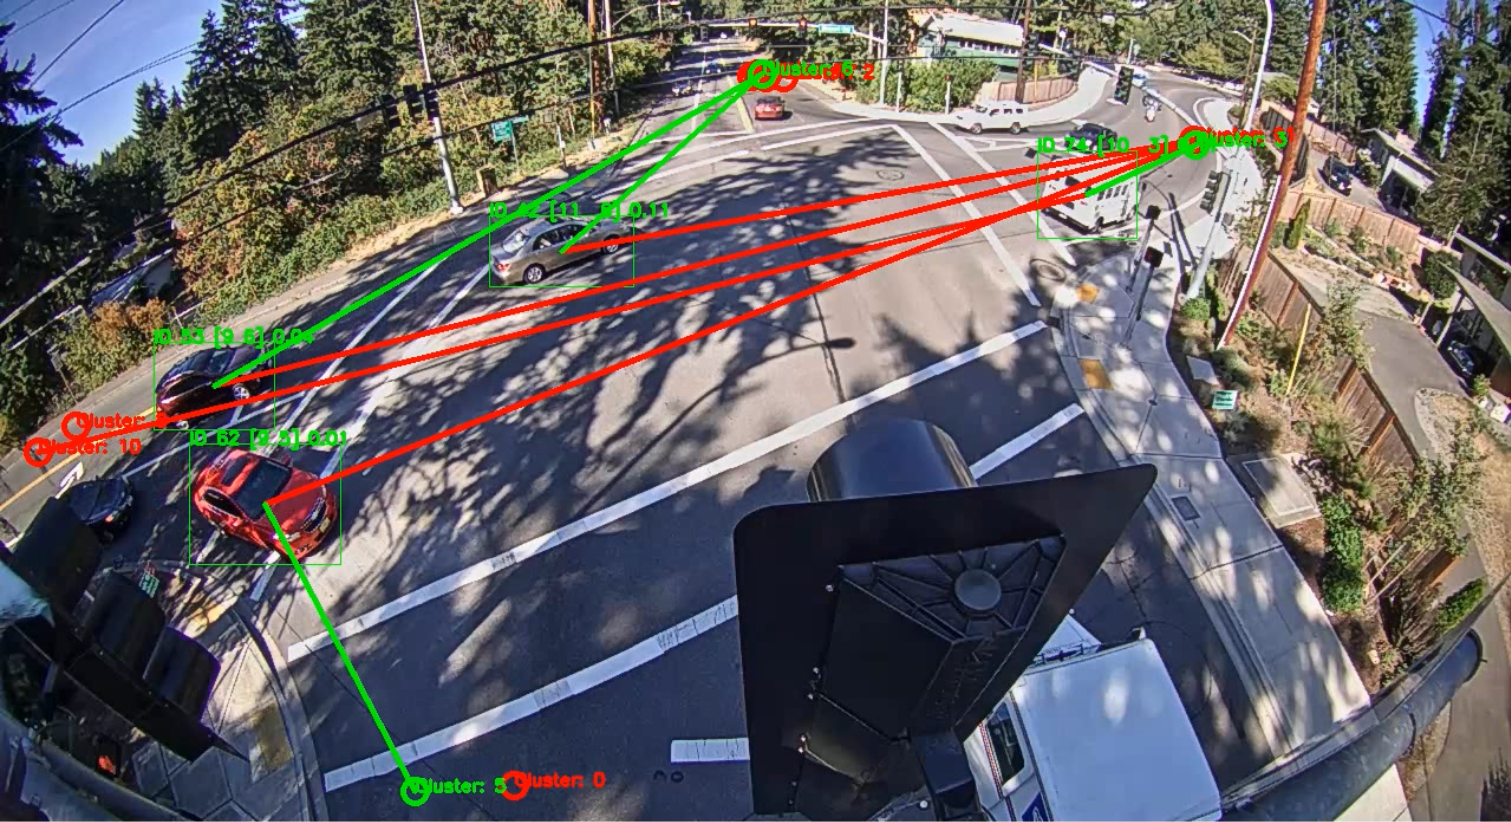
\includegraphics[width=1\columnwidth]{visualization/bellevue_newport.png}
    \caption{Bellevue Newport real time application}
    \label{BellevueNewportRealTime}
\end{figure}

\begin{figure}[H]
    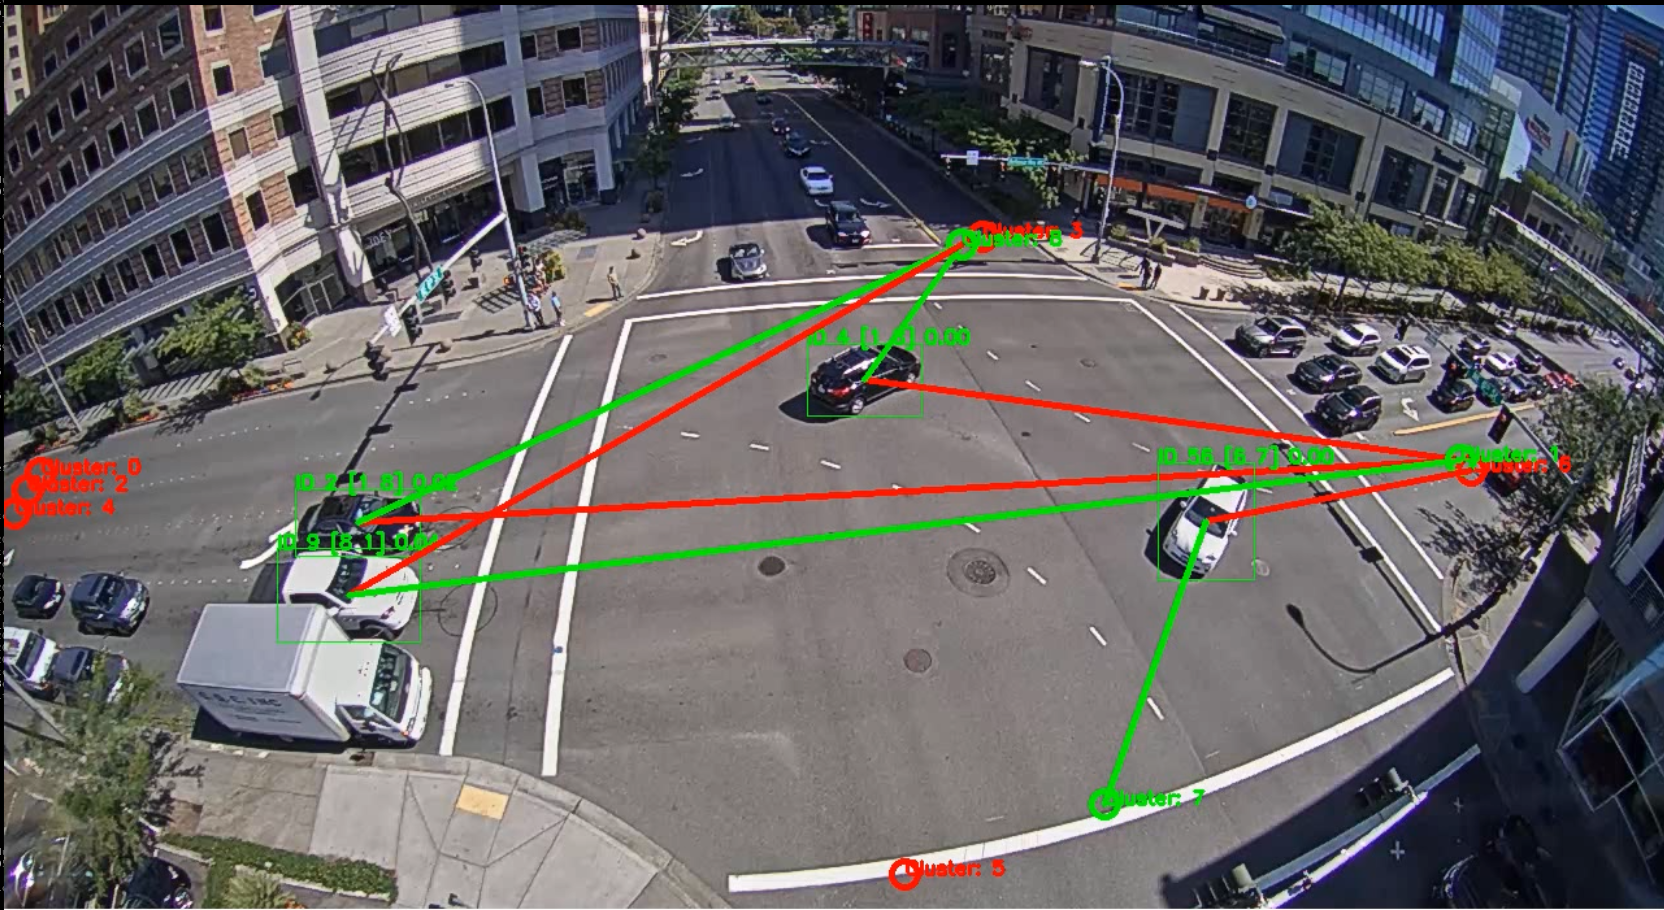
\includegraphics[width=1\columnwidth]{visualization/bellevue_ne.png}
    \caption{Bellevue NE real time application}
    \label{fig: BellevueNERealTime}
\end{figure}

\begin{figure}[H]
    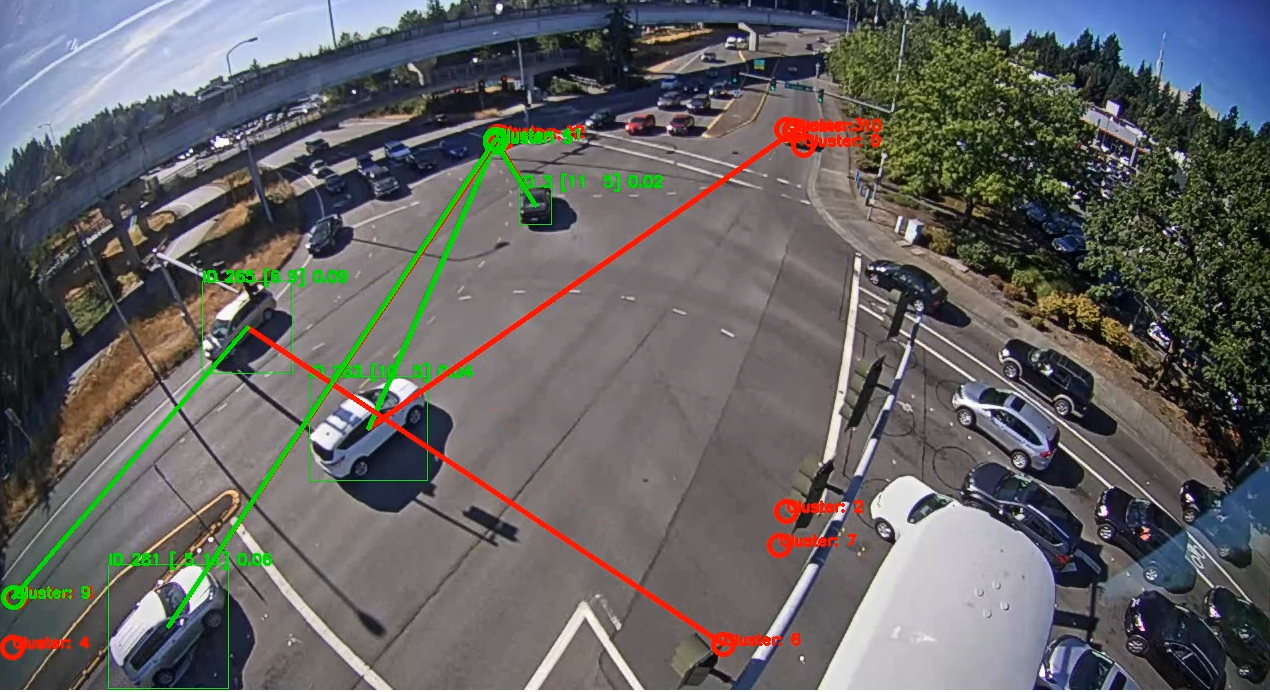
\includegraphics[width=1\columnwidth]{visualization/bellevue_eastgate.png}
    \caption{Bellevue Eastgate real time application}
    \label{fig: BellevueEastgateRealTime}
\end{figure}

\begin{figure}[H]
    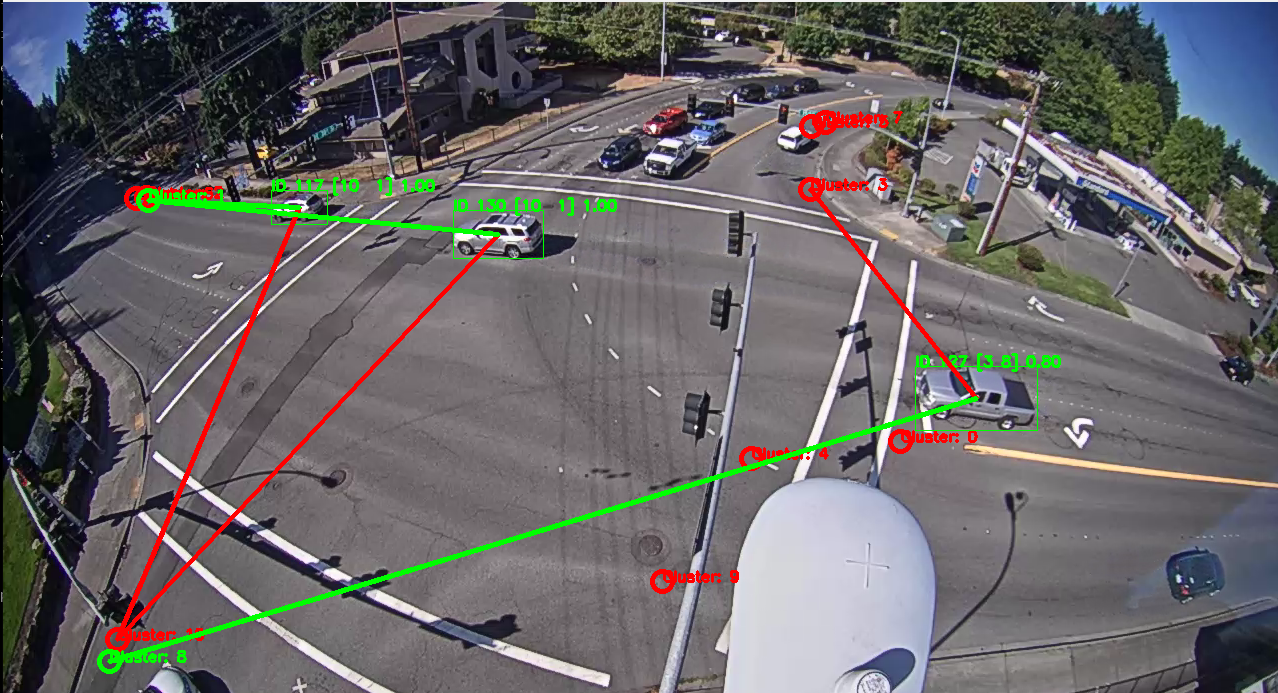
\includegraphics[width=1\columnwidth]{visualization/bellevue_se.png}
    \caption{Bellevue SE real time application}
    \label{fig: BellevueSERealTime}
\end{figure}

\section{Konklúzió}
A kiépített keretrendszer a klaszterezéssel és klasszifikációs modellek betanításával egy fontos lépés ezen terület fejlesztésében. A mérések jó alapot szolgálnak a jövőbeli kutatásoknak, milyen algoritmusokat érdemes még mélyebben megvizsgálni és melyekkel nem érdemes a továbbiakban foglalkozni. Más objektumdetektáló és objektumkövető algoritmusokat is érdemes lehet kipróbálni, amiviel az adatgyűjtési fázist és az adattisztítási fázist lehet felgyorsítani és hatékonyabbá tenni.
Az átlagos 90\% pontosság, amit elértünk a tanított modellekkel, nem tűnik túl magasnak, de figyelembe kell vennünk, hogy egy autó mozgása során sok olyan időszakasz van, amikor lehetetlen előre megmondani, melyik útvonalat fogja választani, mert pl. csak közelít a kereszteződéshez és nem választott még sávot. Ilyenkor az autó mozgása még semmilyen szinten nem utal a későbbi pályára, ezért óhatatlanul tévedések következnek be. A módszer predikciós képességét ilyenkor a "top-2 accuracy" mutatja: a tipikusan 10-15 lehetséges útvonal-csoport közül a választott 2 legvalósíznűbb már 95\% feletti eséllyel tartalmazza a ténylegesen bekövetkezőt. 
Viszont adathalmaz növelésével ezt a jövőben még növelni lehet. A feature vektorok dimenziószámának növelésével és másfajta súlyozással is növelhető ez a pontosság. A dimenzió növelése felveti a lehetőséget, hogy a jövőben mély neurális hálókat is teszteljünk az osztályozás feladatra.
A megerősító tanulás bevezetése a keretrendszerünke is egy nagy előrelépés lehet, ezt úgy lehetne megvalósítani, hogy valós idejű futás közben, a bejövő adatokon nem csak osztályozást végzünk hanem ezeket az adatokat folyamatosan mentjük, majd ha elég adat összegyűlt időközönként frissítjük a modellt, így a modell adaptálódni tud a forgalom változásához. 
%\section{Alkalmazási területek}

\newpage
\printbibliography
\end{document}